\engine{2}
\title{3d Brownian motion and sets of dimension 2.99999}
\course{Mathematics Colloquium · Washington University in St. Louis}
\author{Matthew Badger · University of Connecticut}
\date{November 19, 2026}
\copyright{M. Badger · WUSTL 2026}
\footer{section}
\autofit{1.45}
\spread{on}
% Color scheme used throughout:
%   c1 (blue)   dimension, holes, covers, Hausdorff contents
%   c3 (purple) harmonic measure, barriers
%   c2 (orange) volume
%   c4 (green)  new results
%   alert (red) the headline numbers
% Slide text has no terminal period; periods appear only between consecutive sentences.
\newcommand{\side}{\operatorname{side}}
\newcommand{\vol}{\operatorname{vol}}
\newcommand{\Haus}{\mathcal{H}}
\newcommand{\RR}{\mathbb{R}}
\newcommand{\udim}{\overline{\dim}_H}
\newcommand{\Prob}{\mathbf{Prob}}

\titleslide
Joint with \textbf{Michael Albert} (Okinawa Institute of Science and Technology) and \textbf{Alyssa Genschaw} (Milwaukee School of Engineering)
\vfill
\small{Partially supported by NSF DMS 2154047}

\slide[valign=center, align=center]{}
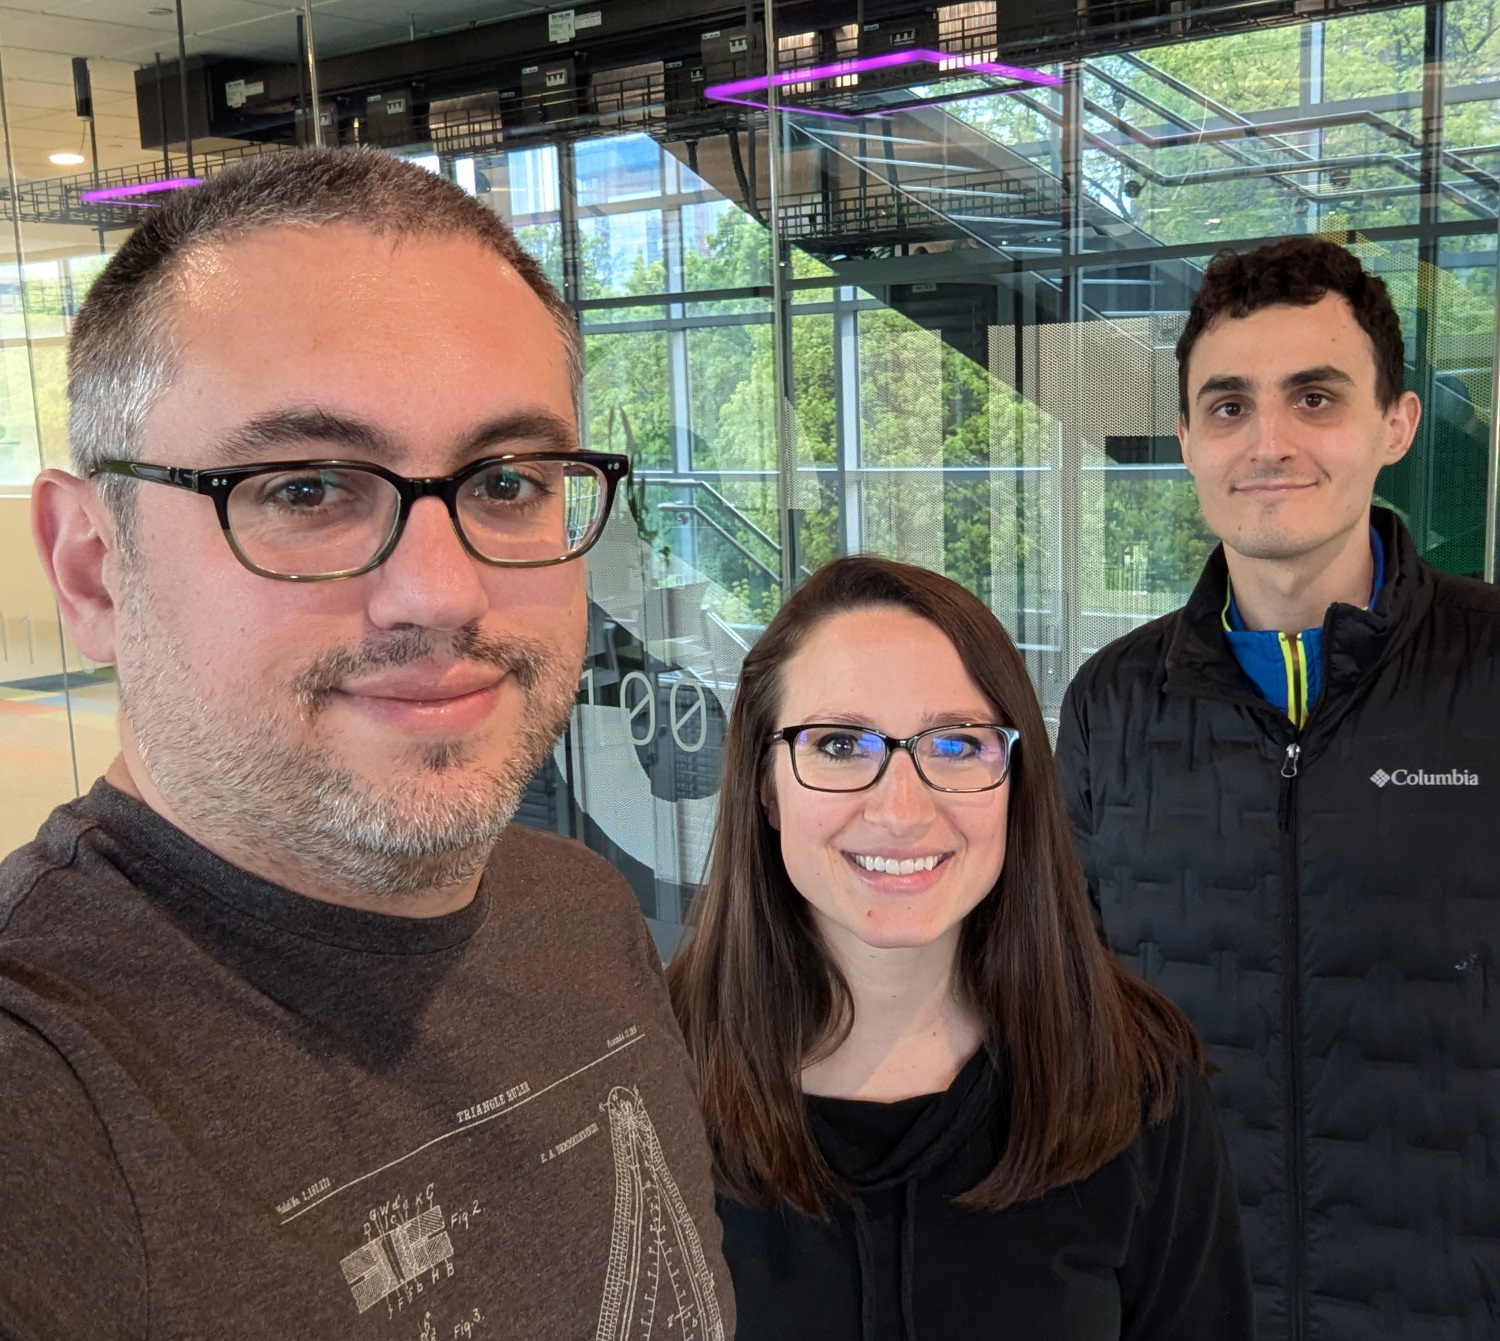
\includegraphics[height=600, alt="Michael Albert, Matthew Badger, and Alyssa Genschaw"]{albert-badger-genschaw.jpg}
The team: Michael Albert, Matthew Badger, Alyssa Genschaw at the \textcolor{c2}{Milwaukee School of Engineering}, Summer 2025

Alyssa is an Associate Professor at MSOE. Michael is now a postdoc at the \textcolor{c1}{Okinawa Institute of Science and Technology}

\slide{A question about breathing}
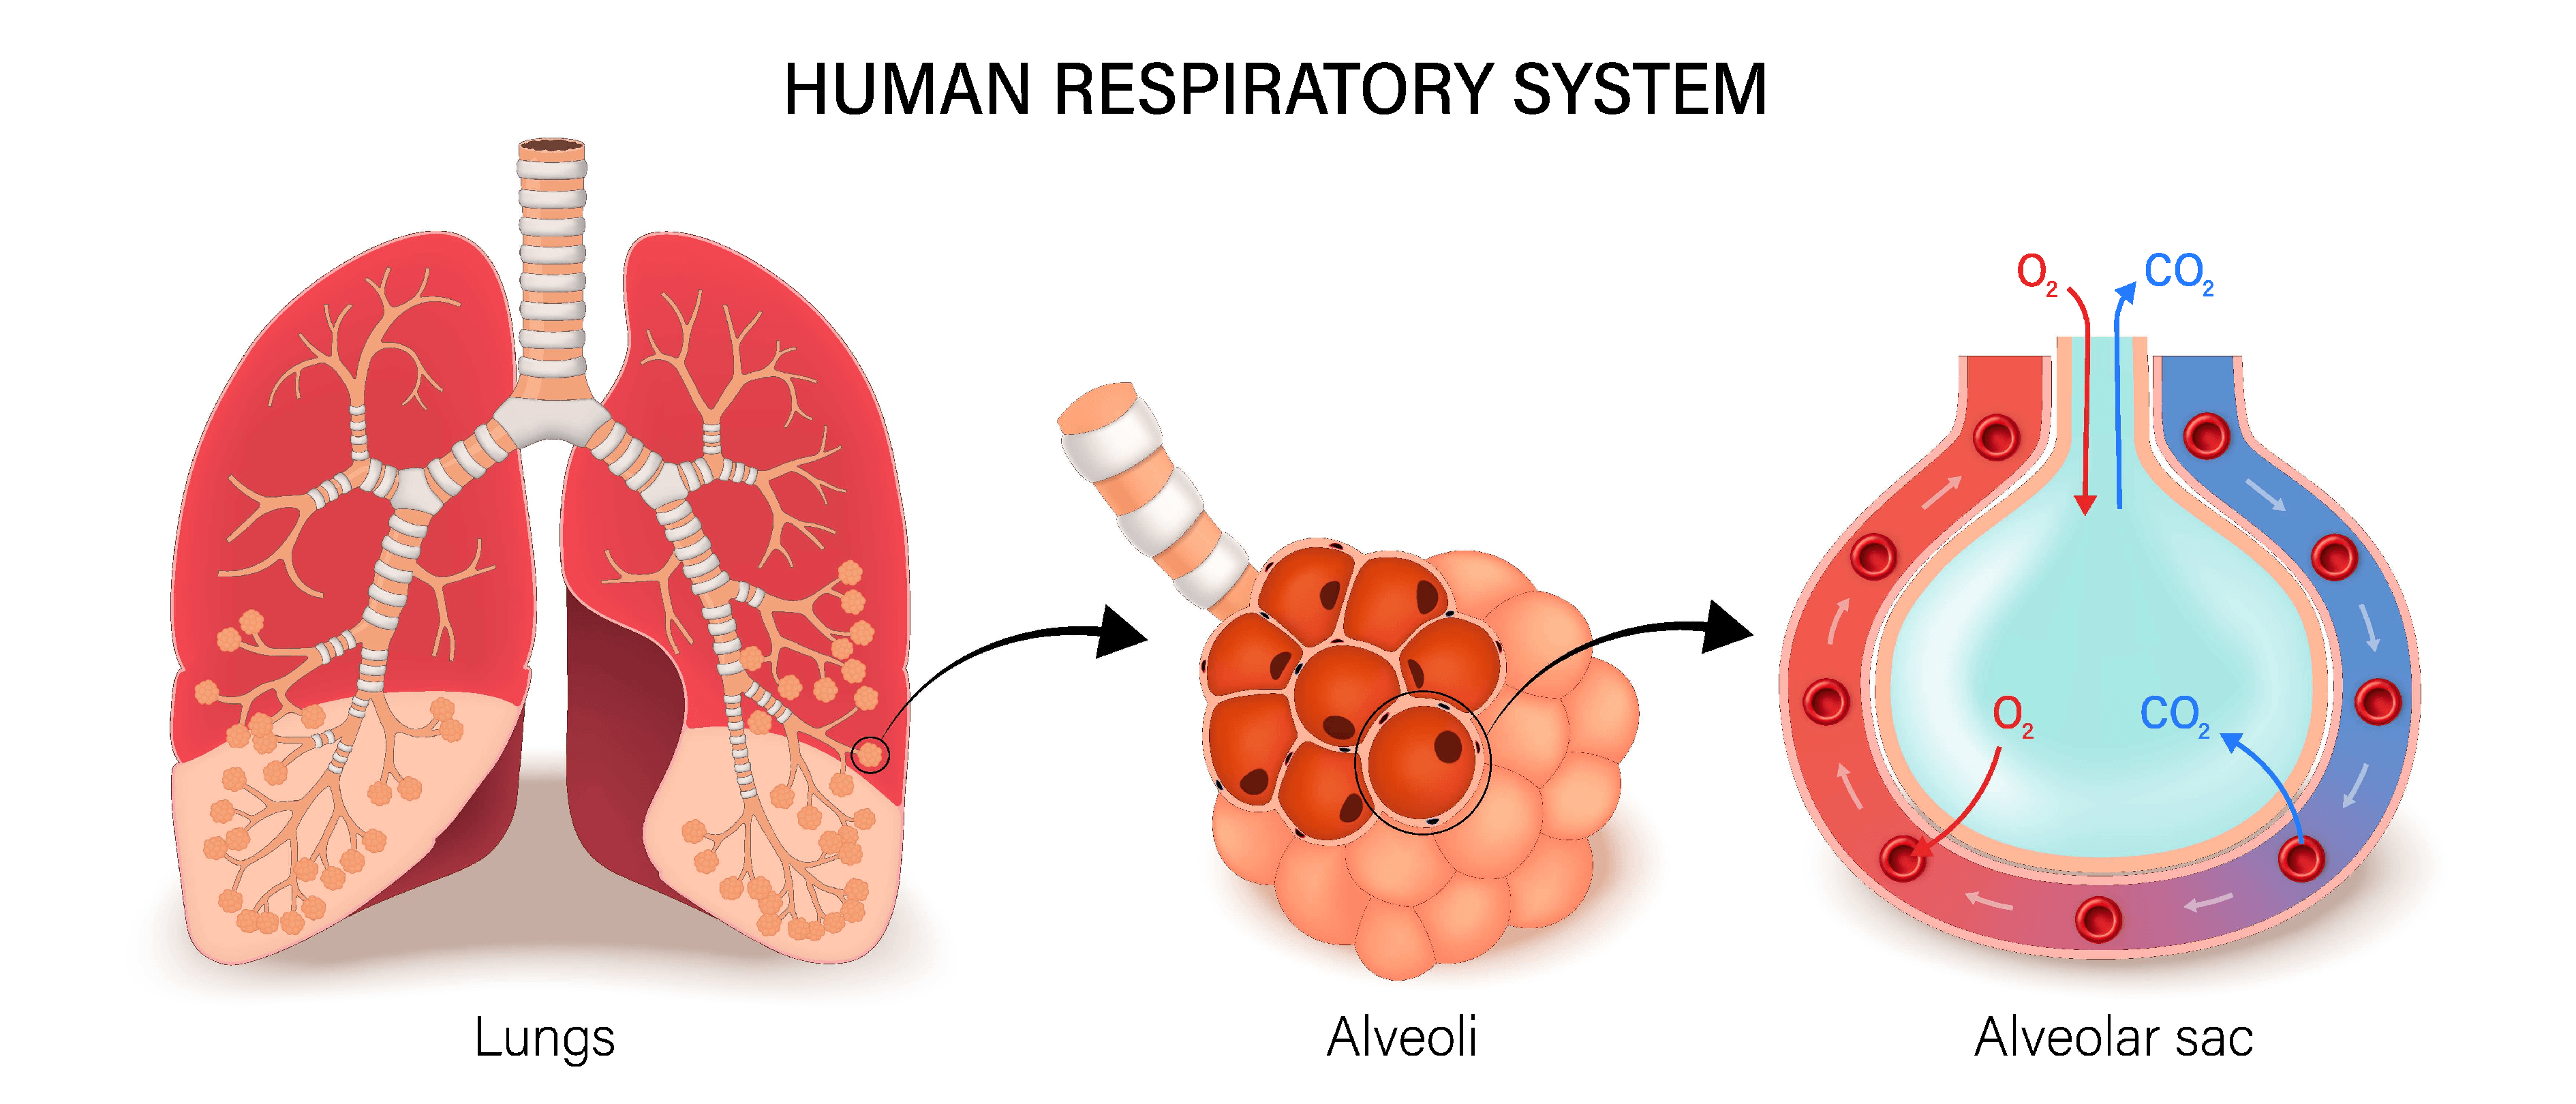
\includegraphics[height=520, alt="The human respiratory system: lungs, a cluster of alveoli, and one alveolar sac where oxygen passes into the blood"]{lungs.png}
\begin{columns}[1 1]
As you breathe, air eventually reaches the \textcolor{c3}{alveoli} in your lungs
\medskip
\textbf{Is a particle of air equally likely to reach every part of your lungs?}
\columnbreak
\begin{itemize}
\item about $480{,}000{,}000$ alveoli in human lungs
\item one alveolus: diameter $200$–$500\,\mu m$
\item blood–air interface: about $0.5\,\mu m$
\item an oxygen atom: about $0.0003\,\mu m$
\end{itemize}
\end{columns}

% ======================================================================
\section*{Harmonic measure}

\slide{Harmonic functions are averages}
A continuous function $u:\Omega\subset\RR^n\to\RR$ is \textcolor{c3}{\textbf{harmonic}} if its value at each point $X$ is the average of its values on every sphere centered at $X$:
$$u(X)=\frac{1}{\sigma(\partial B_X(r))}\int_{\partial B_X(r)}u(Y)\,d\sigma(Y)\quad\text{for every ball }\overline{B_X(r)}\subset\Omega$$
\begin{theorem}{}
$u$ is harmonic if and only if $u$ is $C^2$ and $\Delta u=u_{x_1x_1}+u_{x_2x_2}+\cdots+u_{x_nx_n}=0$ throughout $\Omega$
\end{theorem}
\heading{Examples}
\begin{itemize}
\item $n=1$: harmonic functions on an interval are linear, $u(x)=cx+d$
\item $n=2$: $u(x,y)=\sin(x)e^y$ and $u(x,y)=x^3-3xy^2$ are harmonic on $\RR^2$
\item upper half plane: the angle $\theta(X)$ that an interval $(a,b)$ subtends at $X$ is harmonic
\end{itemize}

\slide{Example: the angle function in the upper half plane}
\begin{js}[size=1700x700, frames=1, alt="Interactive: the upper half plane with an interval (a,b) on the axis and a point X; the angle theta(X) that the interval subtends at X is shaded, level curves of theta/pi are drawn as circular arcs through a and b, and below the axis the Poisson kernel density for X is plotted with the area over (a,b) shaded; X, a and b can be dragged"]
const font = (k, b) => (b ? '600 ' : '') + k + "px 'JetBrains Mono', monospace";
const L = 30, W = 1120, U = W / 10, AX = 430, KB = 690, KH = 220, TX = 1210;
const PX = (x) => L + (x + 5) * U, PY = (y) => AX - y * U, WX = (p) => (p - L) / U - 5, WY = (q) => (AX - q) / U;
canvas.style.touchAction = 'none';
if (state.a === undefined) { state.a = -1; state.b = 1.5; state.x = 0.6; state.y = 1.4; }
const theta = (x, y) => Math.atan2(y, x - state.b) - Math.atan2(y, x - state.a);
const trunc = (v, d) => (Math.floor(v * Math.pow(10, d)) / Math.pow(10, d)).toFixed(d) + '…';
function draw() {
  ctx.clearRect(0, 0, w, h);
  const { a, b, x, y } = state, onAxis = y === 0;
  // on the axis, theta/pi is 1 inside (a, b) and 0 outside [a, b]
  const th = onAxis ? (x > a && x < b ? Math.PI : x < a || x > b ? 0 : Math.PI / 2) : theta(x, y);
  // the half plane
  ctx.fillStyle = '#FBFAF4'; ctx.fillRect(L, PY(3.8), W, AX - PY(3.8));
  // level curves theta = t*pi: circular arcs through a and b
  ctx.save(); ctx.beginPath(); ctx.rect(L, PY(3.8), W, AX - PY(3.8)); ctx.clip();
  for (let k = 1; k <= 9; k++) {
    const t = k / 10, T = t * Math.PI, cx = (a + b) / 2, cy = (b - a) / (2 * Math.tan(T)), r = (b - a) / (2 * Math.sin(T));
    ctx.strokeStyle = 'rgba(142,58,138,0.28)'; ctx.lineWidth = 2; ctx.beginPath(); ctx.arc(PX(cx), PY(cy), r * U, 0, 2 * Math.PI); ctx.stroke();
    const ty = cy + r; if (ty < 3.6 && t <= 0.5) { ctx.fillStyle = 'rgba(142,58,138,0.7)'; ctx.font = font(20); ctx.textAlign = 'center'; ctx.fillText(t.toFixed(1), PX(cx), PY(ty) - 6); }
  }
  ctx.restore();
  // the angle at X
  if (!onAxis) {
  ctx.fillStyle = 'rgba(142,58,138,0.18)'; ctx.beginPath(); ctx.moveTo(PX(x), PY(y)); ctx.lineTo(PX(a), PY(0)); ctx.lineTo(PX(b), PY(0)); ctx.closePath(); ctx.fill();
  ctx.strokeStyle = colors.c3; ctx.lineWidth = 3; ctx.beginPath(); ctx.moveTo(PX(a), PY(0)); ctx.lineTo(PX(x), PY(y)); ctx.lineTo(PX(b), PY(0)); ctx.stroke();
  // screen directions from X to a and to b (the screen y axis points down)
  const angA = Math.atan2(y, a - x), angB = Math.atan2(y, b - x), mid = (angA + angB) / 2;
  ctx.beginPath(); ctx.arc(PX(x), PY(y), 46, angB, angA); ctx.strokeStyle = colors.c3; ctx.lineWidth = 4; ctx.stroke();
  ctx.fillStyle = colors.c3; ctx.font = font(28, true); ctx.textAlign = 'center';
  ctx.fillText('θ', PX(x) + 74 * Math.cos(mid), PY(y) + 74 * Math.sin(mid) + 10);
  }
  // the axis and the interval
  ctx.strokeStyle = colors.ink; ctx.lineWidth = 3; ctx.beginPath(); ctx.moveTo(L, AX); ctx.lineTo(L + W, AX); ctx.stroke();
  ctx.strokeStyle = colors.c3; ctx.lineWidth = 10; ctx.lineCap = 'butt'; ctx.beginPath(); ctx.moveTo(PX(a), AX); ctx.lineTo(PX(b), AX); ctx.stroke();
  for (const [v, lab] of [[a, 'a'], [b, 'b']]) {
    ctx.fillStyle = '#ffffff'; ctx.strokeStyle = colors.c3; ctx.lineWidth = 4; ctx.beginPath(); ctx.arc(PX(v), AX, 13, 0, 2 * Math.PI); ctx.fill(); ctx.stroke();
    ctx.fillStyle = colors.c3; ctx.font = font(28, true); ctx.textAlign = 'center'; ctx.fillText(lab, PX(v), AX + 44);
  }
  ctx.fillStyle = colors.alert; ctx.beginPath(); ctx.arc(PX(x), PY(y), 13, 0, 2 * Math.PI); ctx.fill();
  ctx.font = font(28, true); ctx.textAlign = 'left'; ctx.fillText('X', PX(x) + 18, PY(y) - 14);
  // the Poisson kernel for X, below the axis
  if (onAxis) {
    // the density becomes a point mass at X
    const inside = x > a && x < b;
    ctx.strokeStyle = colors.c3; ctx.fillStyle = colors.c3; ctx.lineWidth = inside ? 8 : 4;
    ctx.beginPath(); ctx.moveTo(PX(x), KB); ctx.lineTo(PX(x), KB - KH + 18); ctx.stroke();
    ctx.beginPath(); ctx.moveTo(PX(x), KB - KH); ctx.lineTo(PX(x) - 14, KB - KH + 26); ctx.lineTo(PX(x) + 14, KB - KH + 26); ctx.closePath(); ctx.fill();
    ctx.font = font(24); ctx.textAlign = PX(x) > L + W - 260 ? 'right' : 'left'; ctx.fillText('point mass at X', PX(x) + (ctx.textAlign === 'left' ? 20 : -20), KB - KH / 2);
    ctx.fillStyle = 'rgba(142,58,138,0.25)'; ctx.fillRect(PX(a), KB - 6, PX(b) - PX(a), 6);
  } else {
    const P = (t) => y / (Math.PI * ((t - x) * (t - x) + y * y)), sc = KH / P(x);
    ctx.fillStyle = 'rgba(142,58,138,0.25)'; ctx.beginPath(); ctx.moveTo(PX(a), KB);
    for (let k = 0; k <= 200; k++) { const t = a + (b - a) * k / 200; ctx.lineTo(PX(t), KB - sc * P(t)); }
    ctx.lineTo(PX(b), KB); ctx.closePath(); ctx.fill();
    ctx.strokeStyle = colors.c3; ctx.lineWidth = 3; ctx.beginPath();
    for (let k = 0; k <= 800; k++) { const t = -5 + 10 * k / 800; k ? ctx.lineTo(PX(t), KB - sc * P(t)) : ctx.moveTo(PX(t), KB - sc * P(t)); }
    ctx.stroke();
  }
  ctx.strokeStyle = colors.muted; ctx.lineWidth = 2; ctx.beginPath(); ctx.moveTo(L, KB); ctx.lineTo(L + W, KB); ctx.stroke();
  // panel
  ctx.textAlign = 'left'; ctx.fillStyle = colors.ink; ctx.font = font(30);
  ctx.fillText('θ(X)/π', TX, 70);
  ctx.fillStyle = colors.c3; ctx.font = font(64, true); ctx.fillText(onAxis ? String(th / Math.PI) : trunc(th / Math.PI, 4), TX, 150);
  ctx.fillStyle = colors.ink; ctx.font = font(26);
  ctx.fillText('X = (' + x.toFixed(2) + ', ' + y.toFixed(2) + ')', TX, 220);
  ctx.fillText('(a, b) = (' + a.toFixed(2) + ', ' + b.toFixed(2) + ')', TX, 262);
  ctx.fillStyle = 'rgba(142,58,138,0.7)'; ctx.font = font(24);
  ctx.fillText('arcs: the level curves of θ/π', TX, 330);
  ctx.fillStyle = colors.c3; ctx.fillText('below the axis: the density', TX, 500); ctx.fillText('  y / (π((t − x)² + y²))', TX, 536);
  ctx.fillText('its shaded area over (a, b)', TX, 590); ctx.fillText('equals θ(X)/π', TX, 626);
  ctx.fillStyle = colors.muted; ctx.fillText('drag X, a, or b', TX, 386); ctx.fillText('X can be dragged onto the axis', TX, 420);
}
function pos(e) { const r = canvas.getBoundingClientRect(); return [(e.clientX - r.left) * w / r.width, (e.clientY - r.top) * h / r.height]; }
let drag = null;
canvas.onpointerdown = (e) => {
  const [px, py] = pos(e), d = (u, v) => Math.hypot(px - u, py - v);
  if (d(PX(state.x), PY(state.y)) < 30) drag = 'X';
  else if (d(PX(state.a), AX) < 34) drag = 'a'; else if (d(PX(state.b), AX) < 34) drag = 'b';
  else if (px > L && px < L + W && py < AX + 10 && py > PY(3.8)) drag = 'X';
  else return;
  e.stopPropagation(); canvas.setPointerCapture(e.pointerId); move(px, py);
};
function move(px, py) {
  const cl = (v, lo, hi) => Math.min(hi, Math.max(lo, v));
  if (drag === 'a') state.a = cl(WX(px), -4.8, state.b - 0.2);
  else if (drag === 'b') state.b = cl(WX(px), state.a + 0.2, 4.8);
  else if (drag === 'X') { state.x = cl(WX(px), -4.9, 4.9); const yy = WY(py); state.y = yy < 0.06 ? 0 : cl(yy, 0.06, 3.7); }
}
canvas.onpointermove = (e) => { if (drag) { const p = pos(e); move(p[0], p[1]); } };
canvas.onpointerup = canvas.onpointercancel = () => { drag = null; };
canvas.onclick = (e) => e.stopPropagation();
onFrame(draw);
\end{js}
\begin{center}
$\theta(X)/\pi$ is harmonic, tends to $1$ on $(a,b)$ and to $0$ off $[a,b]$, and it is the average of the boundary values $\mathbf 1_{(a,b)}$ against the density shown below the axis
\end{center}

\slide{Averaging over other shapes}
What if $X$ is not the center of the ball, or the region is not a ball at all?
\begin{theorem}{}
Let $\Omega\subset\RR^n$ be a bounded domain and let $X\in\Omega$. There is a probability measure $\omega^X$ on $\partial\Omega$, the \textcolor{c3}{\textbf{harmonic measure}} of $\Omega$ with pole $X$, such that
$$u(X)=\int_{\partial\Omega}u(Y)\,d\omega^X(Y)\quad\text{for every $u$ harmonic in $\Omega$ and continuous on $\overline\Omega$}$$
\end{theorem}
\begin{columns}[1 1]
\begin{center}
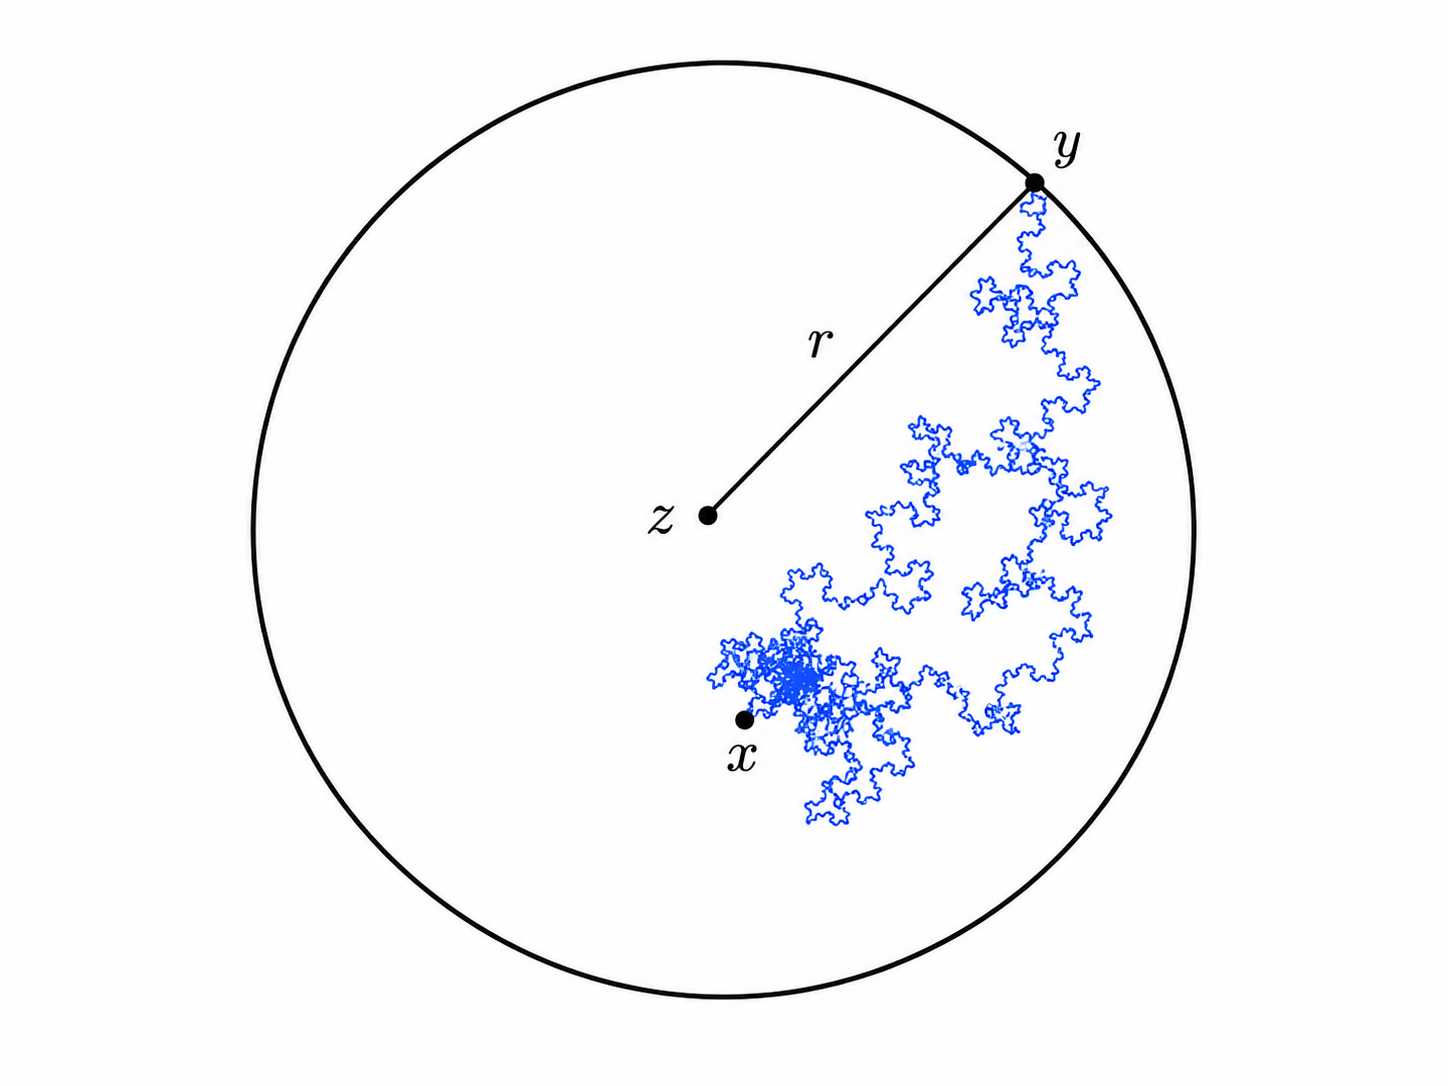
\includegraphics[height=200, alt="A ball with center z, a pole x inside it, and a Brownian path from x to a point y on the sphere"]{brownian_circle.png}
\end{center}
Ball $B_Z(r)$, uniform when $X=Z$:
$$d\omega^X(Y)=\frac{r^{n-2}(r^2-|X-Z|^2)}{|X-Y|^n}\,\frac{d\sigma(Y)}{\sigma(\partial B_Z(r))}$$
\columnbreak
\begin{center}
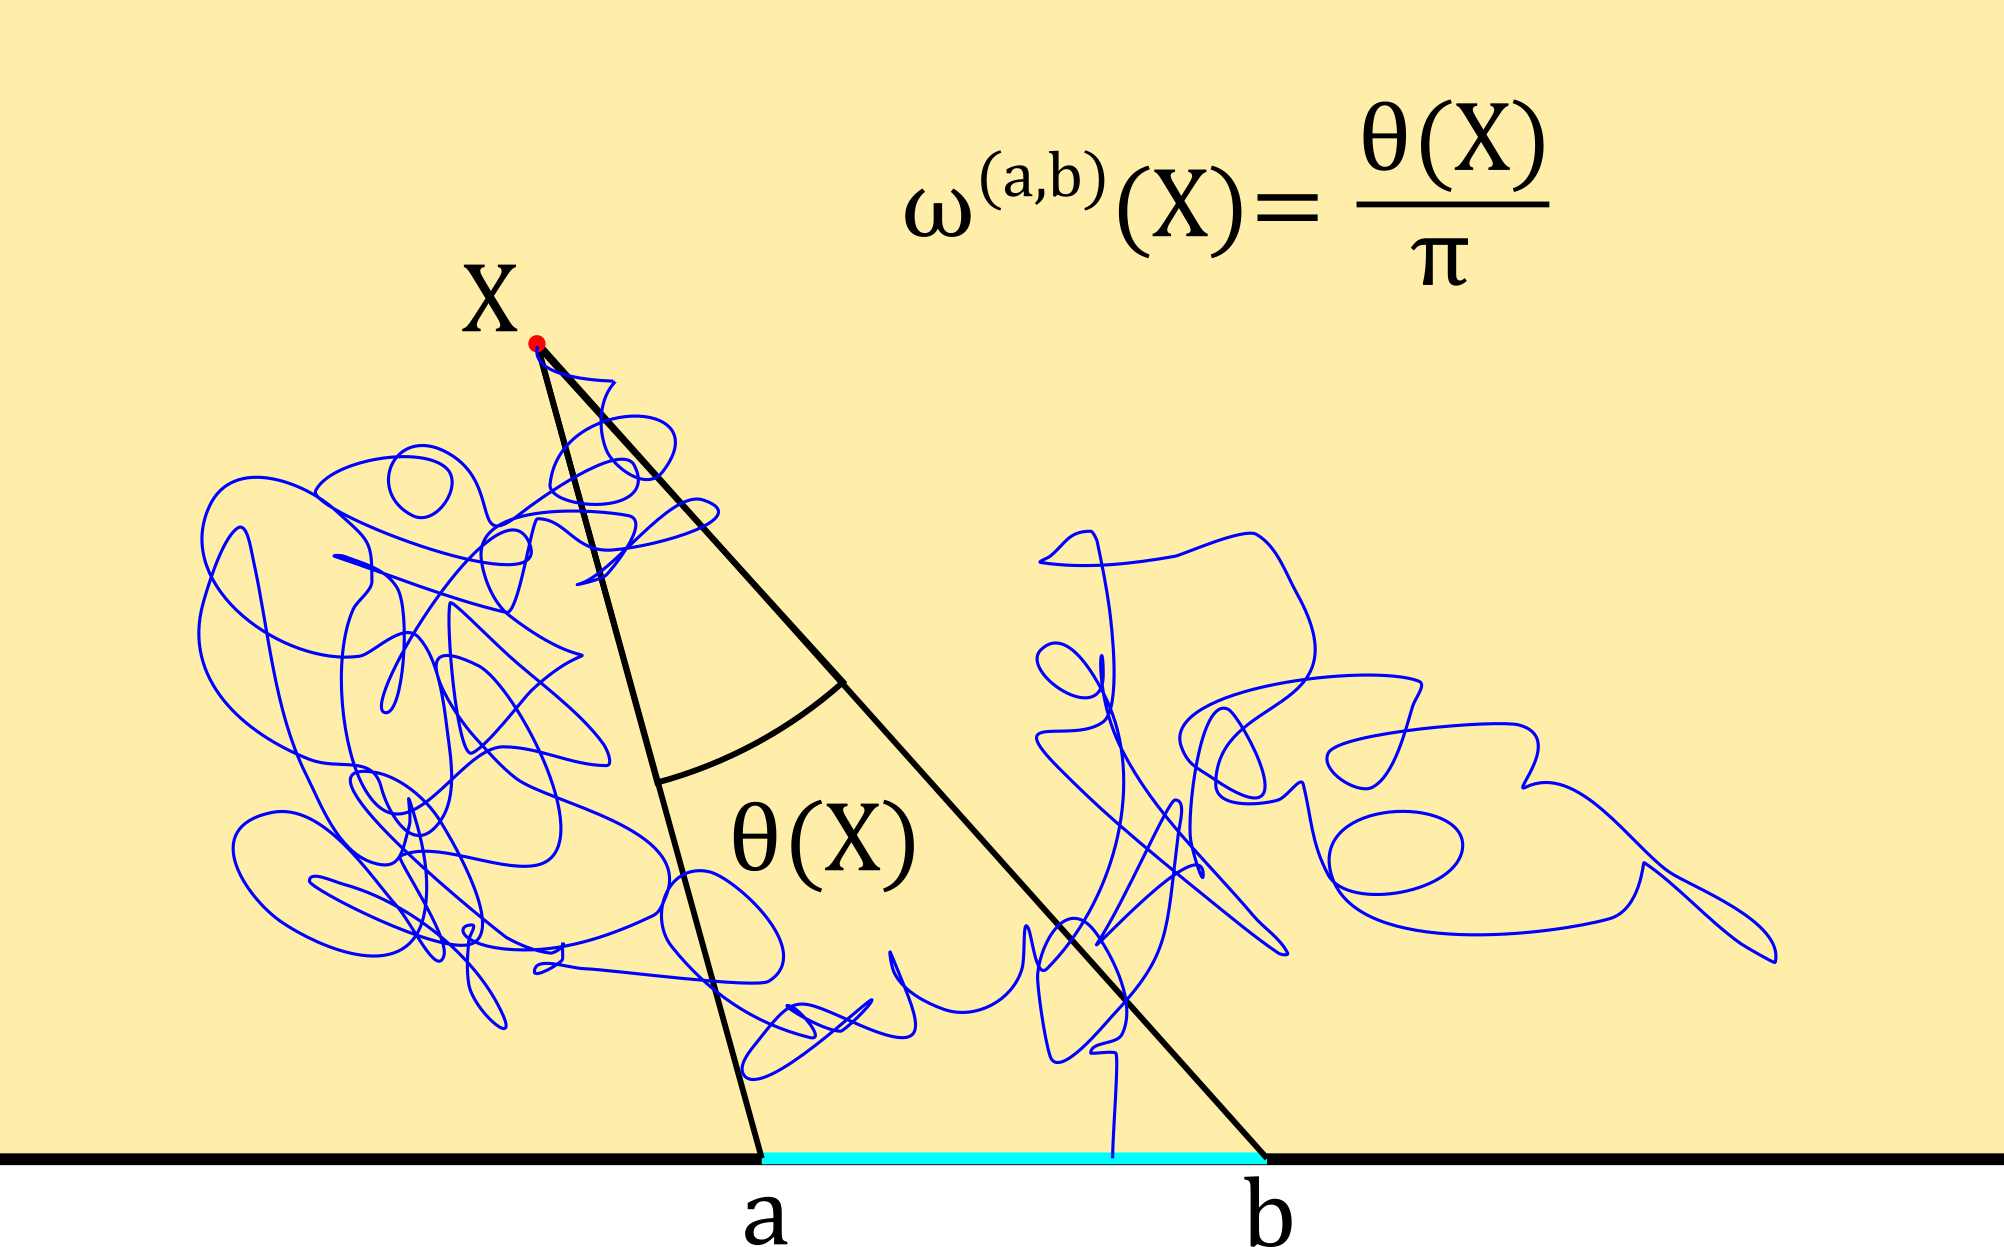
\includegraphics[height=200, alt="The upper half plane with an interval (a,b) on the axis and the angle theta(X) it subtends at a point X"]{anglefunction-hm.png}
\end{center}
Upper half plane:
$$\omega^X((a,b))=\frac{\theta(X)}{\pi}$$
\end{columns}

\slide{Harmonic measure is where Brownian motion exits}
\begin{columns}[8 5]
Start a random path (\textcolor{c3}{\textbf{Brownian motion}}) at $X\in\Omega$. It first leaves $\Omega$ at a random point $B_{\mathsf{exit}}\in\partial\Omega$, and
$$\textcolor{c3}{\omega^X(E)=\Prob(B_{\mathsf{exit}}\in E\mid B_0=X)}$$
\columnbreak
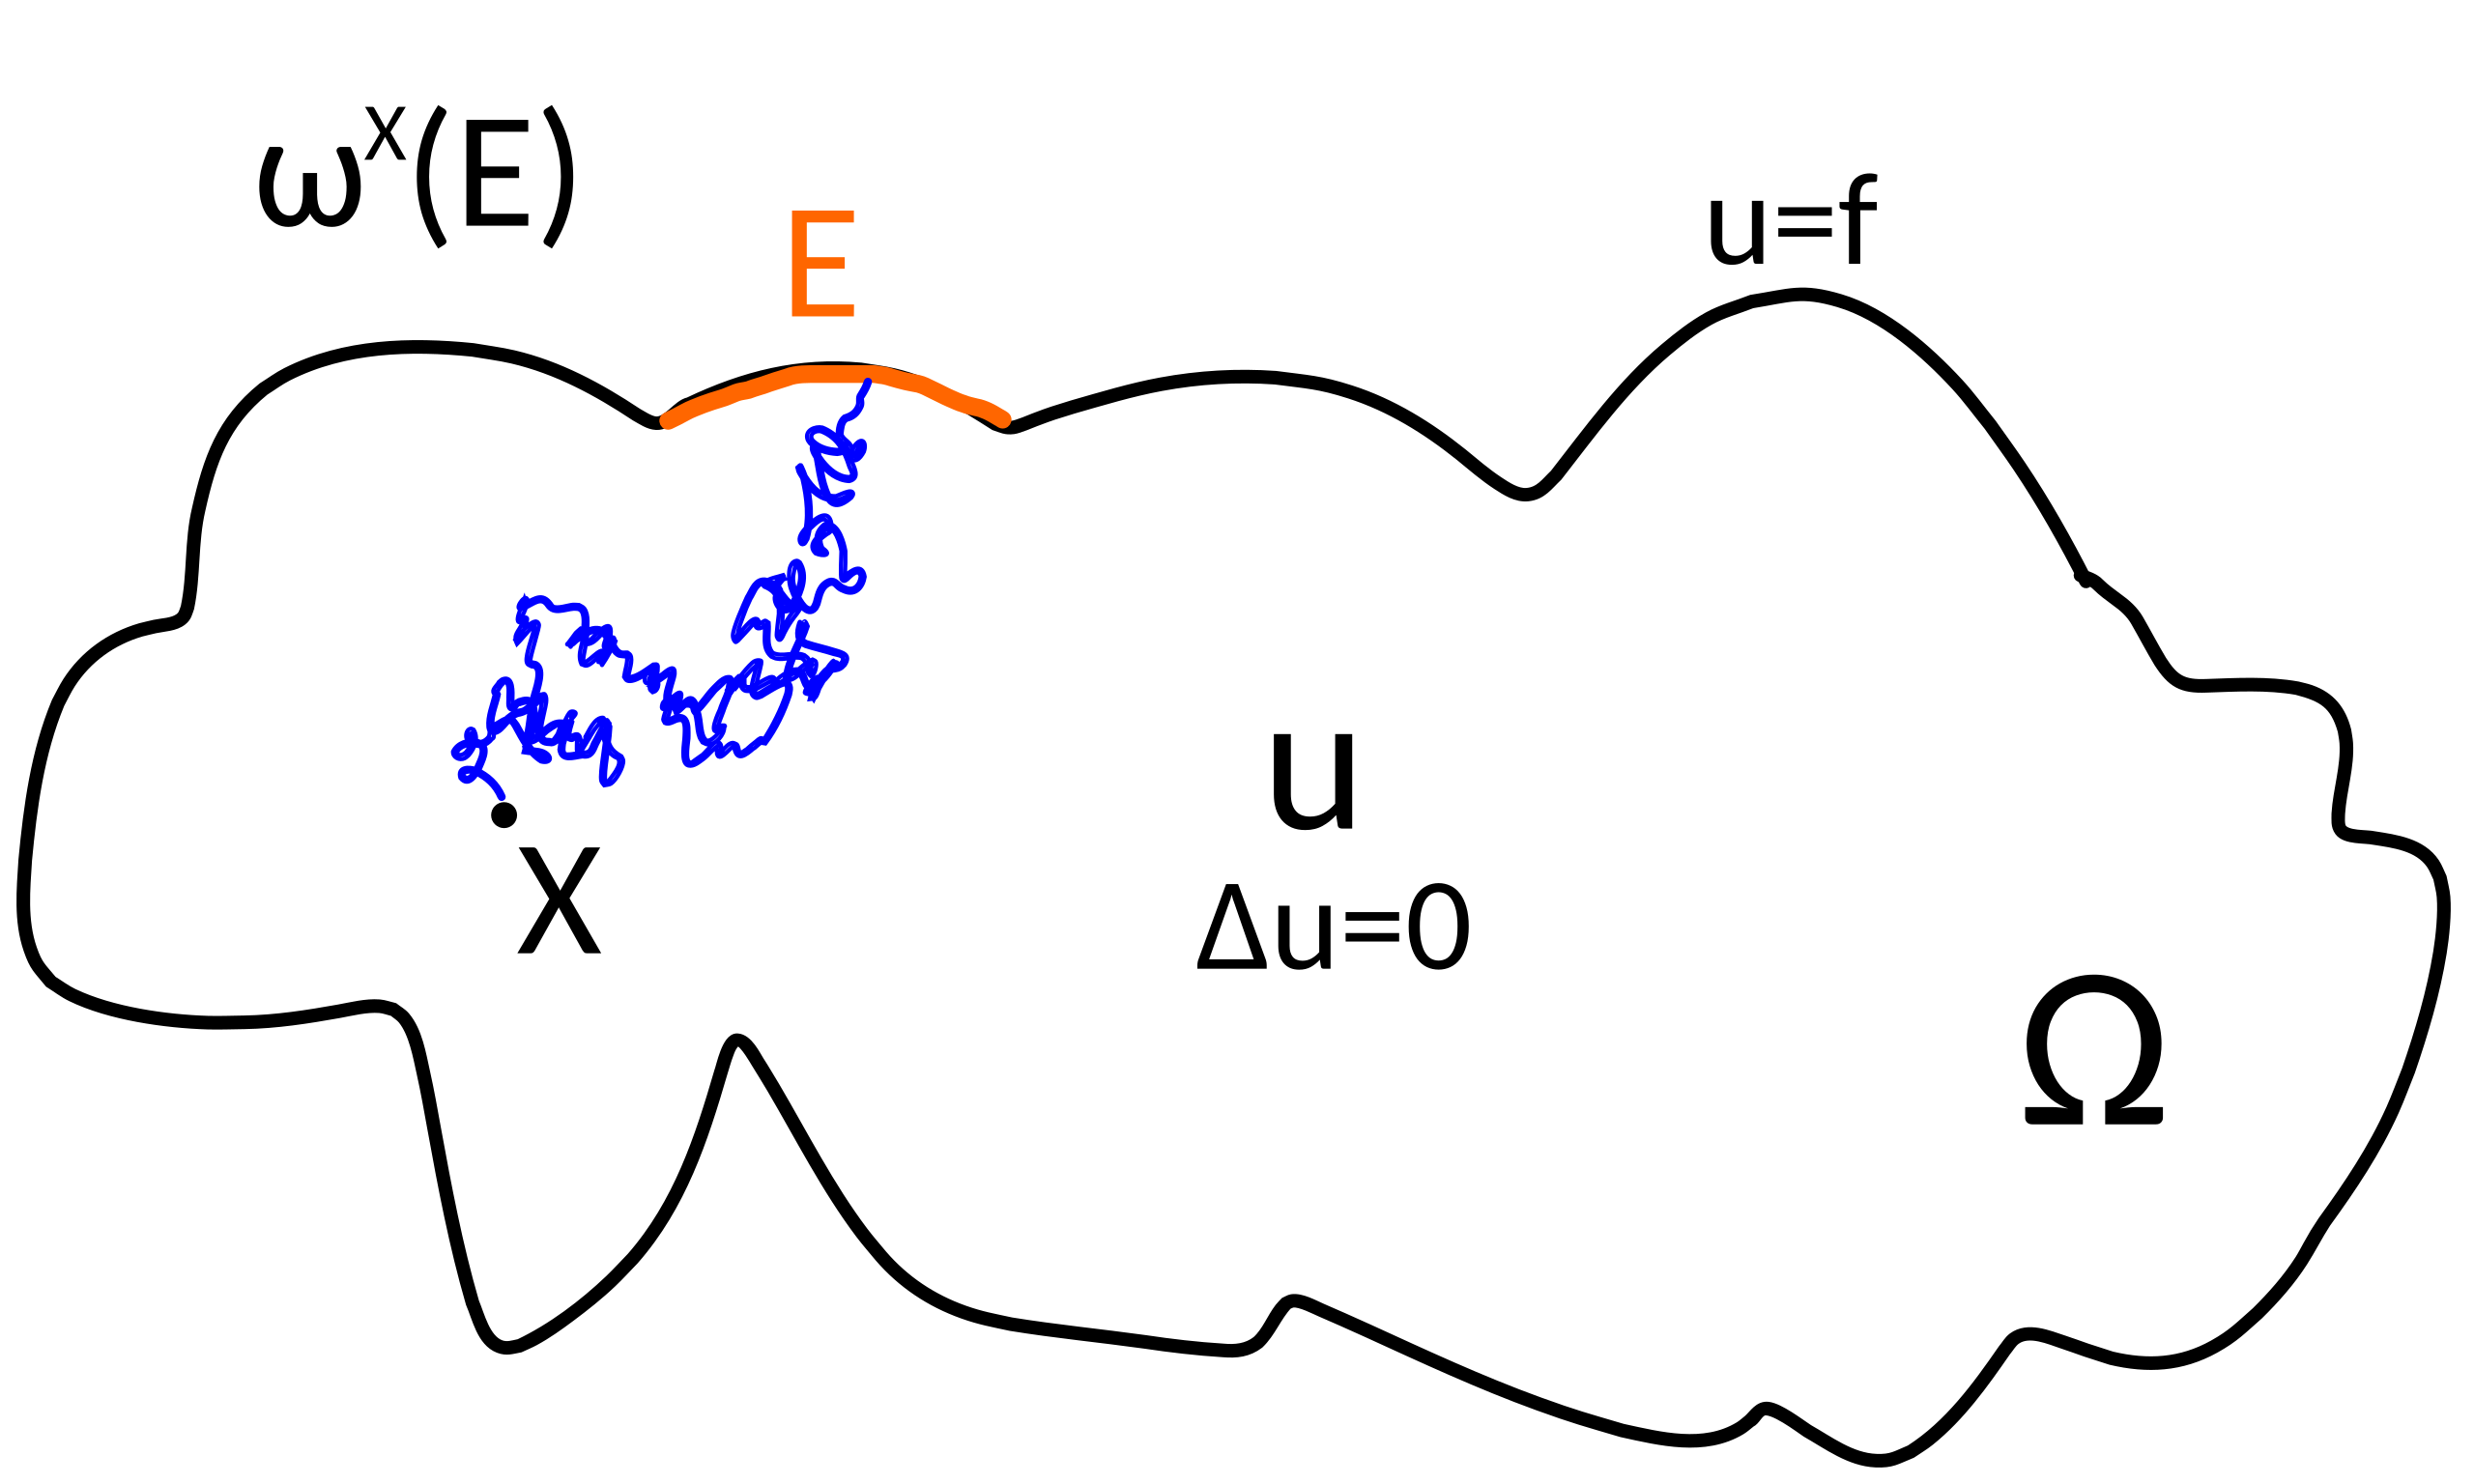
\includegraphics[width=560, alt="A domain Omega with a Brownian path from X that first hits the boundary in a set E, where u equals f"]{CloudDomain.png}
\end{columns}
\begin{itemize}
\item Started at the center of a ball, Brownian motion exits uniformly by symmetry. This is the mean value property!
\item \textbf{Dirichlet problem:} for boundary data $f$, the average $u_f(X)=\int f\,d\omega^X$ is harmonic in $\Omega$ and has boundary values $f$ \alert{except on a set of harmonic measure zero}
\item This is one reason to care about the null sets and the dimension of harmonic measure
\end{itemize}

\slide{Simulation: Brownian motion in a square}
\begin{js}[size=1640x680, frames=1, alt="Interactive: Brownian paths in a square, started at a point you click; exit points are colored by edge, or by middle thirds versus outer thirds, with running counts"]
const font = (k, b) => (b ? '600 ' : '') + k + "px 'JetBrains Mono', monospace";
const SQ = 620, OX = 30, OY = 30, TX = 760, TX1 = 1610; // the panel keeps counts for every path drawn or run
const PX = (x) => OX + x * SQ, PY = (y) => OY + (1 - y) * SQ;
const EDGE = ['bottom edge', 'right edge', 'top edge', 'left edge'];
const ECOL = [colors.c3, colors.c4, colors.c1, colors.c2];
const ZONE = ['middle thirds', 'outer thirds'], ZCOL = [colors.c4, colors.c1];
canvas.style.touchAction = 'none';
function reset() { state.c4 = [0, 0, 0, 0]; state.c2 = [0, 0]; state.n = 0; state.dots = []; state.path = null; state.queue = 0; }
if (state.mode === undefined) { state.mode = 0; state.sx = 0.5; state.sy = 0.5; reset(); }
let spare = null;
function gauss() {
  if (spare !== null) { const g = spare; spare = null; return g; }
  const u = 1 - Math.random(), v = Math.random(), r = Math.sqrt(-2 * Math.log(u));
  spare = r * Math.sin(2 * Math.PI * v); return r * Math.cos(2 * Math.PI * v);
}
// exit point (x, y) on the boundary: edge 0..3 (bottom, right, top, left) and coordinate t along it
function record(x, y) {
  const d = [y, 1 - x, 1 - y, x]; let e = 0; for (let k = 1; k < 4; k++) if (d[k] < d[e]) e = k;
  const t = (e === 0 || e === 2) ? x : y, mid = t > 1 / 3 && t < 2 / 3;
  state.c4[e]++; state.c2[mid ? 0 : 1]++; state.n++;
  state.dots.push([x, y, e, mid]); if (state.dots.length > 900) state.dots.shift();
}
// fast paths: Brownian motion sampled at times adapted to the distance d to the boundary,
// each increment exactly N(0, (0.2 d)^2 I), stopped within 1e-4 of the boundary
function fast() {
  let x = 0.5, y = 0.5;
  for (let i = 0; i < 100000; i++) {
    const d = Math.min(x, 1 - x, y, 1 - y);
    if (d < 1e-4) break;
    x += 0.2 * d * gauss(); y += 0.2 * d * gauss();
  }
  record(Math.min(1, Math.max(0, x)), Math.min(1, Math.max(0, y)));
}
// the drawn path: Gaussian steps of fixed size, cut where the last segment crosses the boundary
function advance() {
  const p = state.path; if (!p || p.done) return;
  for (let i = 0; i < 30; i++) {
    const [x, y] = p.pts[p.pts.length - 1];
    const nx = x + 0.006 * gauss(), ny = y + 0.006 * gauss();
    if (nx > 0 && nx < 1 && ny > 0 && ny < 1) { p.pts.push([nx, ny]); continue; }
    let t = 1;
    if (nx <= 0) t = Math.min(t, x / (x - nx)); if (nx >= 1) t = Math.min(t, (1 - x) / (nx - x));
    if (ny <= 0) t = Math.min(t, y / (y - ny)); if (ny >= 1) t = Math.min(t, (1 - y) / (ny - y));
    const ex = Math.min(1, Math.max(0, x + t * (nx - x))), ey = Math.min(1, Math.max(0, y + t * (ny - y)));
    p.pts.push([ex, ey]); p.done = true; record(ex, ey); return;
  }
}
const BTN = { e: [TX, 30, 300, 66], m: [TX + 330, 30, 360, 66], run: [TX, 560, 420, 66], clr: [TX + 450, 560, 200, 66] };
function button(b, label, on) {
  ctx.fillStyle = on ? colors.ink : '#ffffff'; ctx.strokeStyle = colors.ink; ctx.lineWidth = 3;
  ctx.beginPath(); ctx.roundRect(b[0], b[1], b[2], b[3], 33); ctx.fill(); ctx.stroke();
  ctx.fillStyle = on ? '#ffffff' : colors.ink; ctx.font = font(30, true); ctx.textAlign = 'center';
  ctx.fillText(label, b[0] + b[2] / 2, b[1] + 44);
}
function region(x, y, e, mid) { return state.mode === 0 ? ECOL[e] : ZCOL[mid ? 0 : 1]; }
function draw() {
  ctx.clearRect(0, 0, w, h);
  ctx.fillStyle = '#FBFAF4'; ctx.fillRect(OX, OY, SQ, SQ);
  ctx.lineWidth = 10; ctx.lineCap = 'butt';
  const seg = (x0, y0, x1, y1, c) => { ctx.strokeStyle = c; ctx.beginPath(); ctx.moveTo(PX(x0), PY(y0)); ctx.lineTo(PX(x1), PY(y1)); ctx.stroke(); };
  const ends = [[0, 0, 1, 0], [1, 0, 1, 1], [0, 1, 1, 1], [0, 0, 0, 1]];
  for (let e = 0; e < 4; e++) {
    const [x0, y0, x1, y1] = ends[e];
    if (state.mode === 0) seg(x0, y0, x1, y1, ECOL[e]);
    else for (let k = 0; k < 3; k++) seg(x0 + (x1 - x0) * k / 3, y0 + (y1 - y0) * k / 3, x0 + (x1 - x0) * (k + 1) / 3, y0 + (y1 - y0) * (k + 1) / 3, k === 1 ? ZCOL[0] : ZCOL[1]);
  }
  // recent exit points, drawn just outside the square
  for (const [x, y, e, mid] of state.dots) {
    const ox = e === 1 ? 16 : e === 3 ? -16 : 0, oy = e === 0 ? 16 : e === 2 ? -16 : 0;
    ctx.fillStyle = region(x, y, e, mid); ctx.globalAlpha = 0.55;
    ctx.beginPath(); ctx.arc(PX(x) + ox + (Math.random() - 0.5) * 0, PY(y) + oy, 4, 0, 2 * Math.PI); ctx.fill();
  }
  ctx.globalAlpha = 1;
  const p = state.path;
  if (p) {
    ctx.strokeStyle = 'rgba(30,42,56,0.85)'; ctx.lineWidth = 2; ctx.lineJoin = 'round';
    ctx.beginPath(); p.pts.forEach((q, i) => i ? ctx.lineTo(PX(q[0]), PY(q[1])) : ctx.moveTo(PX(q[0]), PY(q[1]))); ctx.stroke();
    if (p.done) { const q = p.pts[p.pts.length - 1], d = state.dots[state.dots.length - 1]; ctx.fillStyle = region(q[0], q[1], d[2], d[3]); ctx.beginPath(); ctx.arc(PX(q[0]), PY(q[1]), 12, 0, 2 * Math.PI); ctx.fill(); }
  }
  ctx.fillStyle = colors.alert; ctx.beginPath(); ctx.arc(PX(state.sx), PY(state.sy), 10, 0, 2 * Math.PI); ctx.fill();
  button(BTN.e, 'four edges', state.mode === 0); button(BTN.m, 'middle thirds', state.mode === 1);
  const n = state.n, rows = state.mode === 0 ? EDGE.map((l, k) => [l, state.c4[k], ECOL[k]]) : ZONE.map((l, k) => [l, state.c2[k], ZCOL[k]]);
  let y = 190;
  for (const [label, c, col] of rows) {
    ctx.fillStyle = col; ctx.fillRect(TX, y - 30, 34, 34);
    ctx.fillStyle = colors.ink; ctx.textAlign = 'left'; ctx.font = font(32); ctx.fillText(label, TX + 54, y);
    const f = n ? c / n : 0, se = n ? 2 * Math.sqrt(f * (1 - f) / n) : 0;
    ctx.textAlign = 'right'; ctx.font = font(32, true); ctx.fillText(String(c), TX + 560, y);
    ctx.fillStyle = col; ctx.fillText(n ? (100 * f).toFixed(1) + '%' : '', TX1 - 150, y);
    ctx.font = font(24); ctx.fillStyle = colors.muted; ctx.fillText(n > 30 ? '± ' + (100 * se).toFixed(1) : '', TX1, y);
    y += 70;
  }
  ctx.textAlign = 'left'; ctx.fillStyle = colors.ink; ctx.font = font(30);
  ctx.fillText('paths: ' + n, TX, state.mode === 0 ? 490 : 350);
  button(BTN.run, state.queue > 0 ? 'running…' : '+1000 from center', false); button(BTN.clr, 'reset', false);
  ctx.fillStyle = colors.muted; ctx.font = font(24); ctx.textAlign = 'left';
  ctx.fillText('click in the square to start a path; the counts add up', TX, 670);
}
function pos(e) { const b = canvas.getBoundingClientRect(); return [(e.clientX - b.left) * w / b.width, (e.clientY - b.top) * h / b.height]; }
const inB = (b, x, y) => x >= b[0] && x <= b[0] + b[2] && y >= b[1] && y <= b[1] + b[3];
canvas.onpointerdown = (e) => {
  const [x, y] = pos(e);
  if (x > OX && x < OX + SQ && y > OY && y < OY + SQ) {
    state.sx = (x - OX) / SQ; state.sy = 1 - (y - OY) / SQ;
    state.path = { pts: [[state.sx, state.sy]], done: false };
  } else if (inB(BTN.e, x, y)) { if (state.mode !== 0) { state.mode = 0; reset(); } }
  else if (inB(BTN.m, x, y)) { if (state.mode !== 1) { state.mode = 1; reset(); } }
  else if (inB(BTN.run, x, y)) state.queue += 1000;
  else if (inB(BTN.clr, x, y)) { reset(); }
  else return;
  e.stopPropagation();
};
canvas.onclick = (e) => e.stopPropagation();
onFrame(() => {
  advance();
  const t0 = performance.now();
  while (state.queue > 0 && performance.now() - t0 < 12) { fast(); state.queue--; }
  draw();
});
\end{js}
\begin{center}
Started at the center, does Brownian motion leave more often through the \textcolor{c4}{middle thirds} of the edges or through the \textcolor{c1}{outer thirds}?
\end{center}

\slide{The middle thirds win, narrowly}
Let $E$ be the union of the \textcolor{c4}{middle thirds} of the four edges of the unit square
\medskip
Separation of variables gives a Fourier sine series for the harmonic measure:
$$\begin{aligned}\textcolor{c3}{\omega^{\text{center}}(E)}&=4\sum_{n=1}^\infty\frac{2}{n\pi}\,\frac{\sinh(n\pi/2)}{\sinh(n\pi)}\Big(\cos\frac{n\pi}{3}-\cos\frac{2n\pi}{3}\Big)\sin\frac{n\pi}{2}\\&=\alert{0.522873\ldots}\end{aligned}$$
\begin{center}
The middle thirds are $1/3$ of the length but catch more than half of the paths
\end{center}

\slide{Simulation: Brownian motion in a cube}
\begin{js}[size=1640x700, frames=1, alt="Interactive: Brownian paths in a cube drawn in three dimensions; the faces are colored by how often paths exit there, with a slider moving the starting point from the center toward a corner; drag to rotate"]
const font = (k, b) => (b ? '600 ' : '') + k + "px 'JetBrains Mono', monospace";
const CX = 350, CY = 360, SCL = 380, TX = 780, TX1 = 1610, SY = 110, G = 16;
canvas.style.touchAction = 'none';
if (state.yaw === undefined) { state.yaw = 0.62; state.pitch = 0.42; state.auto = true; state.t = 0; reset(); }
function reset() {
  state.cells = Array.from({ length: 6 }, () => new Float64Array(G * G)); state.face = [0, 0, 0, 0, 0, 0];
  state.n = 0; state.edge = 0; state.path = null; state.last = null; state.wait = 0;
}
const start = () => { const s = 0.5 + 0.42 * state.t; return [s, s, s]; };
let spare = null;
function gauss() {
  if (spare !== null) { const g = spare; spare = null; return g; }
  const u = 1 - Math.random(), v = Math.random(), r = Math.sqrt(-2 * Math.log(u));
  spare = r * Math.sin(2 * Math.PI * v); return r * Math.cos(2 * Math.PI * v);
}
// faces 0..5: x = 0, x = 1, y = 0, y = 1, z = 0, z = 1
function record(p) {
  const d = [p[0], 1 - p[0], p[1], 1 - p[1], p[2], 1 - p[2]];
  let f = 0; for (let k = 1; k < 6; k++) if (d[k] < d[f]) f = k;
  const a = f >> 1, b = (a + 1) % 3, c = (a + 2) % 3;
  const i = Math.min(G - 1, Math.floor(p[b] * G)), j = Math.min(G - 1, Math.floor(p[c] * G));
  state.cells[f][i * G + j]++; state.face[f]++; state.n++;
  const near = Math.min(p[b], 1 - p[b], p[c], 1 - p[c]); if (near < 0.01) state.edge++;
  return f;
}
// fast paths: increments exactly N(0, (0.2 d)^2 I), d = distance to the boundary, stopped within 1e-4
function fast() {
  const p = start();
  for (let i = 0; i < 100000; i++) {
    const d = Math.min(p[0], 1 - p[0], p[1], 1 - p[1], p[2], 1 - p[2]);
    if (d < 1e-4) break;
    const s = 0.2 * d; p[0] += s * gauss(); p[1] += s * gauss(); p[2] += s * gauss();
  }
  record(p.map((v) => Math.min(1, Math.max(0, v))));
}
// the drawn path: Gaussian steps of fixed size, cut where the last segment crosses the boundary
function advance() {
  if (!state.path) { if (state.wait-- > 0) return; state.path = { pts: [start()], done: false }; }
  const P = state.path;
  for (let i = 0; i < 40 && !P.done; i++) {
    const q = P.pts[P.pts.length - 1], r = [q[0] + 0.007 * gauss(), q[1] + 0.007 * gauss(), q[2] + 0.007 * gauss()];
    let t = 1;
    for (let k = 0; k < 3; k++) { if (r[k] <= 0) t = Math.min(t, q[k] / (q[k] - r[k])); if (r[k] >= 1) t = Math.min(t, (1 - q[k]) / (r[k] - q[k])); }
    if (t === 1) { P.pts.push(r); continue; }
    const e = q.map((v, k) => Math.min(1, Math.max(0, v + t * (r[k] - v))));
    P.pts.push(e); P.done = true; P.face = record(e);
  }
  if (P.done) { state.last = P; state.path = null; state.wait = 25; }
}
function view(p) {
  const qx = p[0] - 0.5, qy = p[1] - 0.5, qz = p[2] - 0.5, cy = Math.cos(state.yaw), sy = Math.sin(state.yaw);
  const x1 = qx * cy - qy * sy, y1 = qx * sy + qy * cy, cp = Math.cos(state.pitch), sp = Math.sin(state.pitch);
  const depth = y1 * cp - qz * sp, up = y1 * sp + qz * cp, f = 3.2 / (3.2 + depth);
  return [CX + SCL * f * x1, CY - SCL * f * up, depth];
}
function faceDepthSign(f) {
  // the face is toward the viewer when its outward normal points against the viewing direction
  const a = f >> 1, s = (f & 1) ? 1 : -1, n = [0, 0, 0]; n[a] = s;
  const cy = Math.cos(state.yaw), sy = Math.sin(state.yaw);
  const y1 = n[0] * sy + n[1] * cy, depth = y1 * Math.cos(state.pitch) - n[2] * Math.sin(state.pitch);
  return depth < 0;
}
function heat(v) {
  // pale to purple to dark purple
  const st = [[244, 238, 246], [196, 150, 196], [142, 58, 138], [70, 20, 68]];
  const x = Math.min(0.999, Math.max(0, v)) * (st.length - 1), i = Math.floor(x), u = x - i;
  return 'rgb(' + [0, 1, 2].map((k) => Math.round(st[i][k] * (1 - u) + st[i + 1][k] * u)).join(',') + ')';
}
function drawFace(f, alpha) {
  const a = f >> 1, b = (a + 1) % 3, c = (a + 2) % 3, val = (f & 1) ? 1 : 0;
  let mx = 0; for (const cs of state.cells) for (const v of cs) mx = Math.max(mx, v);
  ctx.globalAlpha = alpha;
  for (let i = 0; i < G; i++) for (let j = 0; j < G; j++) {
    const corner = (di, dj) => { const p = [0, 0, 0]; p[a] = val; p[b] = (i + di) / G; p[c] = (j + dj) / G; return view(p); };
    const P = [corner(0, 0), corner(1, 0), corner(1, 1), corner(0, 1)];
    const v = mx ? Math.sqrt(state.cells[f][i * G + j] / mx) : 0;
    ctx.fillStyle = heat(v); ctx.strokeStyle = ctx.fillStyle; ctx.lineWidth = 1;
    ctx.beginPath(); P.forEach((q, k) => k ? ctx.lineTo(q[0], q[1]) : ctx.moveTo(q[0], q[1])); ctx.closePath(); ctx.fill(); ctx.stroke();
  }
  ctx.globalAlpha = 1;
}
function edges(front) {
  const V = [];
  for (let k = 0; k < 8; k++) V.push(view([k & 1, (k >> 1) & 1, (k >> 2) & 1]));
  ctx.strokeStyle = colors.ink; ctx.lineWidth = front ? 3 : 1.5; ctx.setLineDash(front ? [] : [8, 8]);
  for (let k = 0; k < 8; k++) for (const m of [1, 2, 4]) if (!(k & m)) {
    // an edge is in front when either face through it faces the viewer
    const fa = [], bits = [1, 2, 4].filter((x) => x !== m);
    for (const bt of bits) { const ax = [1, 2, 4].indexOf(bt); fa.push(2 * ax + ((k & bt) ? 1 : 0)); }
    const isFront = fa.some(faceDepthSign);
    if (isFront !== front) continue;
    ctx.beginPath(); ctx.moveTo(V[k][0], V[k][1]); ctx.lineTo(V[k | m][0], V[k | m][1]); ctx.stroke();
  }
  ctx.setLineDash([]);
}
function path(P, alpha) {
  if (!P) return;
  ctx.strokeStyle = 'rgba(30,42,56,' + alpha + ')'; ctx.lineWidth = 2; ctx.lineJoin = 'round';
  ctx.beginPath(); P.pts.forEach((q, i) => { const v = view(q); i ? ctx.lineTo(v[0], v[1]) : ctx.moveTo(v[0], v[1]); }); ctx.stroke();
}
function draw() {
  ctx.clearRect(0, 0, w, h);
  const back = [0, 1, 2, 3, 4, 5].filter((f) => !faceDepthSign(f)), front = [0, 1, 2, 3, 4, 5].filter(faceDepthSign);
  back.forEach((f) => drawFace(f, 1)); edges(false);
  path(state.last, state.path ? 0.25 : 0.8); path(state.path, 0.85);
  const s = view(start()); ctx.fillStyle = colors.alert; ctx.beginPath(); ctx.arc(s[0], s[1], 9, 0, 2 * Math.PI); ctx.fill();
  if (state.last && !state.path) { const e = view(state.last.pts[state.last.pts.length - 1]); ctx.fillStyle = colors.c3; ctx.beginPath(); ctx.arc(e[0], e[1], 11, 0, 2 * Math.PI); ctx.fill(); }
  front.forEach((f) => drawFace(f, 0.22)); edges(true);
  // panel
  ctx.fillStyle = colors.ink; ctx.font = font(32); ctx.textAlign = 'left';
  ctx.fillText(state.t < 0.01 ? 'start point: the center' : 'start point: toward a corner', TX, SY - 36);
  ctx.strokeStyle = colors.grid; ctx.lineWidth = 10; ctx.lineCap = 'round'; ctx.beginPath(); ctx.moveTo(TX, SY); ctx.lineTo(TX1, SY); ctx.stroke();
  const sx = TX + state.t * (TX1 - TX);
  ctx.strokeStyle = colors.alert; ctx.beginPath(); ctx.moveTo(TX, SY); ctx.lineTo(sx, SY); ctx.stroke();
  ctx.fillStyle = colors.alert; ctx.beginPath(); ctx.arc(sx, SY, 17, 0, 2 * Math.PI); ctx.fill();
  const n = state.n, lab = ['x = 0', 'x = 1', 'y = 0', 'y = 1', 'z = 0', 'z = 1'];
  ctx.font = font(30); ctx.fillStyle = colors.ink; ctx.fillText('exits through each face, from ' + n + ' paths', TX, 220);
  for (let f = 0; f < 6; f++) {
    const x = TX + (f % 3) * 280, y = 285 + Math.floor(f / 3) * 62;
    ctx.fillStyle = colors.muted; ctx.font = font(28); ctx.fillText(lab[f], x, y);
    ctx.fillStyle = colors.c3; ctx.font = font(32, true); ctx.fillText(n ? (100 * state.face[f] / n).toFixed(1) + '%' : '…', x + 120, y);
  }
  ctx.fillStyle = colors.ink; ctx.font = font(30); ctx.fillText('exits within 0.01 of an edge', TX, 470);
  ctx.fillStyle = colors.c1; ctx.font = font(40, true); ctx.fillText(n ? (100 * state.edge / n).toFixed(2) + '%' : '…', TX, 525);
  ctx.fillStyle = colors.muted; ctx.font = font(24); ctx.fillText('those strips cover 3.96% of the surface area', TX, 565);
  for (let k = 0; k <= 20; k++) { ctx.fillStyle = heat(k / 20); ctx.fillRect(TX + k * 22, 610, 22, 26); }
  ctx.fillStyle = colors.muted; ctx.font = font(24); ctx.fillText('rarely hit', TX, 670); ctx.textAlign = 'right'; ctx.fillText('often hit', TX + 462, 670);
  ctx.textAlign = 'left'; ctx.fillText('drag the cube to rotate it', TX + 520, 640);
}
function pos(e) { const b = canvas.getBoundingClientRect(); return [(e.clientX - b.left) * w / b.width, (e.clientY - b.top) * h / b.height]; }
let drag = null;
canvas.onpointerdown = (e) => {
  const [x, y] = pos(e);
  if (Math.abs(y - SY) < 40 && x > TX - 30) drag = { k: 'slider' };
  else if (x < 720) drag = { k: 'rot', x: x, y: y, yaw: state.yaw, pitch: state.pitch };
  else return;
  state.auto = false; e.stopPropagation(); canvas.setPointerCapture(e.pointerId); move(x, y);
};
function move(x, y) {
  if (!drag) return;
  if (drag.k === 'slider') { const t = Math.round(Math.min(1, Math.max(0, (x - TX) / (TX1 - TX))) * 20) / 20; if (t !== state.t) { state.t = t; reset(); } }
  else { state.yaw = drag.yaw + (x - drag.x) * 0.008; state.pitch = Math.max(-1.2, Math.min(1.2, drag.pitch + (y - drag.y) * 0.008)); }
}
canvas.onpointermove = (e) => { if (drag) { const p = pos(e); move(p[0], p[1]); } };
canvas.onpointerup = canvas.onpointercancel = () => { drag = null; };
canvas.onclick = (e) => e.stopPropagation();
onFrame(() => {
  if (state.auto) state.yaw += 0.003;
  advance();
  const t0 = performance.now();
  while (performance.now() - t0 < 8 && state.n < 400000) fast();
  draw();
});
\end{js}
\begin{center}
Brownian motion almost never lands on an \textcolor{c1}{edge}, and from the center each face gets $1/6$
\end{center}

\slide{Physical interpretations}
\textcolor{c3}{\textbf{Diffusion}} is the net movement of molecules from regions of higher concentration to regions of lower concentration
\medskip
\textcolor{c3}{\textbf{Brownian motion}} models the trajectory of a single molecule undergoing diffusion
\medskip
\heading{Physical phenomena controlled by diffusion}
\begin{itemize}
\item heat transfer
\item electric charge on a metallic surface
\item passivation, fouling, poisoning, restricted absorption
\item transfer of nutrients from the digestive system to the blood
\item transfer of oxygen from air to blood during respiration
\end{itemize}

\slide{Passivation of irregular surfaces (Filoche et al.)}
\begin{columns}[4 6]
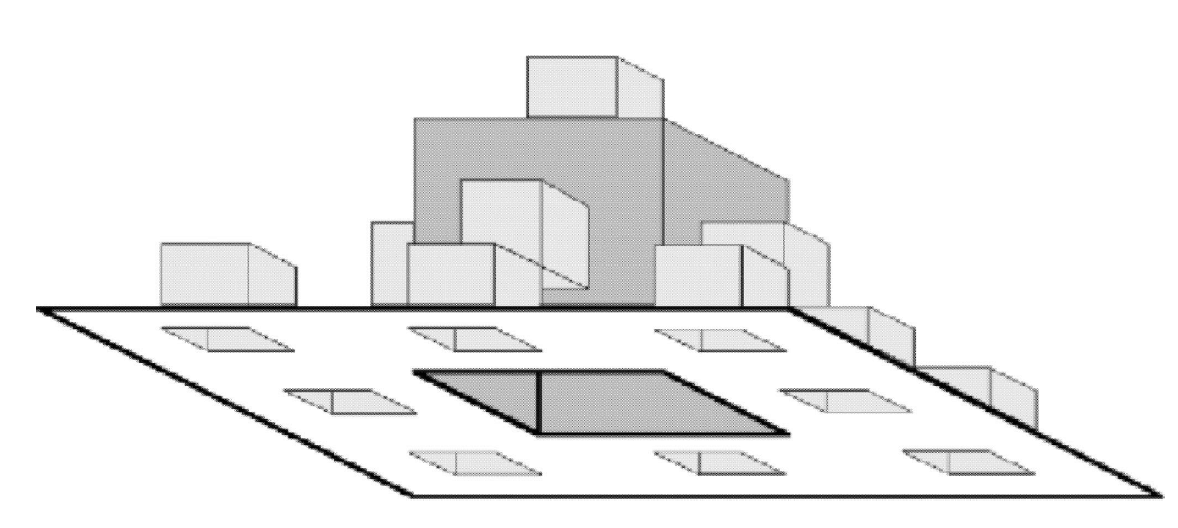
\includegraphics[width=560, alt="The generator of the cubic von Koch surface: a square face with a cube pushed out of its middle, and smaller cubes pushed out of each new face"]{cubical2.png}
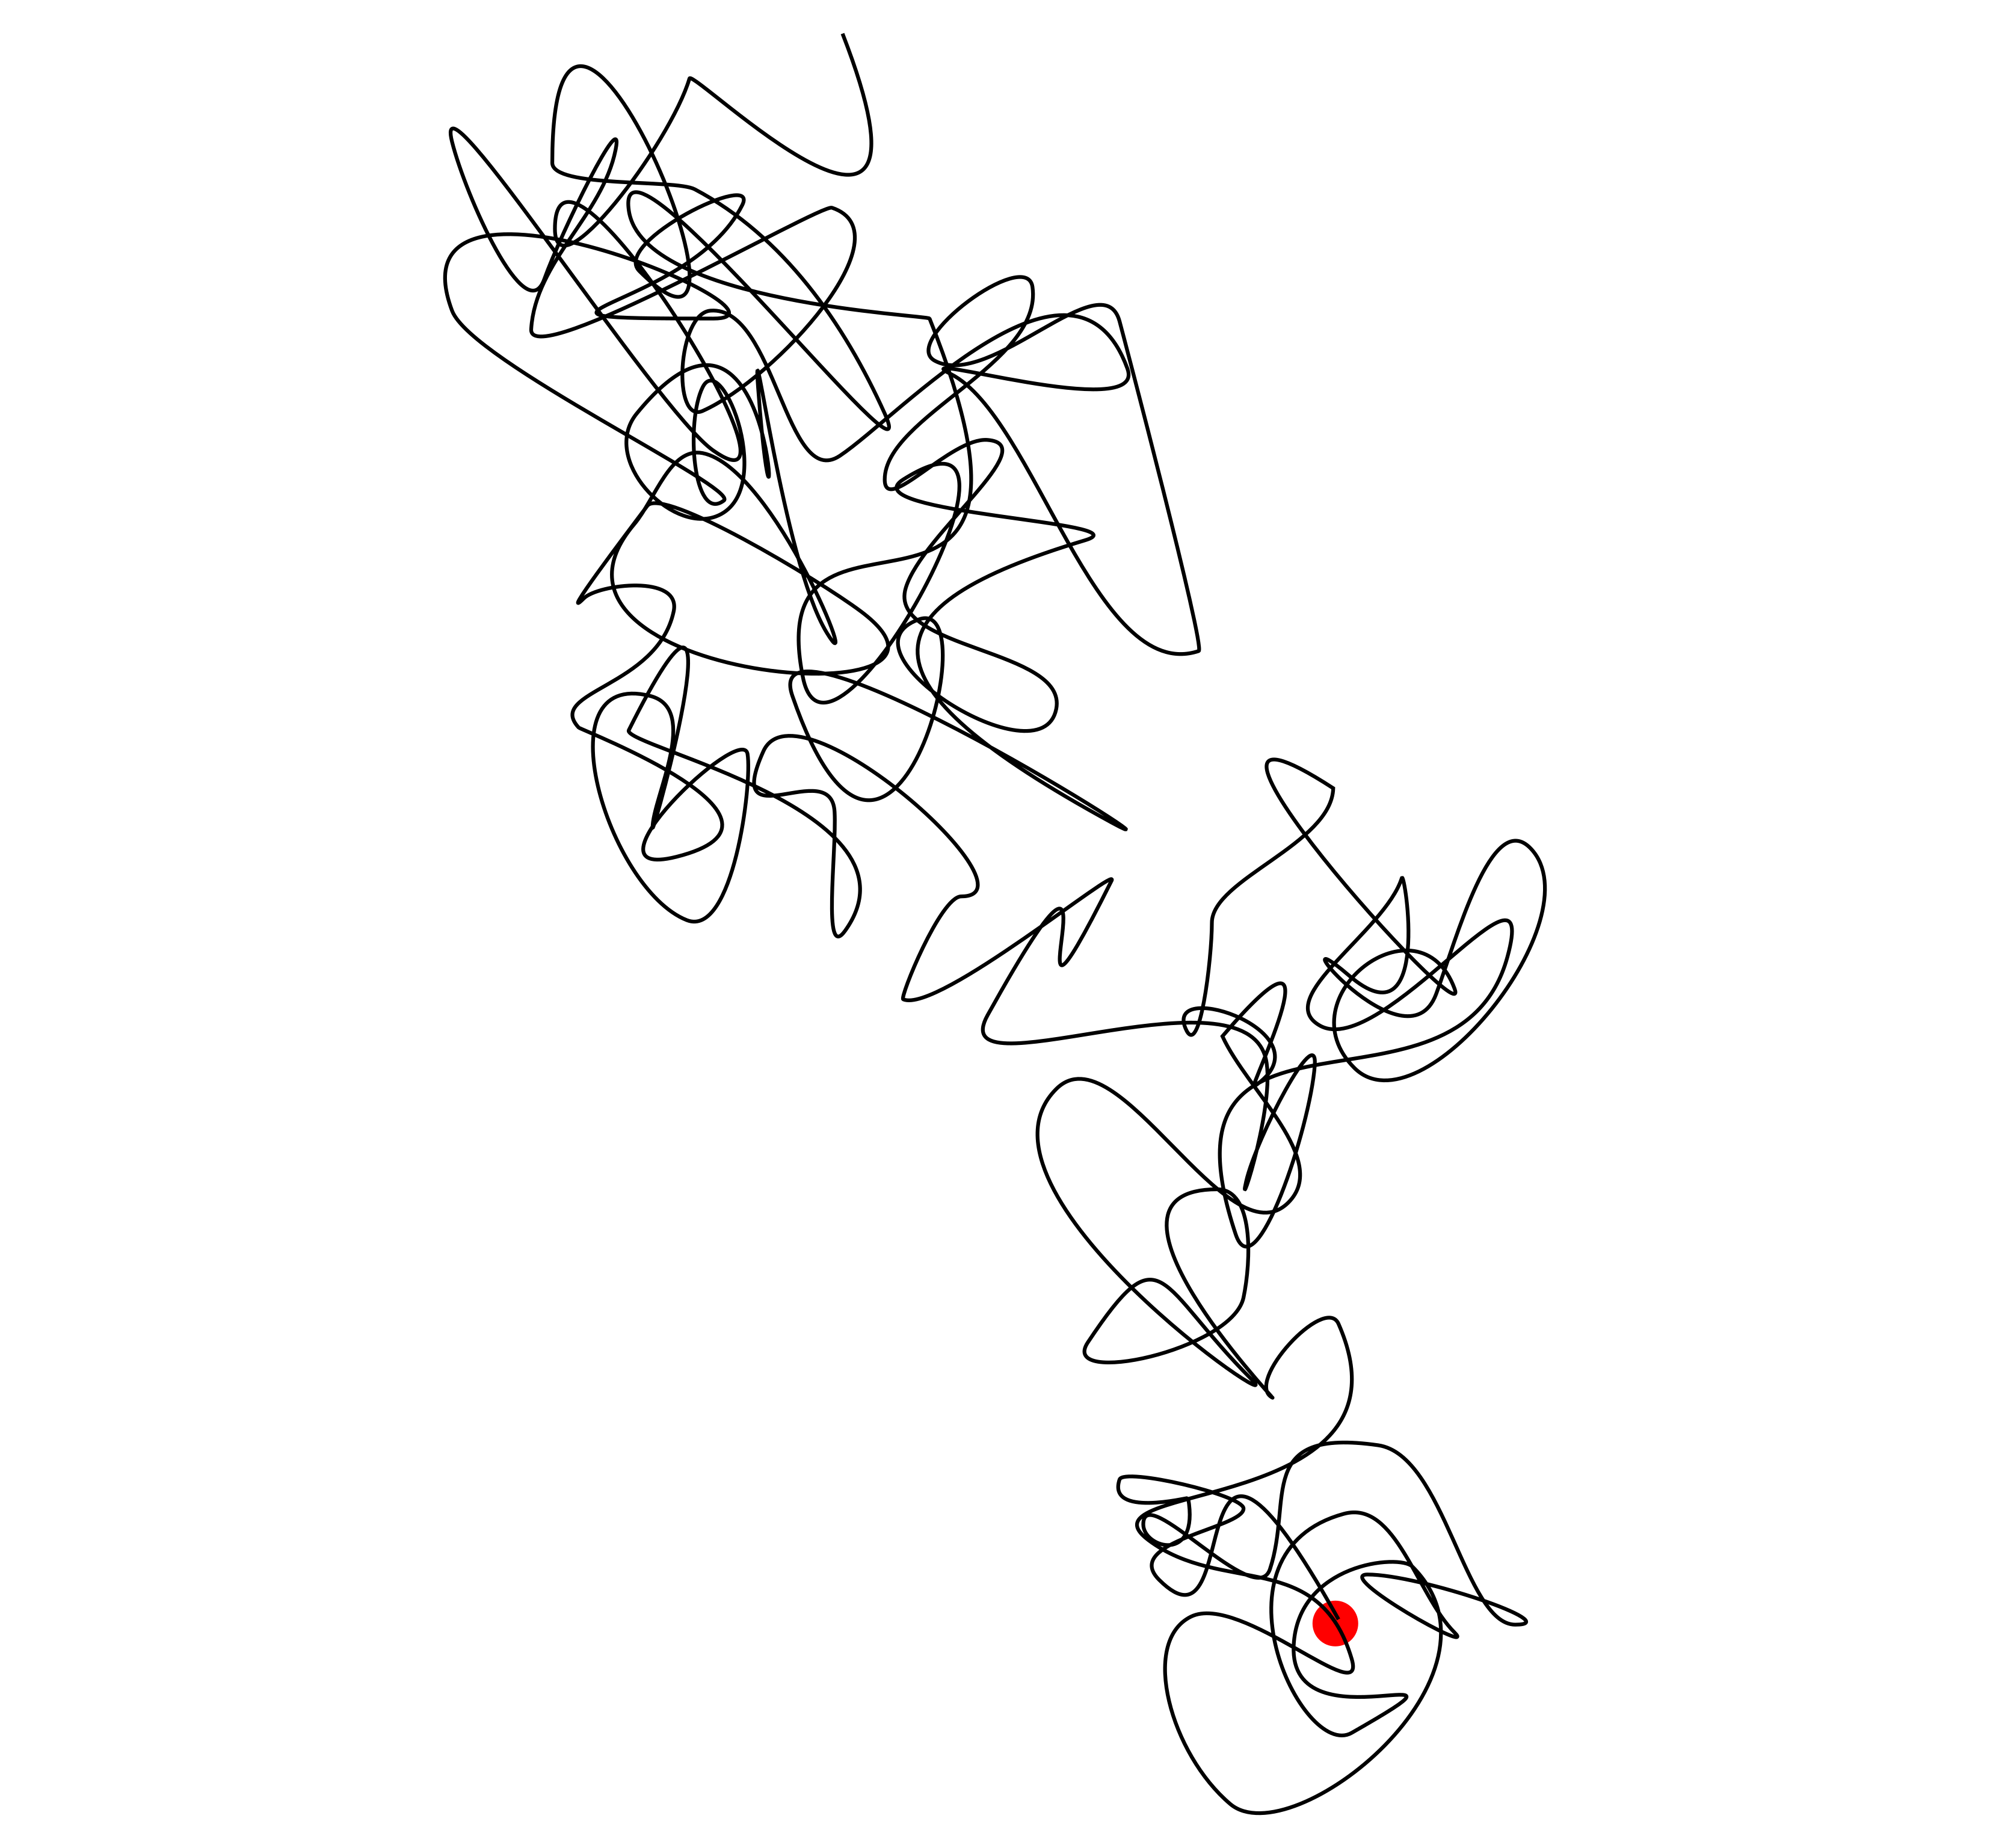
\includegraphics[width=330, alt="A random path rising from below toward the surface"]{upward_random_path.png}
\columnbreak
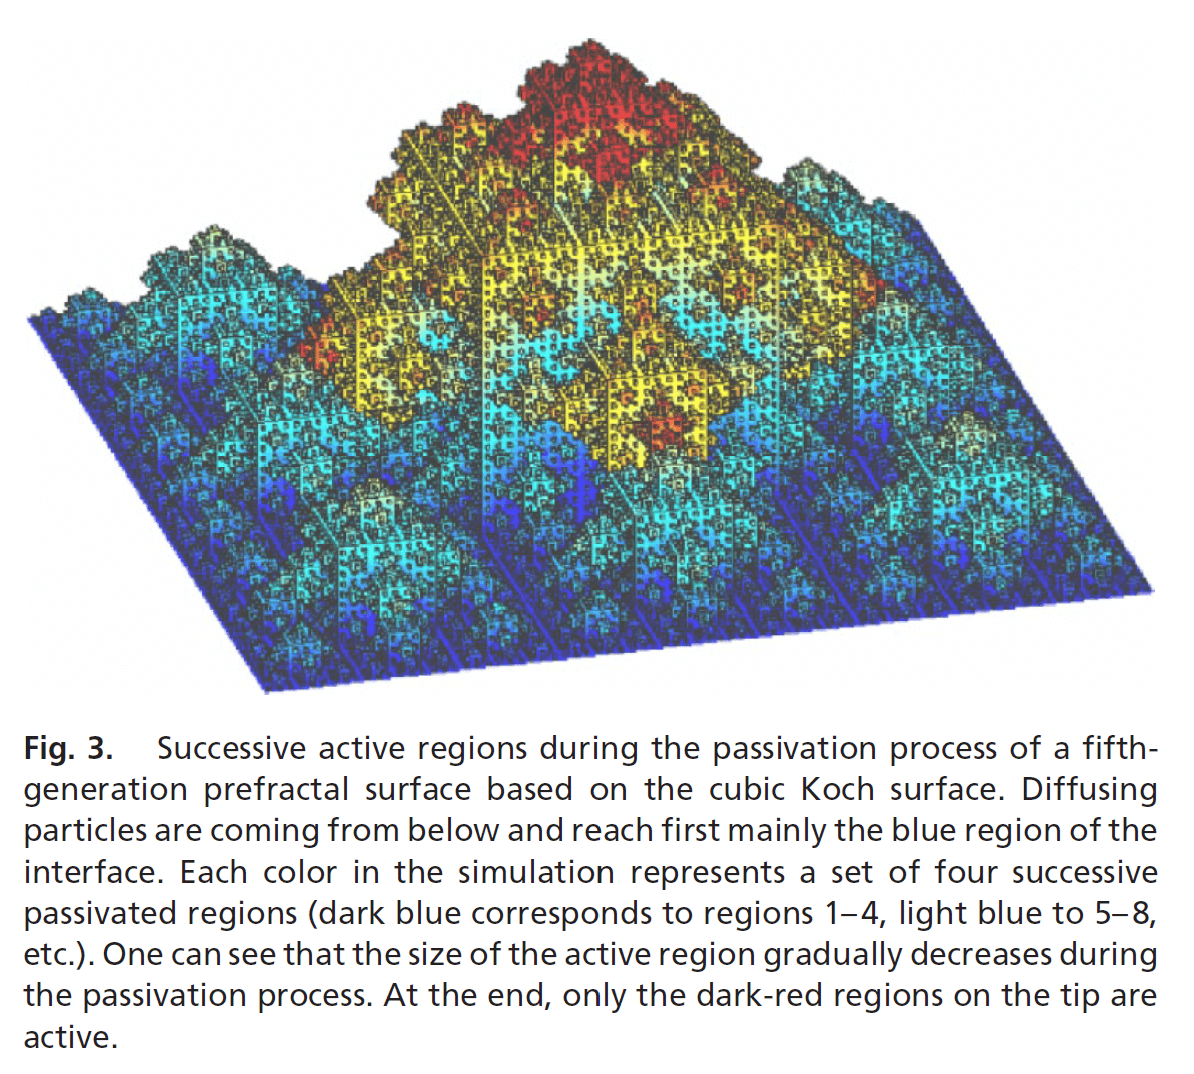
\includegraphics[height=700, alt="Successive active regions during passivation of a fifth-generation cubic Koch surface: particles diffusing from below first reach the blue region, and at the end only dark red regions on the tips are active"]{filoche.png}
\end{columns}

\slide{Simulation: diffusion onto an irregular surface}
\begin{js}[size=1640x700, frames=1, alt="Interactive: a cubic von Koch surface drawn in three dimensions, colored by how often diffusing particles land on each part, from dark blue (rarely) to red (often); buttons choose the stage of the construction; drag to rotate"]
const font = (k, b) => (b ? '600 ' : '') + k + "px 'JetBrains Mono', monospace";
const CX = 390, CY = 400, SCL = 600, TX = 830, TX1 = 1610, ZT = 1.0, EPS = 5e-4, RES = 27;
canvas.style.touchAction = 'none';
if (state.stage === undefined) { state.stage = 1; state.yaw = 0.7; state.auto = true; build(); }
// The surface: start from the unit square z = 0. At each stage, every face is cut into 3 x 3 squares and the
// middle one is pushed outward into a cube of one third the size, so one face becomes 13 faces.
// Particles start on the plane z = 1, which reflects them, and the side walls are periodic.
function build() {
  const facets = [], boxes = [];
  function rec(F, k) {
    if (k === state.stage) { facets.push(F); return; }
    const a = F.a / 3, t = [0, 1, 2].filter((x) => x !== F.na), u = t[0], v = t[1];
    for (let i = 0; i < 3; i++) for (let j = 0; j < 3; j++) {
      if (i === 1 && j === 1) continue;
      const o = F.o.slice(); o[u] += i * a; o[v] += j * a; rec({ na: F.na, s: F.s, o: o, a: a }, k + 1);
    }
    const lo = F.o.slice(); lo[u] += a; lo[v] += a;
    const hi = lo.slice(); hi[u] += a; hi[v] += a; hi[F.na] += F.s * a;
    const bmin = [0, 1, 2].map((x) => Math.min(lo[x], hi[x])), bmax = [0, 1, 2].map((x) => Math.max(lo[x], hi[x]));
    boxes.push([bmin, bmax]);
    const top = lo.slice(); top[F.na] += F.s * a; rec({ na: F.na, s: F.s, o: top, a: a }, k + 1);
    for (const ax of [u, v]) for (const sg of [-1, 1]) {
      const o = bmin.slice(); if (sg > 0) o[ax] = bmax[ax];
      rec({ na: ax, s: sg, o: o, a: a }, k + 1);
    }
  }
  rec({ na: 2, s: 1, o: [0, 0, 0], a: 1 }, 0);
  state.facets = facets; state.boxes = boxes;
  // a grid of cells of side 1/27: each cell lists the boxes within distance 2/27 of it and the facets that meet it,
  // so a step only looks at nearby boxes
  const H = 1 / 27, N = 27, RAD = 2 * H, gb = [], gf = [];
  for (let c = 0; c < N * N * N; c++) { gb.push([]); gf.push([]); }
  const md = (i) => ((i % N) + N) % N;
  function insert(lo, hi, m, list, id) {
    const i0 = Math.floor((lo[0] - m) / H), i1 = Math.floor((hi[0] + m) / H), j0 = Math.floor((lo[1] - m) / H), j1 = Math.floor((hi[1] + m) / H);
    const k0 = Math.max(0, Math.floor((lo[2] - m) / H)), k1 = Math.min(N - 1, Math.floor((hi[2] + m) / H));
    for (let i = i0; i <= i1; i++) for (let j = j0; j <= j1; j++) for (let k = k0; k <= k1; k++) list[(md(i) * N + md(j)) * N + k].push(id);
  }
  boxes.forEach((bx, id) => insert(bx[0], bx[1], RAD, gb, id));
  facets.forEach((F, id) => { const hi = F.o.map((v, ax) => ax === F.na ? v : v + F.a); insert(F.o, hi, H / 2, gf, id); });
  state.grid = { gb: gb, gf: gf, H: H, N: N, RAD: RAD, top: boxes.reduce((t, bx) => Math.max(t, bx[1][2]), 0) };
  state.cells = []; state.area = 0;
  for (const F of facets) {
    const m = Math.max(1, Math.round(F.a * RES)), t = [0, 1, 2].filter((x) => x !== F.na);
    F.m = m; F.t = t; F.first = state.cells.length;
    for (let i = 0; i < m; i++) for (let j = 0; j < m; j++) state.cells.push({ F: F, i: i, j: j, hits: 0, area: (F.a / m) * (F.a / m) });
    state.area += F.a * F.a;
  }
  state.n = 0; state.paths = []; state.live = null; state.top10 = 0; state.half = 0; state.frame = 0;
}
// distance from p (x, y in [0, 1)) to [lo, hi] in a coordinate that is periodic with period 1
function pd(p, lo, hi) { return Math.min(Math.max(lo - p, 0, p - hi), lo + 1 - p, Math.max(p + 1 - hi, 0)); }
const cellOf = (x, y, z) => { const G = state.grid, c = (v) => Math.min(G.N - 1, Math.max(0, Math.floor(v / G.H))); return (c(x) * G.N + c(y)) * G.N + c(z); };
// the distance to the surface, or a lower bound for it when it exceeds 2/27
function dist(x, y, z) {
  const G = state.grid; if (z <= 0) return z;
  let best = Infinity;
  for (const q of G.gb[cellOf(x, y, z)]) {
    const a = state.boxes[q][0], b = state.boxes[q][1];
    const dz = Math.max(a[2] - z, 0, z - b[2]); if (dz >= best) continue;
    const dx = pd(x, a[0], b[0]), dy = pd(y, a[1], b[1]), d = Math.sqrt(dx * dx + dy * dy + dz * dz);
    if (d < best) best = d;
  }
  if (best > G.RAD && state.boxes.length > 20) best = Math.max(G.RAD, z - G.top);
  else if (best > G.RAD) {
    // far from a surface with few boxes: look at every box
    for (const bx of state.boxes) {
      const a = bx[0], b = bx[1], dz = Math.max(a[2] - z, 0, z - b[2]); if (dz >= best) continue;
      const dx = pd(x, a[0], b[0]), dy = pd(y, a[1], b[1]), d = Math.sqrt(dx * dx + dy * dy + dz * dz);
      if (d < best) best = d;
    }
  }
  return Math.min(best, z);
}
let spare = null;
function gauss() {
  if (spare !== null) { const g = spare; spare = null; return g; }
  const u = 1 - Math.random(), v = Math.random(), r = Math.sqrt(-2 * Math.log(u));
  spare = r * Math.sin(2 * Math.PI * v); return r * Math.cos(2 * Math.PI * v);
}
const wrap = (v) => v - Math.floor(v);
// Brownian motion sampled at times adapted to the distance d to the surface: increments N(0, (0.2 d)^2 I)
function walk() {
  let x = Math.random(), y = Math.random(), z = ZT;
  for (let i = 0; i < 200000; i++) {
    const d = dist(x, y, z);
    if (d < EPS) break;
    const s = 0.2 * Math.min(d, 0.5);
    x = wrap(x + s * gauss()); y = wrap(y + s * gauss()); z += s * gauss(); if (z > ZT) z = 2 * ZT - z;
  }
  land(x, y, z);
}
// the drawn path: Gaussian steps of size at most 0.006, as in the square and the cube, advanced a little each frame
// and kept only below the height 0.65
function advance() {
  if (!state.live) state.live = { x: Math.random(), y: Math.random(), z: ZT, pts: [] };
  const L = state.live;
  for (let k = 0; k < 500; k++) {
    const d = dist(L.x, L.y, L.z);
    if (d < EPS) { land(L.x, L.y, L.z); state.paths.push(L.pts.slice(-3000)); if (state.paths.length > 2) state.paths.shift(); state.live = null; return; }
    const s = Math.min(0.2 * d, 0.006);
    L.x = wrap(L.x + s * gauss()); L.y = wrap(L.y + s * gauss()); L.z += s * gauss(); if (L.z > ZT) L.z = 2 * ZT - L.z;
    if (L.z > state.grid.top + 0.15) L.pts.length = 0; else L.pts.push([L.x, L.y, L.z]);
  }
}
// the facet nearest to the stopping point, and the cell of that facet
function land(x, y, z) {
  let bf = null, bd = Infinity;
  const p = [x, y, z];
  const near = state.grid.gf[cellOf(x, y, z)];
  for (const F of (near.length ? near.map((q) => state.facets[q]) : state.facets)) {
    let d2 = 0;
    for (let ax = 0; ax < 3; ax++) {
      const lo = F.o[ax], hi = ax === F.na ? lo : lo + F.a;
      const d = ax === 2 ? Math.max(lo - p[2], 0, p[2] - hi) : pd(p[ax], lo, hi); d2 += d * d;
    }
    if (d2 < bd) { bd = d2; bf = F; }
  }
  const loc = (ax) => { let r = p[ax] - bf.o[ax]; if (ax < 2) { if (r < -0.5) r += 1; if (r > 0.5) r -= 1; } return Math.min(bf.a * 0.999999, Math.max(0, r)); };
  const i = Math.floor(loc(bf.t[0]) / bf.a * bf.m), j = Math.floor(loc(bf.t[1]) / bf.a * bf.m);
  state.cells[bf.first + i * bf.m + j].hits++; state.n++;
}
function stats() {
  const cs = state.cells.slice().sort((a, b) => b.hits / b.area - a.hits / a.area);
  let A = 0, H = 0; state.top10 = 0;
  for (const c of cs) { if (A + c.area > 0.1 * state.area) { state.top10 = (H + c.hits * (0.1 * state.area - A) / c.area) / state.n; break; } A += c.area; H += c.hits; }
  A = 0; H = 0;
  for (let k = cs.length - 1; k >= 0; k--) { const c = cs[k]; if (A + c.area > 0.5 * state.area) { state.half = (H + c.hits * (0.5 * state.area - A) / c.area) / state.n; break; } A += c.area; H += c.hits; }
}
const PITCH = 0.62;
function view(p) {
  const qx = p[0] - 0.5, qy = p[1] - 0.5, qz = p[2] - 0.15, cy = Math.cos(state.yaw), sy = Math.sin(state.yaw);
  const x1 = qx * cy - qy * sy, y1 = qx * sy + qy * cy, cp = Math.cos(PITCH), sp = Math.sin(PITCH);
  const depth = y1 * cp - qz * sp, up = y1 * sp + qz * cp, f = 3 / (3 + depth);
  return [CX + SCL * f * x1, CY - SCL * f * up, depth];
}
function facing(F) {
  const n = [0, 0, 0]; n[F.na] = F.s; const cy = Math.cos(state.yaw), sy = Math.sin(state.yaw);
  return (n[0] * sy + n[1] * cy) * Math.cos(PITCH) - n[2] * Math.sin(PITCH) < 0;
}
const STOPS = [[22, 30, 90], [33, 102, 172], [65, 182, 196], [255, 255, 170], [253, 141, 60], [189, 0, 38]];
function cmap(v) {
  const x = Math.min(0.999, Math.max(0, v)) * (STOPS.length - 1), i = Math.floor(x), u = x - i;
  return [0, 1, 2].map((k) => STOPS[i][k] * (1 - u) + STOPS[i + 1][k] * u);
}
function draw() {
  ctx.clearRect(0, 0, w, h);
  const mean = state.n / state.area, quads = [];
  for (const c of state.cells) {
    const F = c.F; if (!facing(F)) continue;
    const s = F.a / F.m, corner = (di, dj) => { const p = F.o.slice(); p[F.t[0]] += (c.i + di) * s; p[F.t[1]] += (c.j + dj) * s; return view(p); };
    const P = [corner(0, 0), corner(1, 0), corner(1, 1), corner(0, 1)];
    const dens = state.n ? c.hits / c.area / mean : 0;
    const v = dens > 0 ? (Math.log10(dens) + 2) / 3 : 0;
    const shade = F.na === 2 ? 1 : (F.na === 0 ? 0.82 : 0.68), col = cmap(v).map((x) => Math.round(x * shade));
    quads.push([P, (P[0][2] + P[2][2]) / 2, 'rgb(' + col.join(',') + ')']);
  }
  quads.sort((a, b) => b[1] - a[1]);
  for (const [P, , col] of quads) {
    ctx.fillStyle = col; ctx.strokeStyle = col; ctx.lineWidth = 1;
    ctx.beginPath(); P.forEach((q, k) => k ? ctx.lineTo(q[0], q[1]) : ctx.moveTo(q[0], q[1])); ctx.closePath(); ctx.fill(); ctx.stroke();
  }
  for (const pts of state.paths.concat(state.live ? [state.live.pts.slice(-3000)] : [])) {
    ctx.beginPath(); let prev = null, k0 = 0;
    for (let k = 0; k < pts.length; k++) if (pts[k][2] > 0.65) k0 = k;
    for (const q of pts.slice(k0)) { const v = view(q); if (prev && Math.abs(q[0] - prev[0]) < 0.5 && Math.abs(q[1] - prev[1]) < 0.5) ctx.lineTo(v[0], v[1]); else ctx.moveTo(v[0], v[1]); prev = q; }
    ctx.strokeStyle = 'rgba(20,20,40,0.5)'; ctx.lineWidth = 3.5; ctx.stroke();
    ctx.strokeStyle = 'rgba(255,255,255,0.9)'; ctx.lineWidth = 1.5; ctx.stroke();
  }
  // panel
  ctx.textAlign = 'left'; ctx.fillStyle = colors.ink; ctx.font = font(30); ctx.fillText('stage of the surface', TX, 50);
  for (let k = 1; k <= 3; k++) {
    const x = TX + 400 + (k - 1) * 130, on = state.stage === k;
    ctx.fillStyle = on ? colors.ink : '#ffffff'; ctx.strokeStyle = colors.ink; ctx.lineWidth = 3;
    ctx.beginPath(); ctx.roundRect(x, 10, 110, 60, 30); ctx.fill(); ctx.stroke();
    ctx.fillStyle = on ? '#ffffff' : colors.ink; ctx.font = font(32, true); ctx.textAlign = 'center'; ctx.fillText(String(k), x + 55, 52); ctx.textAlign = 'left';
  }
  const n = state.n;
  ctx.fillStyle = colors.ink; ctx.font = font(30); ctx.fillText('particles landed: ' + n, TX, 150);
  ctx.fillText('the most visited 10% of the surface', TX, 235); ctx.fillText('catches', TX, 277);
  ctx.fillStyle = colors.alert; ctx.font = font(44, true); ctx.fillText(n > 200 ? (100 * state.top10).toFixed(0) + '%' : '…', TX + 170, 280);
  ctx.fillStyle = colors.ink; ctx.font = font(30); ctx.fillText('of the particles', TX + 300, 277);
  ctx.fillText('the least visited half of the surface', TX, 370); ctx.fillText('catches', TX, 412);
  ctx.fillStyle = colors.c1; ctx.font = font(44, true); ctx.fillText(n > 200 ? (100 * state.half).toFixed(1) + '%' : '…', TX + 170, 415);
  ctx.fillStyle = colors.ink; ctx.font = font(30); ctx.fillText('of the particles', TX + 330, 412);
  for (let k = 0; k <= 30; k++) { ctx.fillStyle = 'rgb(' + cmap(k / 30).map(Math.round).join(',') + ')'; ctx.fillRect(TX + k * 22, 500, 22, 30); }
  ctx.fillStyle = colors.muted; ctx.font = font(24); ctx.fillText('1/100', TX, 565); ctx.textAlign = 'center'; ctx.fillText('average', TX + 455, 565); ctx.textAlign = 'right'; ctx.fillText('10×', TX + 682, 565);
  ctx.textAlign = 'left'; ctx.fillText('landings per unit area, compared with the average', TX, 600);
  ctx.fillText('particles start high above the surface; drag to rotate', TX, 670);
}
function pos(e) { const b = canvas.getBoundingClientRect(); return [(e.clientX - b.left) * w / b.width, (e.clientY - b.top) * h / b.height]; }
let drag = null;
canvas.onpointerdown = (e) => {
  const [x, y] = pos(e);
  for (let k = 1; k <= 3; k++) { const bx = TX + 400 + (k - 1) * 130; if (x >= bx && x <= bx + 110 && y >= 10 && y <= 70) { if (state.stage !== k) { state.stage = k; build(); } e.stopPropagation(); return; } }
  if (x < 780) { drag = { x: x, yaw: state.yaw }; state.auto = false; e.stopPropagation(); canvas.setPointerCapture(e.pointerId); }
};
canvas.onpointermove = (e) => { if (drag) { const p = pos(e); state.yaw = drag.yaw + (p[0] - drag.x) * 0.008; } };
canvas.onpointerup = canvas.onpointercancel = () => { drag = null; };
canvas.onclick = (e) => e.stopPropagation();
onFrame(() => {
  if (state.auto) state.yaw += 0.002;
  const t0 = performance.now();
  advance();
  while (performance.now() - t0 < 12) walk();
  if (state.frame++ % 10 === 0 && state.n) stats();
  draw();
});
\end{js}
\begin{center}
Color: how many particles land on each small patch, per unit area, compared with the average over the whole surface. The tips catch the particles, and the crevices are almost never reached
\end{center}

% ======================================================================
\section*{Dimension}

\slide{Interlude: what is dimension?}
\begin{center}
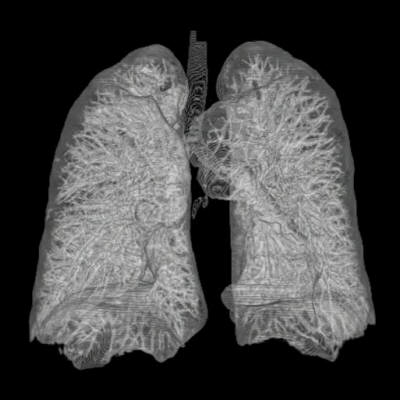
\includegraphics[height=700, alt="Three-dimensional reconstruction of human lungs from CT scans, showing the branching airways"]{Thorax_Lung_3d_from_ct_scans.jpg}
\end{center}
\begin{center}
\small{3d reconstruction of human lungs from CT scans. Andreas Heinemann (CC BY 2.5), Wikimedia}
\end{center}

\slide{Cantor sets}
\begin{columns}[5 6]
For $0<\lambda<1/2$, build $C(\lambda)$ by repeatedly keeping the two outer intervals of relative length $\lambda$ from each interval:
$$C(\lambda)=\bigcap_{k=0}^\infty C_k(\lambda)$$
\begin{itemize}
\item $C_k(\lambda)$ has $2^k$ intervals of length $\lambda^k$
\item the total length of $C_k(\lambda)$ is $(2\lambda)^k\to0$
\end{itemize}
\medskip
Length cannot distinguish $C(1/4)$, $C(1/3)$, $C(9/20)$, but our intuition says that $C(1/4)$ “$<$” $C(1/3)$ “$<$” $C(9/20)$
\columnbreak
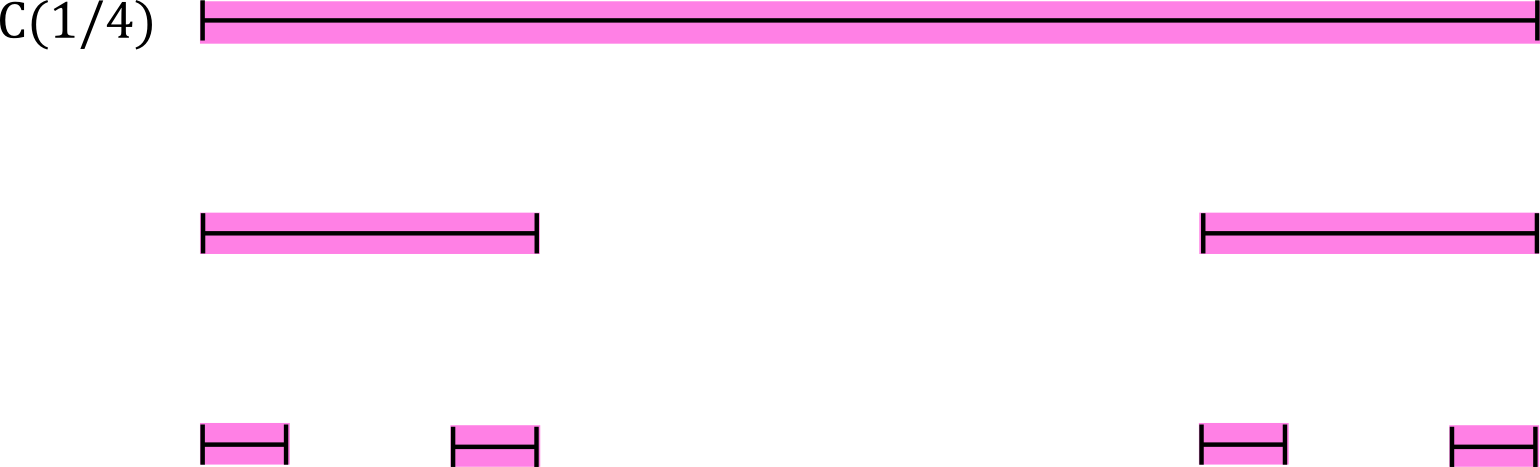
\includegraphics[width=780, alt="The first stages of the Cantor set with lambda = 1/4"]{c1-4.png}
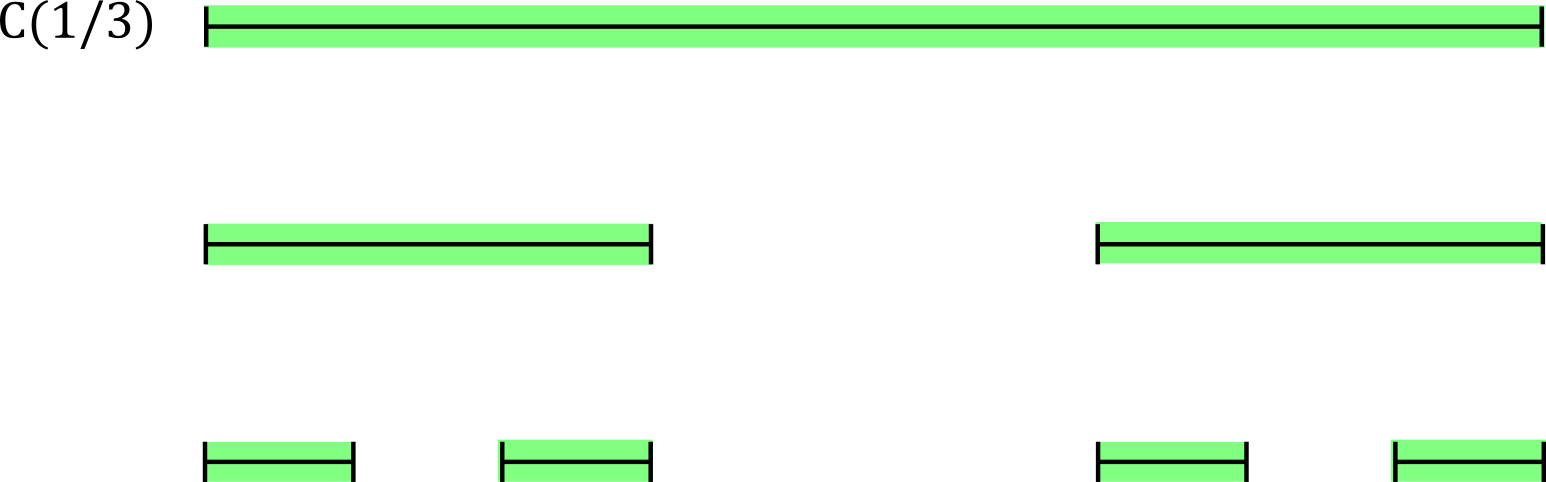
\includegraphics[width=780, alt="The first stages of the Cantor set with lambda = 1/3"]{c1-3.png}
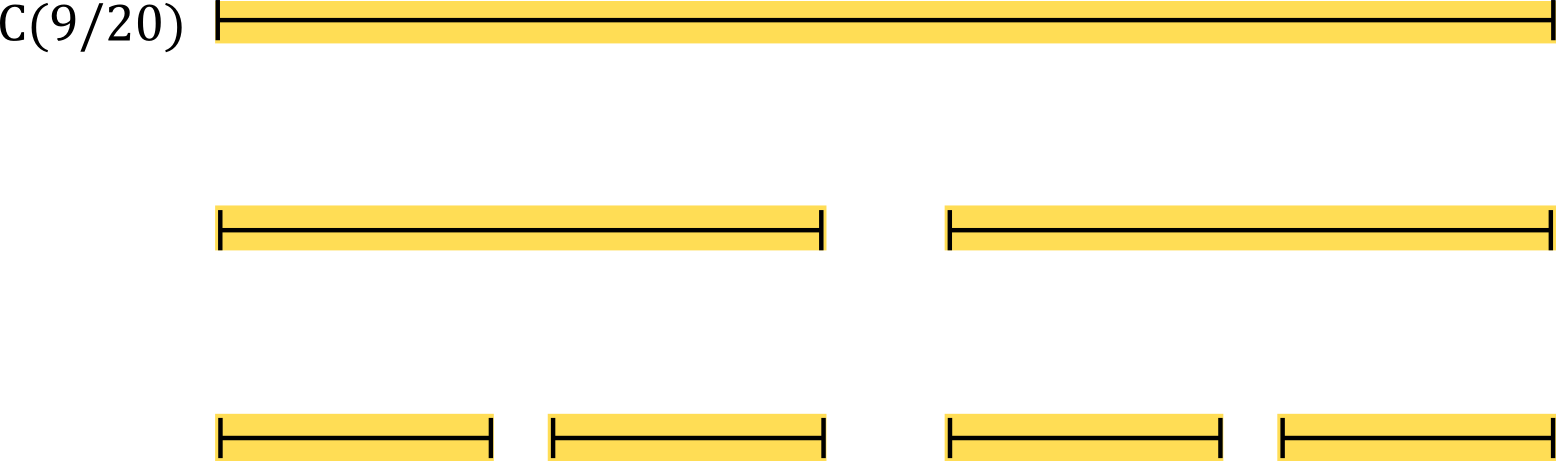
\includegraphics[width=780, alt="The first stages of the Cantor set with lambda = 9/20"]{c9-20.png}
\end{columns}

\slide{Hausdorff content and Hausdorff dimension}
\begin{columns}[7 4]
Cover $A\subseteq\RR^n$ by cubes of any size. A cube of side length $\ell$ costs $\ell^s$. Find the cheapest cover:
$$\textcolor{c1}{\Haus^s_\infty(A)}=\inf\left\{\sum_i(\side Q_i)^s:A\subset\bigcup_iQ_i\right\}$$
$\Haus^s_\infty$ is the (cubical) \textcolor{c1}{\textbf{$s$-dimensional Hausdorff content}}
\medskip
There is a unique $d\in[0,n]$ with $\Haus^s_\infty(A)>0$ for all $s<d$ and $\Haus^s_\infty(A)=0$ for all $s>d$. This number is the \textcolor{c1}{\textbf{Hausdorff dimension}} $\dim_H A$
\columnbreak
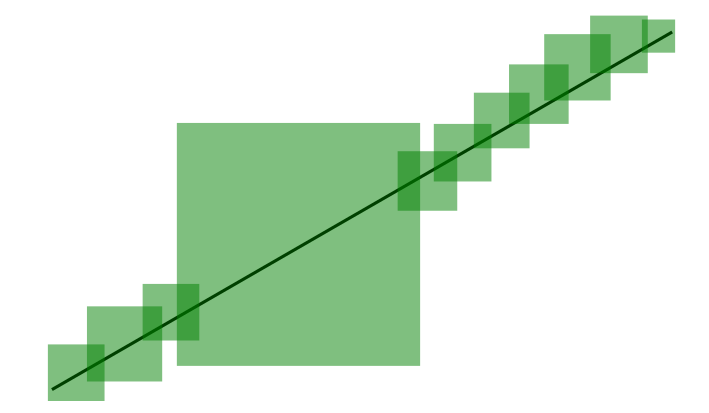
\includegraphics[width=300, alt="A line segment covered by a few cubes of different sizes"]{haus1.png}
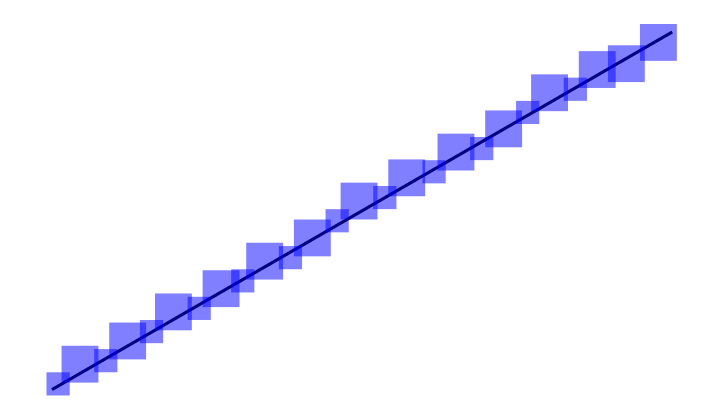
\includegraphics[width=300, alt="A line segment covered by many small cubes"]{haus2.png}
\begin{js}[size=560x340, frames=1, alt="Graph of the Hausdorff content of a set as a function of s: positive and decreasing up to the dimension, then zero up to n"]
const font = (k) => k + "px 'JetBrains Mono', monospace";
const L = 70, B = 70, T = 30, R = 30, X = (s) => L + s / 4.2 * (w - L - R), Y = (v) => h - B - v / 2.3 * (h - B - T);
ctx.strokeStyle = colors.ink; ctx.lineWidth = 3;
ctx.beginPath(); ctx.moveTo(X(0), Y(0)); ctx.lineTo(X(4.2), Y(0)); ctx.moveTo(X(0), Y(0)); ctx.lineTo(X(0), Y(2.3)); ctx.stroke();
ctx.strokeStyle = colors.muted; ctx.setLineDash([8, 8]); ctx.lineWidth = 2; ctx.beginPath(); ctx.moveTo(X(2.2), Y(0)); ctx.lineTo(X(2.2), Y(2.1)); ctx.stroke(); ctx.setLineDash([]);
ctx.strokeStyle = colors.c1; ctx.lineWidth = 7; ctx.beginPath();
for (let k = 0; k <= 40; k++) { const s = 2.2 * k / 40; k ? ctx.lineTo(X(s), Y(1.9 - 0.35 * s)) : ctx.moveTo(X(s), Y(1.9)); }
ctx.stroke(); ctx.beginPath(); ctx.moveTo(X(2.2), Y(0)); ctx.lineTo(X(4), Y(0)); ctx.stroke();
ctx.fillStyle = colors.c1; ctx.beginPath(); ctx.arc(X(2.2), Y(1.9 - 0.77), 7, 0, 2 * Math.PI); ctx.fill();
ctx.fillStyle = colors.ink; ctx.font = font(28); ctx.textAlign = 'center';
ctx.fillText('dim A', X(2.2), Y(0) + 40); ctx.fillText('n', X(4), Y(0) + 40); ctx.fillText('s', X(4.2) - 6, Y(0) - 14);
ctx.fillStyle = colors.c1; ctx.fillText('> 0', X(1.1), Y(1.9) - 6); ctx.fillText('= 0', X(3.1), Y(0) - 18);
\end{js}
\end{columns}
\small{Same null sets and same dimension as the Hausdorff measure $\Haus^s=\lim_{\delta\to0}\Haus^s_\delta$, which only allows cubes of side length at most $\delta$}

\slide{Hausdorff dimension of Cantor sets}
For all $\lambda\in(0,1/2)$, the Cantor set $C(\lambda)$ has Hausdorff dimension
$$\textcolor{c1}{\dim_H C(\lambda)=\frac{\log 2}{\log(1/\lambda)}}\in(0,1)$$
\begin{center}
\textcolor{c1}{Why $\leq$:} covering $C(\lambda)$ by the $2^k$ intervals of $C_k(\lambda)$ costs $2^k\lambda^{ks}=(2\lambda^s)^k$,\\ which tends to $0$ as $k\to\infty$ whenever $2\lambda^s<1$, that is, whenever $s>\log 2/\log(1/\lambda)$
\end{center}
\begin{columns}[1 1 1]
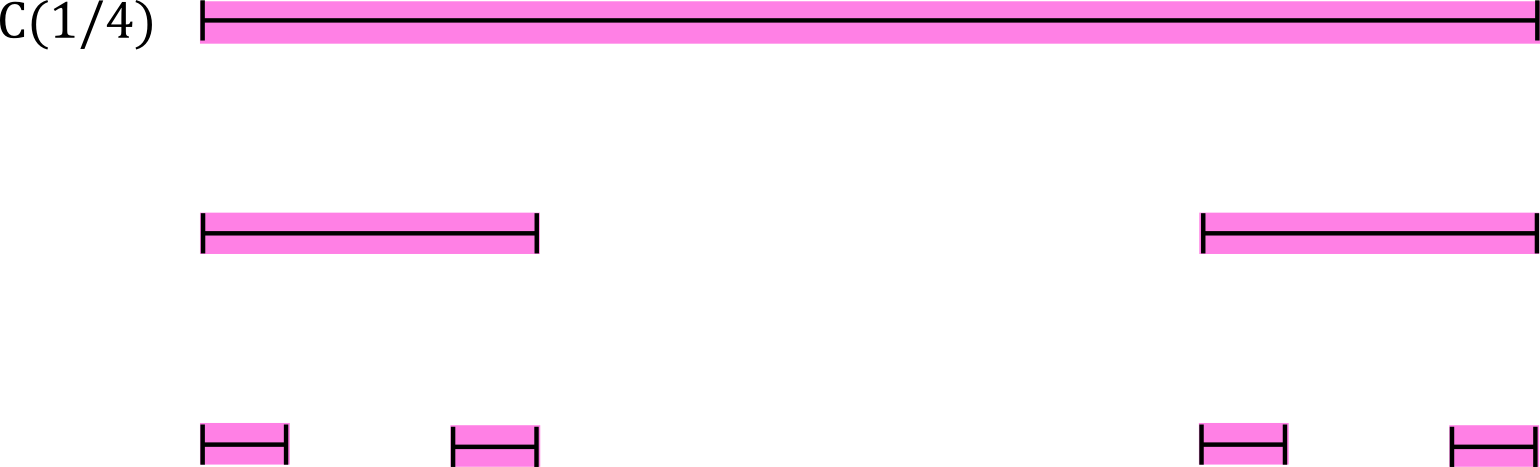
\includegraphics[width=520, alt="Cantor set with lambda = 1/4"]{c1-4.png}
\begin{center}
$\dim_H=0.500\ldots$
\end{center}
\columnbreak
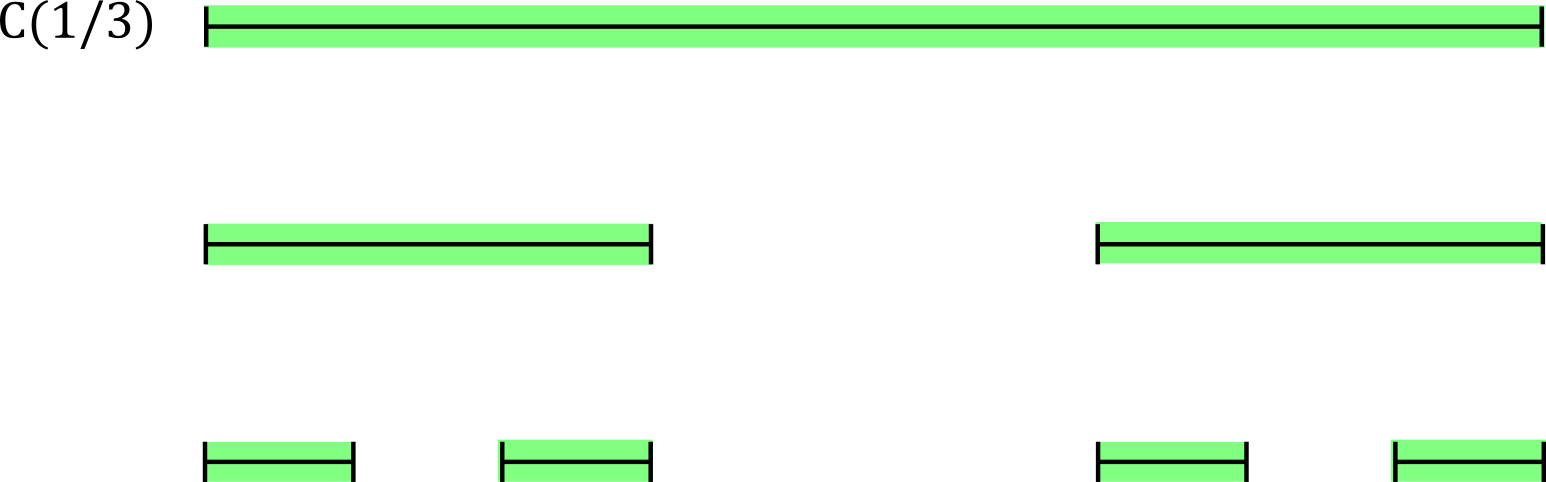
\includegraphics[width=520, alt="Cantor set with lambda = 1/3"]{c1-3.png}
\begin{center}
$\dim_H=0.630\ldots$
\end{center}
\columnbreak
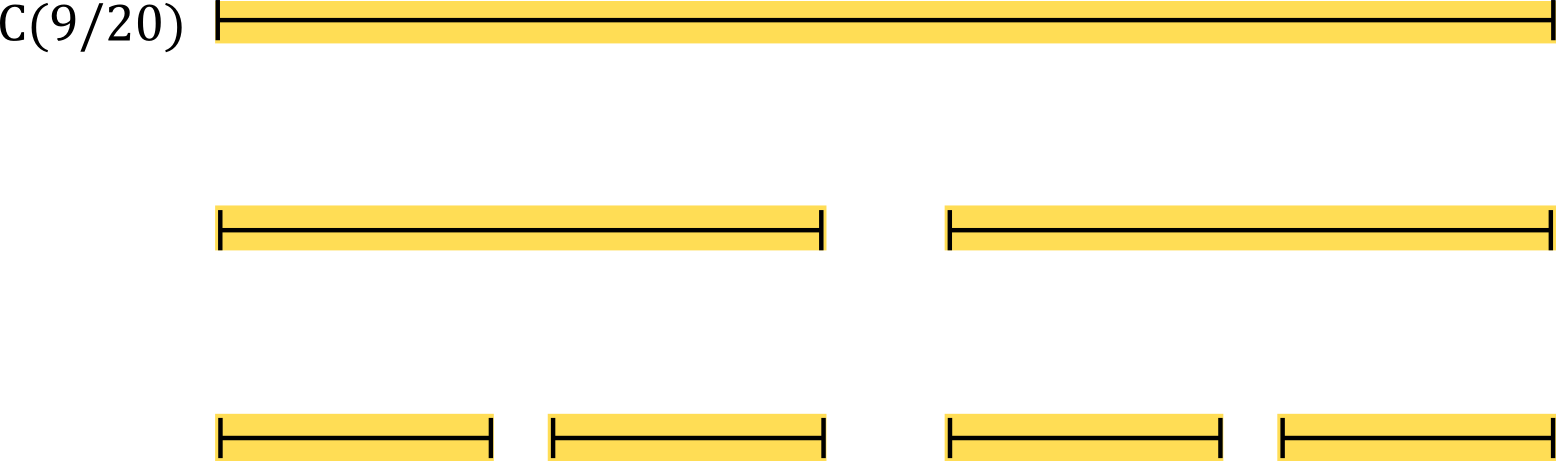
\includegraphics[width=520, alt="Cantor set with lambda = 9/20"]{c9-20.png}
\begin{center}
$\dim_H=0.868\ldots$
\end{center}
\end{columns}

\slide{Dimension of human lungs}
\begin{columns}[9 3]
\heading{Estimates of “fractal dimension” in the literature}
Scaling laws fitted to experimental data on measurements along the branching airways (airway length, airway diameter) lead to:
\columnbreak
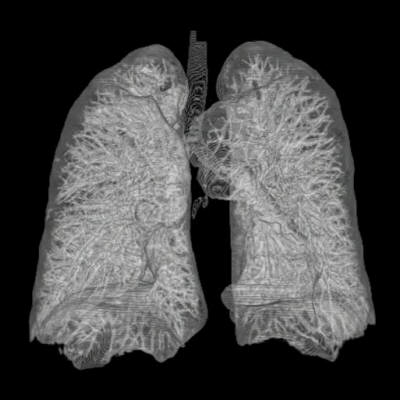
\includegraphics[height=260, alt="Three-dimensional reconstruction of human lungs from CT scans"]{Thorax_Lung_3d_from_ct_scans.jpg}
\end{columns}
\begin{itemize}
\item \accent{\textbf{Nelson and Manchester (1988):}} dimension $\approx2.64$ and $\approx2.76$
\item \accent{\textbf{Nelson, West, and Golden (1990):}} dimension $\approx2.26$ and $\approx2.4$
\item \accent{\textbf{Weibel (1991):}} dimension $\approx2.35$
\item \accent{\textbf{Lamrini Uahabi and Atounti (2017):}} dimension $\approx2.88$
\end{itemize}

\slide{Landing sets for Brownian motion}
\begin{columns}[3 9]
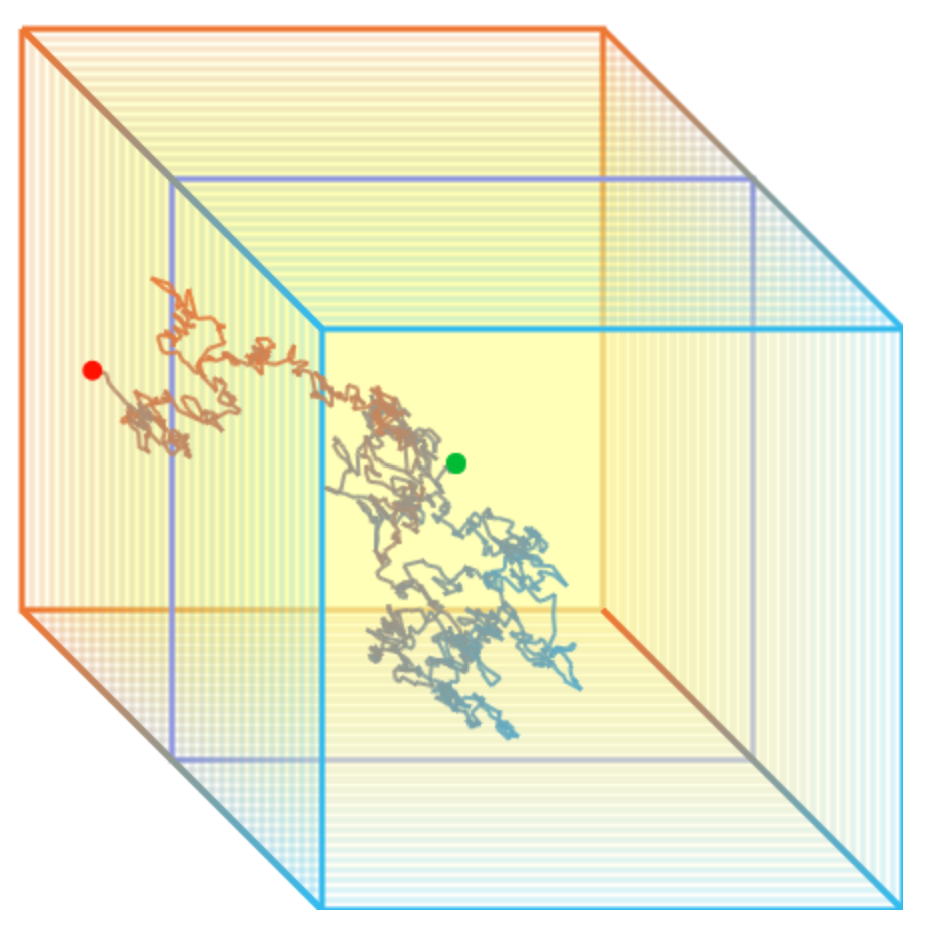
\includegraphics[width=330, alt="Brownian motion in a cube, exiting through a face"]{bm3.png}
\columnbreak
Let $\Omega\subset\RR^n$ be bounded, open, and connected. A set $L\subset\partial\Omega$ is a \textcolor{c3}{\textbf{landing set}} for Brownian motion if almost every path started in $\Omega$ first hits the boundary in $L$: $\;\textcolor{c3}{\omega^X(\partial\Omega\setminus L)=0}$
\medskip
For example, the six \emph{open} faces of the cube $(0,1)^3$, without the edges, form a landing set
\end{columns}
The \textcolor{c3}{\textbf{dimension of harmonic measure on $\Omega$}} is the smallest Hausdorff dimension of a landing set
\medskip
The \textcolor{c3}{\textbf{dimension of harmonic measure on $\RR^n$}} is the largest across all domains:
$$\textcolor{c3}{d_n=\sup_\Omega\udim\,\omega_\Omega},\qquad d_n\geq n-1\quad\text{(take }\Omega=(0,1)^n\text{)}$$

\slide{Dimension drop on the snowflake}
\begin{columns}[4 7]
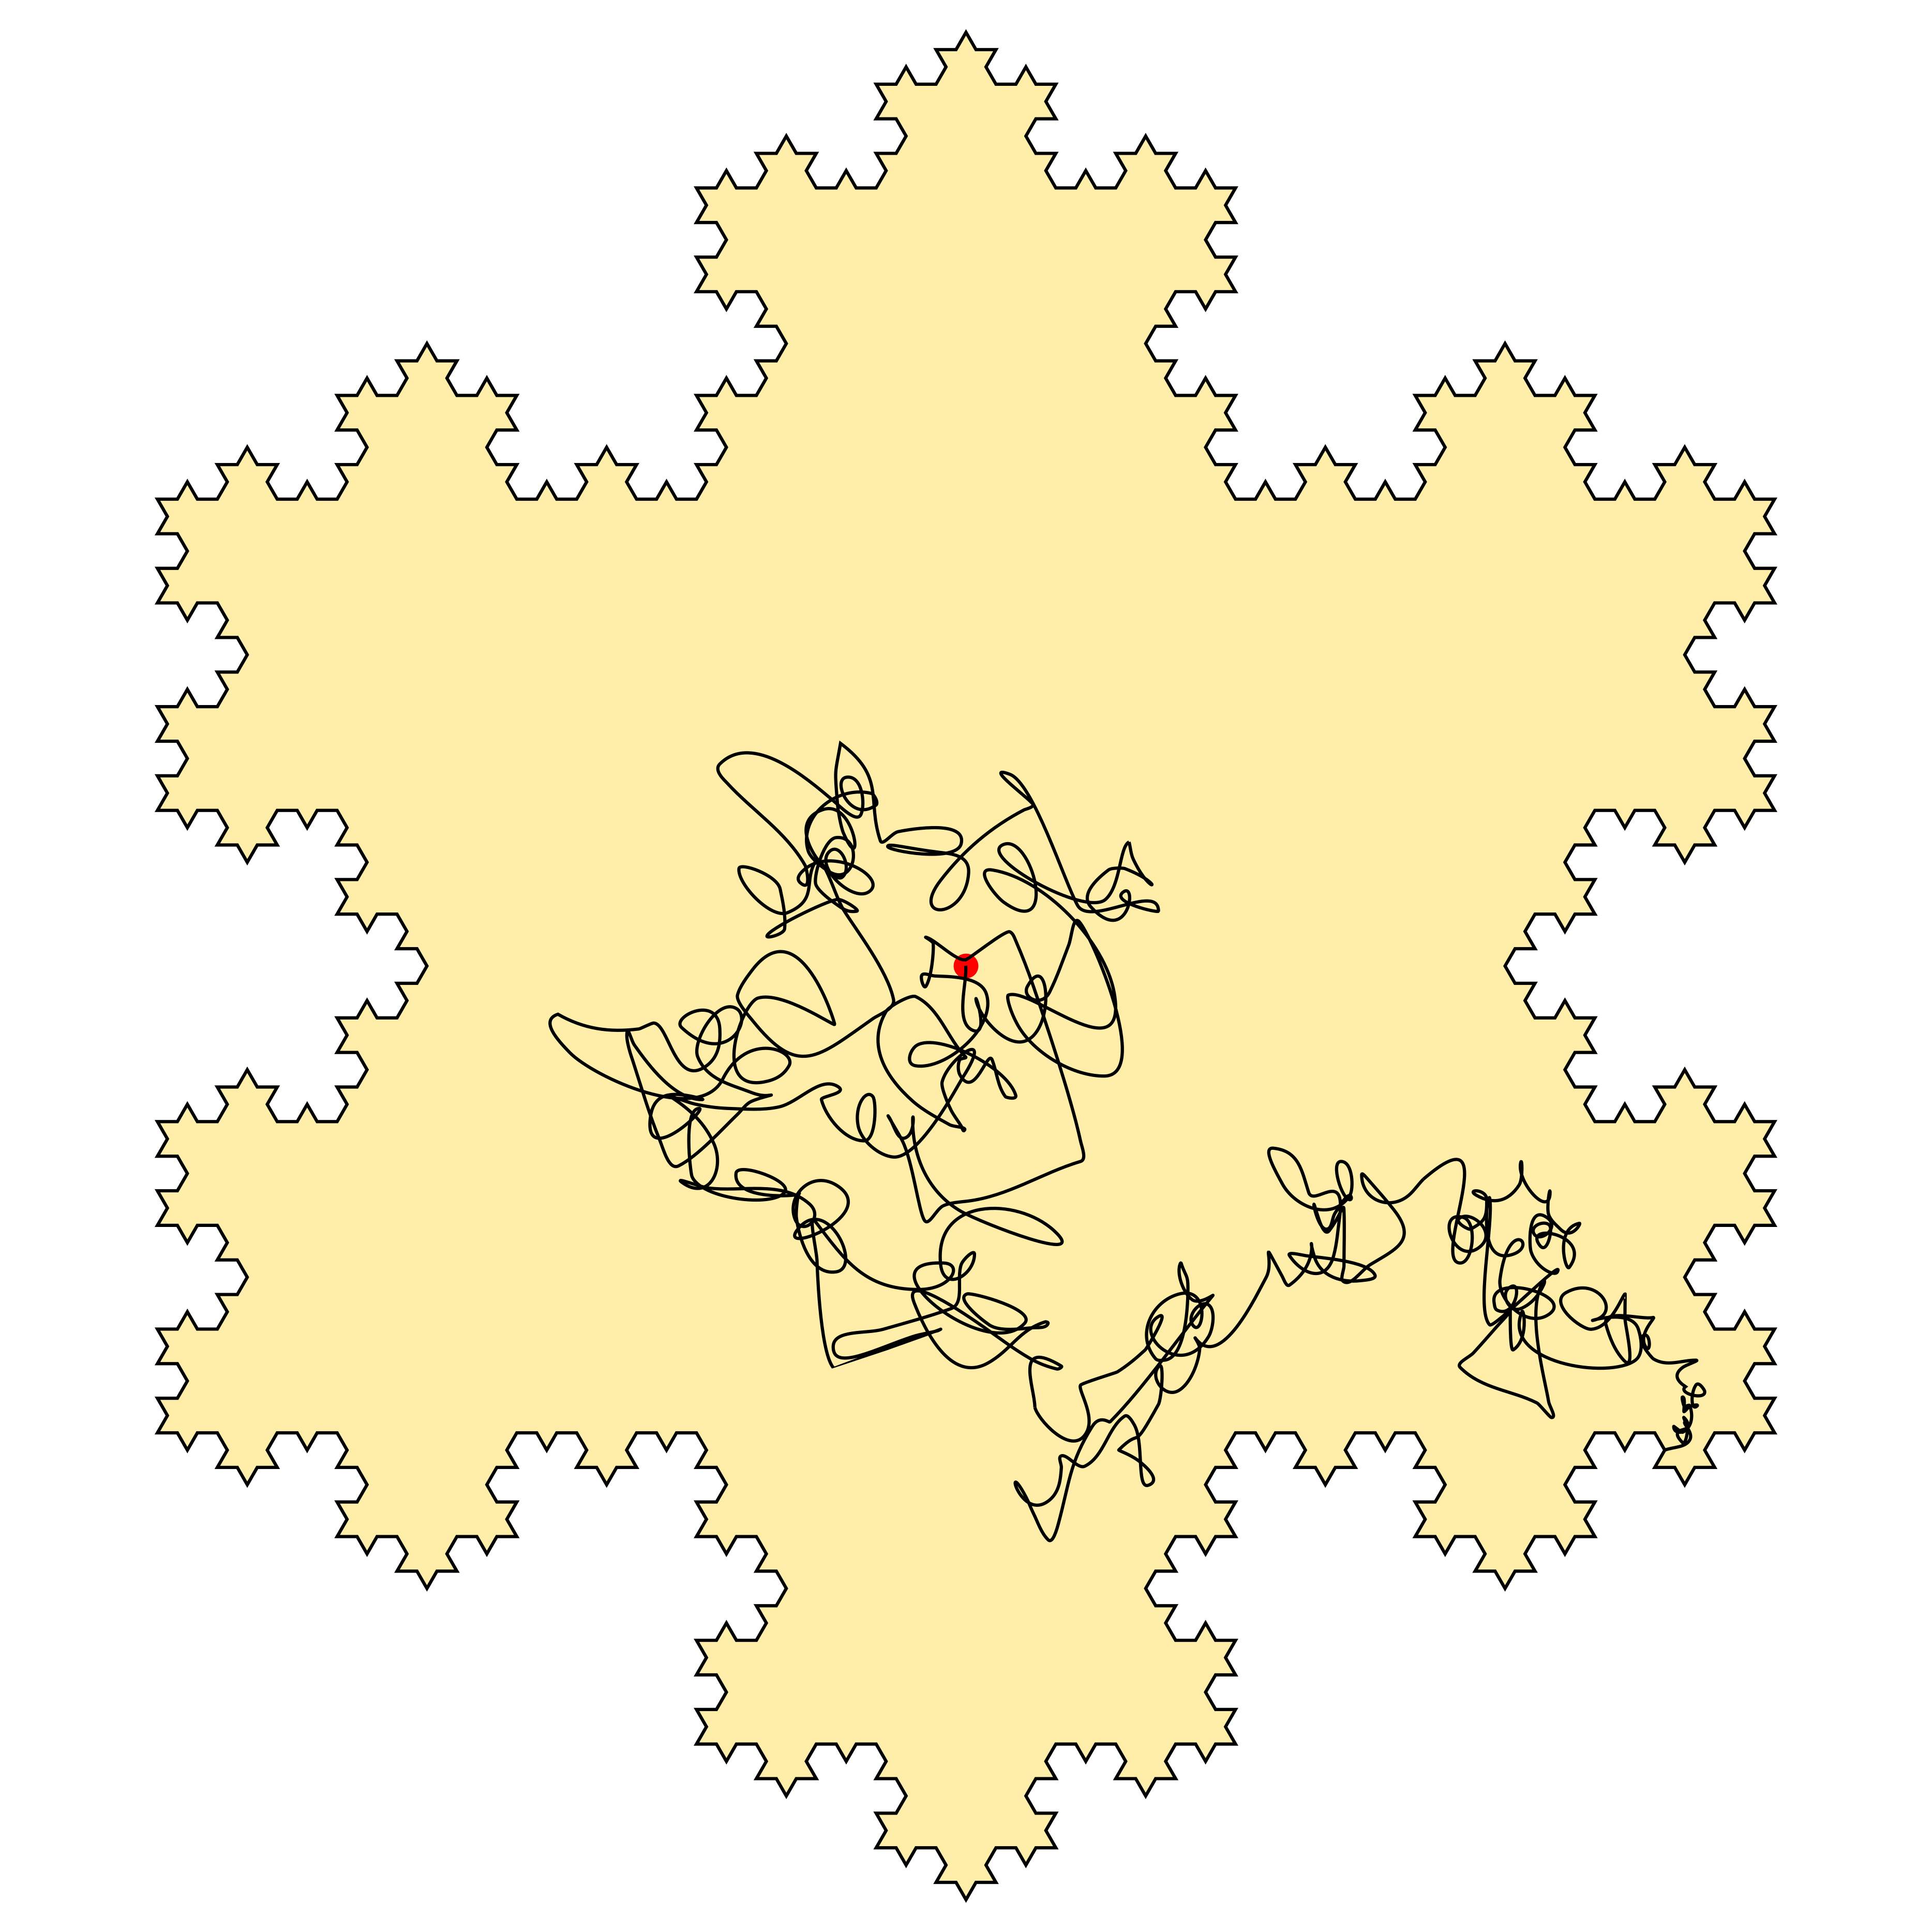
\includegraphics[width=460, alt="The fourth stage of the von Koch snowflake"]{koch4.png}
\begin{center}
$\dim_H\partial\Omega=\log_3 4=1.2618\ldots$
\end{center}
\columnbreak
\heading{Three theorems from 1985}
\begin{itemize}
\item \accent{\textbf{Kaufman and Wu:}} on the snowflake domain, there is a landing set $L$ with $\dim_H L<\dim_H\partial\Omega$. We call this \textcolor{c3}{\textbf{dimension drop}}
\item \accent{\textbf{Carleson:}} on the snowflake domain, there is a landing set $L$ with $\dim_H L=1$
\item \accent{\textbf{Makarov:}} on \emph{every} simply connected planar domain, there is a landing set $L$ with $\dim_H L=1$, and every $E\subset\partial\Omega$ with $\dim_H E<1$ has $\omega_\Omega(E)=0$
\end{itemize}
\end{columns}
\begin{center}
\textcolor{c3}{\textbf{Brownian motion does not see the whole fractal}}
\end{center}

\slide{What do we know about $d_n$?}
Recall $n-1\leq d_n\leq n$
\begin{itemize}
\item \accent{\textbf{Jones and Wolff 1988:}} every planar domain has a landing set of dimension at most 1. Thus, $d_2=1$
\item \accent{\textbf{Wolff 1995:}} there is a domain $\Omega\subset\RR^3$ with $\udim\,\omega_\Omega>2$. Thus, $d_n>n-1$ for all $n\geq3$
\item \accent{\textbf{Bourgain 1987:}} $d_n<n$ for all $n\geq3$. For every domain in $\RR^3$, Brownian motion lands on a set of dimension less than 3
\end{itemize}
\begin{center}
\textcolor{c3}{Back to the lungs: however close to 3 the dimension of the boundary is, Brownian motion lands on a set of dimension at most $d_3<3$}\\ \small{Neither Wolff nor Bourgain says by how much}
\end{center}
\begin{conjecture}{Bishop 1992}
The dimension of harmonic measure in $\RR^n$ is $d_n=n-\frac{1}{n-1}$. In particular, $d_3=2.5$
\end{conjecture}

% ======================================================================
\section*{New results}

\slide[label=results]{What is the dimension of harmonic measure in $\RR^3$?}
\begin{js}[size=1700x360, frames=1, alt="Number line from 2 to 3: Grebenkov et al. numerics at 2.005, Bishop's conjecture at 2.5, and a zoom near 3 showing the new bound 2.99999 and the Badger–Genschaw bound just below 3"]
const font = (k, b) => (b ? '600 ' : '') + k + "px 'JetBrains Mono', monospace";
const L = 60, R = 60, Y0 = 110, X = (v) => L + (v - 2) * (w - L - R);
ctx.fillStyle = '#D9F0D3'; ctx.fillRect(X(2.005), Y0 - 12, X(3) - X(2.005), 24);
ctx.strokeStyle = colors.ink; ctx.lineWidth = 4; ctx.beginPath(); ctx.moveTo(X(2), Y0); ctx.lineTo(X(3), Y0); ctx.stroke();
ctx.font = font(30); ctx.textAlign = 'center'; ctx.fillStyle = colors.ink;
for (const v of [2, 2.5, 3]) { ctx.beginPath(); ctx.moveTo(X(v), Y0 - 18); ctx.lineTo(X(v), Y0 + 18); ctx.stroke(); ctx.fillText(String(v), X(v), Y0 + 56); }
ctx.strokeStyle = colors.c4; ctx.lineWidth = 6; ctx.beginPath(); ctx.moveTo(X(2.005), Y0 - 30); ctx.lineTo(X(2.005), Y0 + 30); ctx.stroke();
ctx.fillStyle = colors.c4; ctx.textAlign = 'left'; ctx.font = font(26); ctx.fillText('Grebenkov et al. numerics: ≥ 2.005', X(2.005) - 4, Y0 - 44);
ctx.fillStyle = colors.c1; ctx.beginPath(); ctx.arc(X(2.5), Y0, 12, 0, 2 * Math.PI); ctx.fill();
ctx.textAlign = 'center'; ctx.fillText("Bishop's conjecture: 2.5", X(2.5), Y0 - 34);
// zoom near 3
const ZX0 = 980, ZX1 = w - R, ZY = 280, Z = (v) => ZX0 + (v - 2.99998) / 0.00002 * (ZX1 - ZX0);
ctx.strokeStyle = colors.muted; ctx.lineWidth = 2;
ctx.strokeRect(X(2.988), Y0 - 26, X(3) - X(2.988) + 8, 52);
ctx.beginPath(); ctx.moveTo(X(2.988), Y0 + 26); ctx.lineTo(ZX0 - 20, ZY - 50); ctx.moveTo(X(3) + 8, Y0 + 26); ctx.lineTo(ZX1 + 20, ZY - 50); ctx.stroke();
ctx.fillStyle = '#D9F0D3'; ctx.fillRect(ZX0, ZY - 10, Z(2.99999) - ZX0, 20);
ctx.strokeStyle = colors.ink; ctx.lineWidth = 3; ctx.beginPath(); ctx.moveTo(ZX0, ZY); ctx.lineTo(ZX1, ZY); ctx.stroke();
ctx.fillStyle = colors.ink; ctx.font = font(24);
for (const [v, t] of [[2.99998, '2.99998'], [3, '3']]) { ctx.beginPath(); ctx.moveTo(Z(v), ZY - 12); ctx.lineTo(Z(v), ZY + 12); ctx.stroke(); ctx.fillText(t, Z(v), ZY + 44); }
ctx.strokeStyle = colors.c4; ctx.lineWidth = 6; ctx.beginPath(); ctx.moveTo(Z(2.99999), ZY - 28); ctx.lineTo(Z(2.99999), ZY + 28); ctx.stroke();
ctx.fillStyle = colors.c4; ctx.font = font(26, true); ctx.fillText('2.99999 (new)', Z(2.99999), ZY - 40);
ctx.strokeStyle = colors.c3; ctx.beginPath(); ctx.moveTo(Z(3) - 4, ZY - 28); ctx.lineTo(Z(3) - 4, ZY); ctx.stroke();
ctx.fillStyle = colors.c3; ctx.font = font(24); ctx.textAlign = 'right'; ctx.fillText('B–G 2024', Z(3) - 10, ZY - 40);
\end{js}
\begin{columns}[1 1]
\begin{theorem}{Badger–Genschaw 2024}
$d_3<2.99999\,99999\,99999$
\medskip
$d_n<n-\left(\frac{1}{n-1}\right)^{2n^2}$ for all $n\gg3$
\end{theorem}
\columnbreak
\begin{theorem}{new bound, 2026}
$\alert{d_3<2.99999}$
\medskip
$\textcolor{c4}{d_n<n-\left(\frac{1}{n-1}\right)^{2n+6.12\sqrt n}}$ for all $n\geq3$
\end{theorem}
\end{columns}
\begin{center}
On the scale $n-d_n\approx(n-1)^{-E}$, the exponent improves from $E=2n^2$ to $\textcolor{c4}{E=2n+O(\sqrt n)}$\\ Bishop's conjecture is $E=1$ \goto{app-params}{parameters}
\end{center}

\slide[label=strategy]{Bourgain's strategy: a dichotomy at every scale}
Fix $s=n-\rho$ slightly less than $n$. Look at the boundary $\partial\Omega$ inside each cube $P$
\begin{columns}[1 1]
\heading{\textcolor{c1}{Alternative I: there is a hole}}
Then smaller cubes $Q_i$ cover $\partial\Omega\cap P$ efficiently: $\textcolor{c1}{\sum_i(\side Q_i)^s\leq(\side P)^s}$
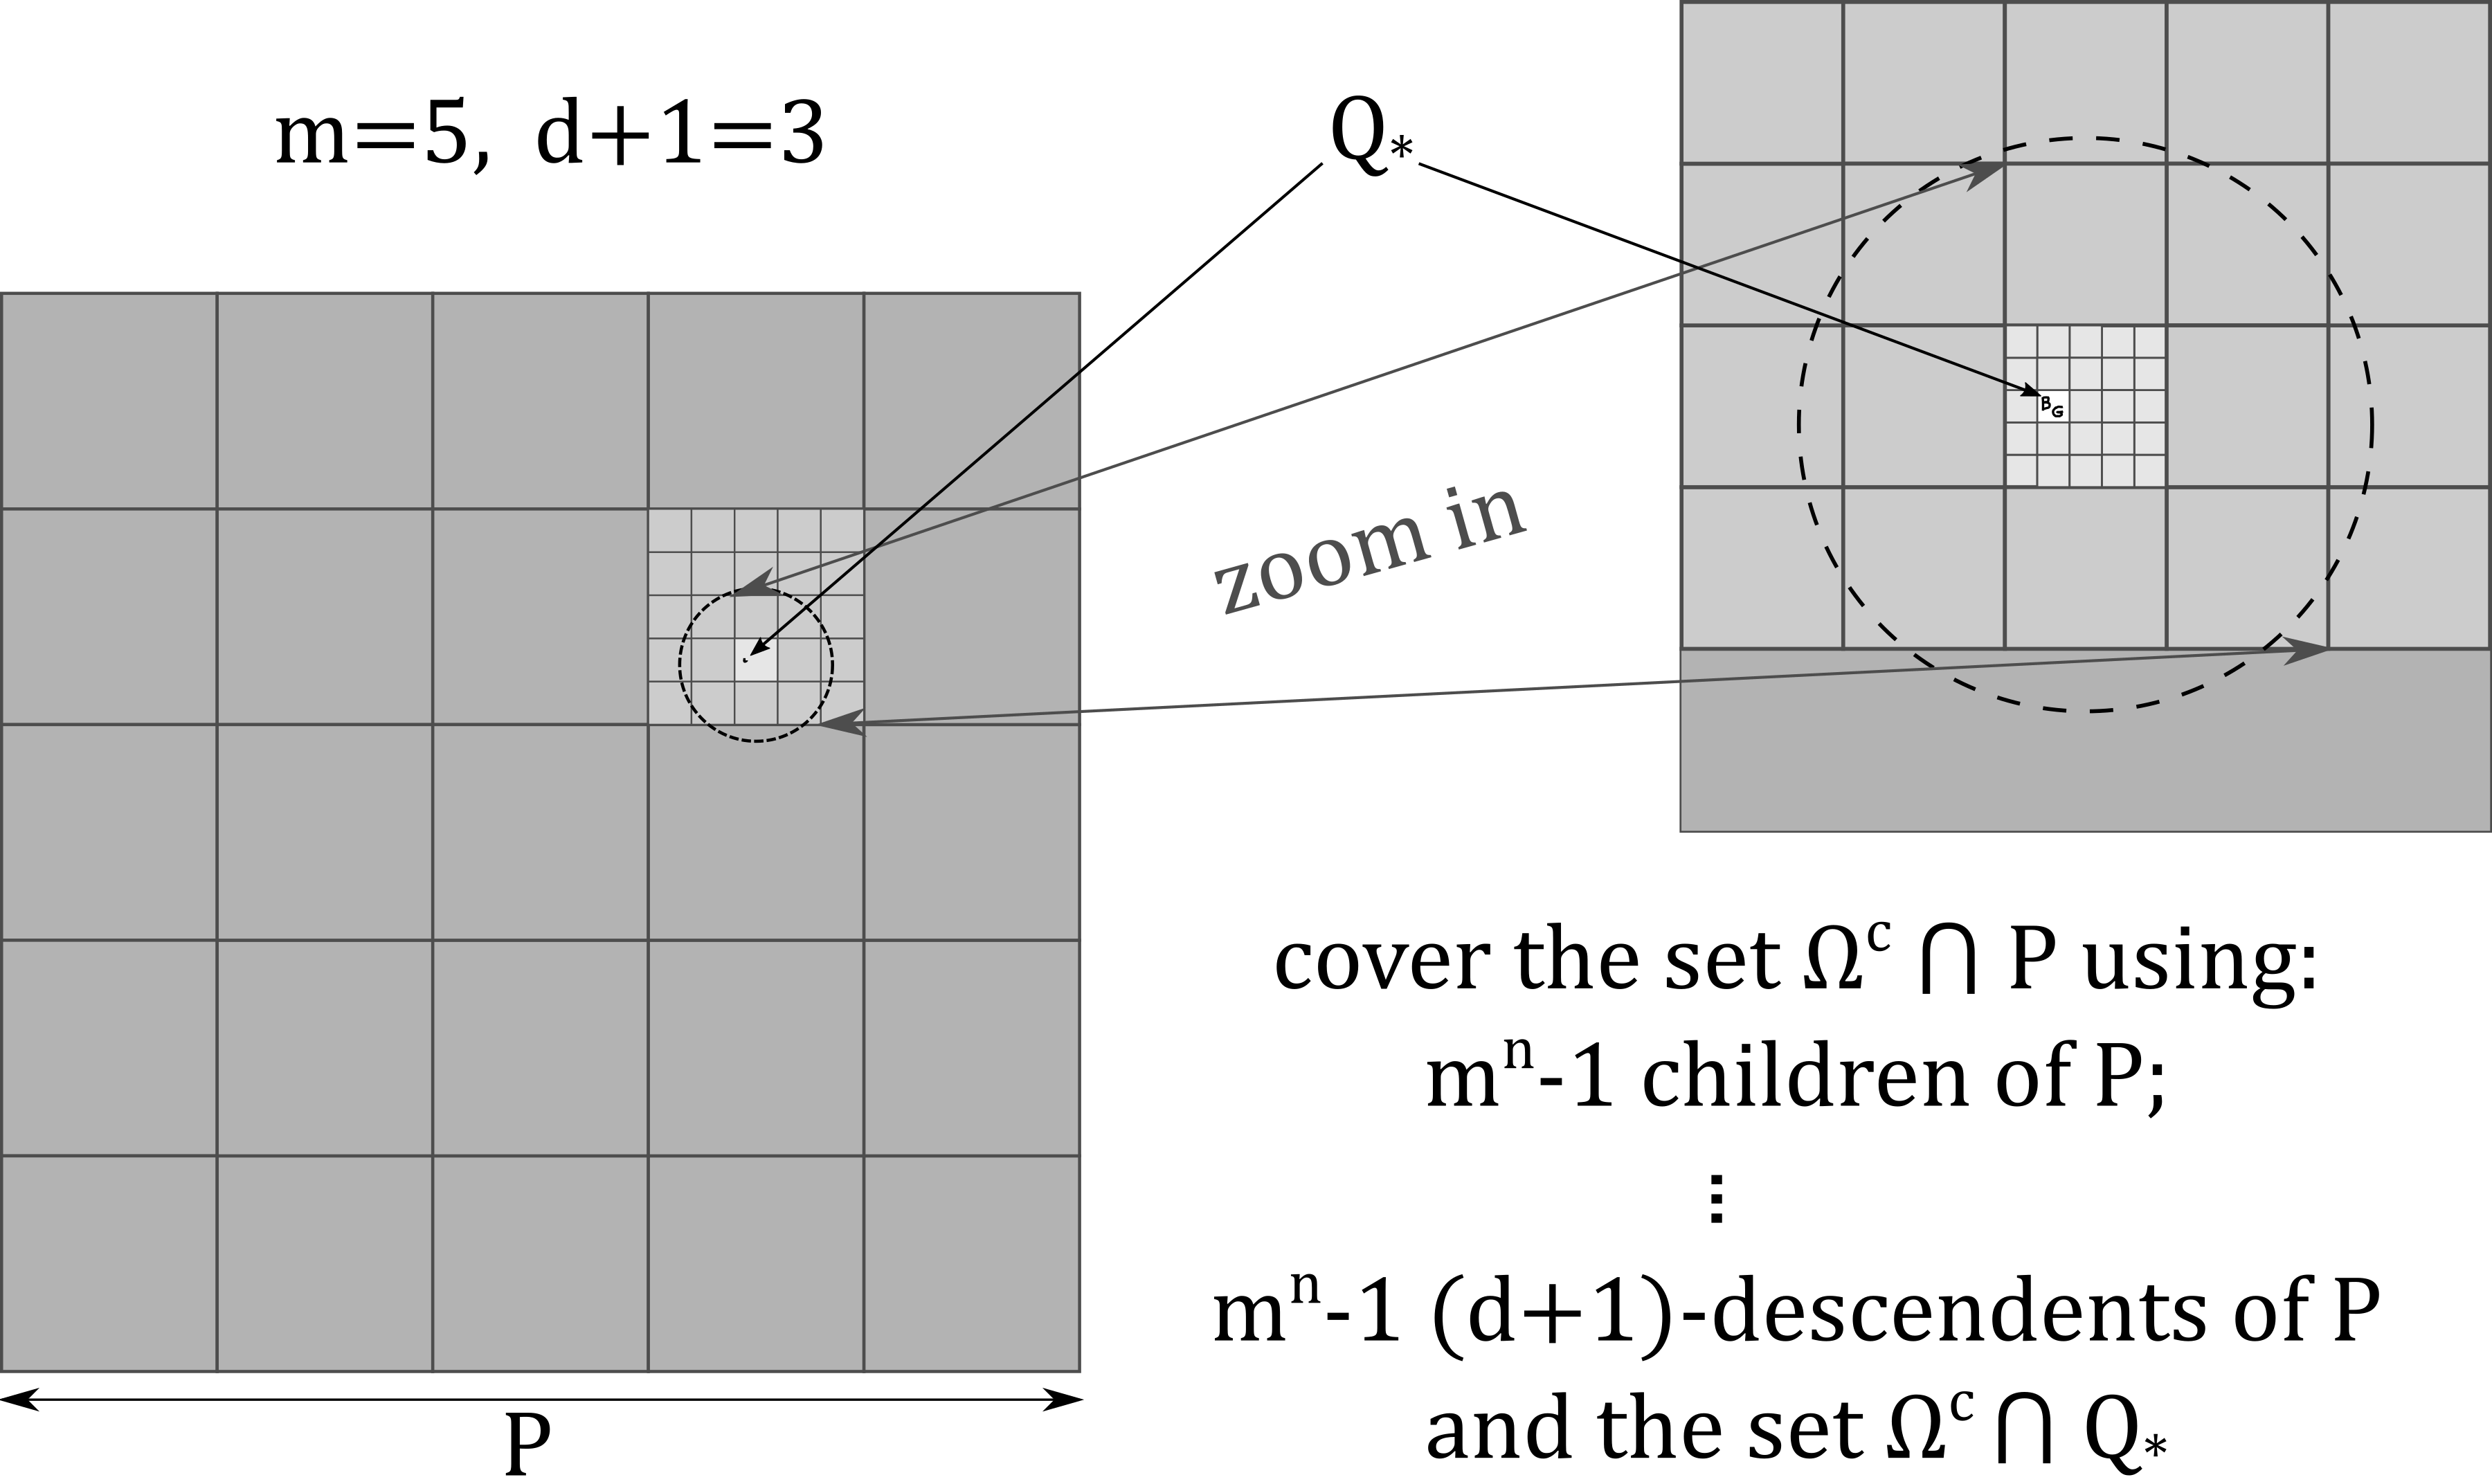
\includegraphics[height=300, alt="A hole in the boundary inside a cube, seen by zooming in"]{alt1.png}
\columnbreak
\heading{\textcolor{c3}{Alternative II: there is no hole}}
Then $\partial\Omega$ is a \textcolor{c3}{barrier}: Brownian motion rarely reaches deep inside $P$, which a constant $\lambda$ quantifies
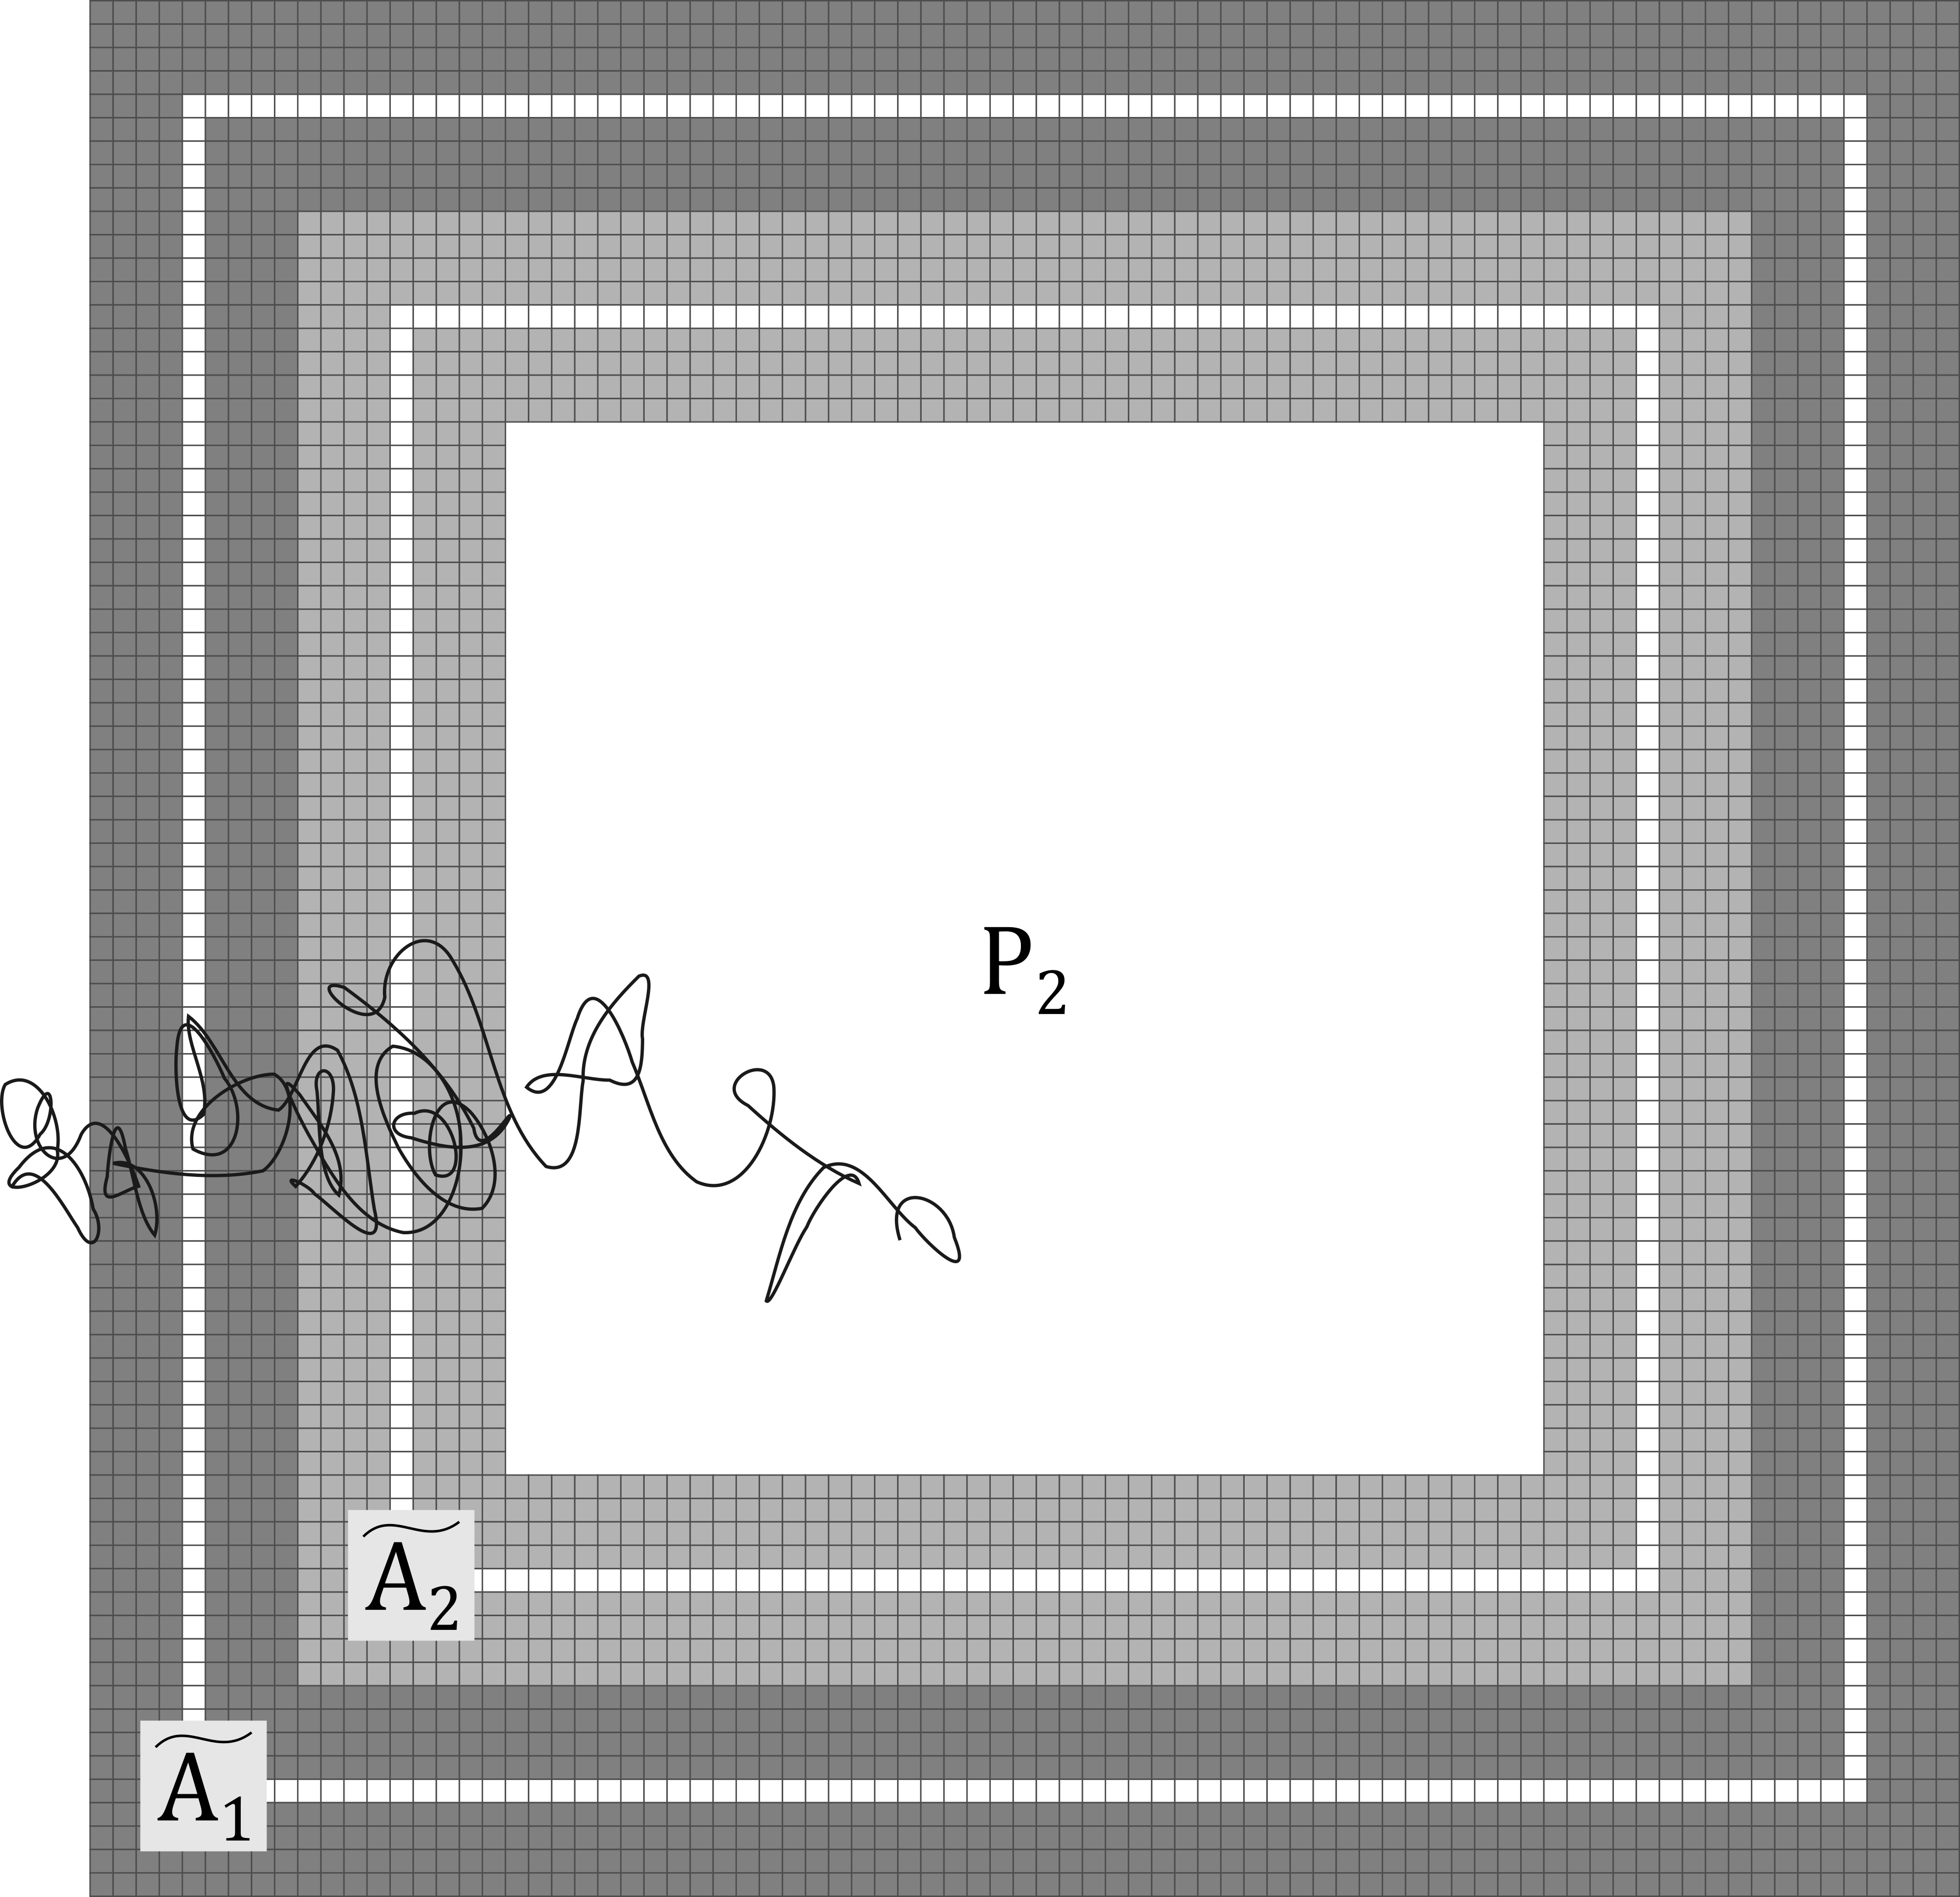
\includegraphics[height=300, alt="Concentric rings of cubes with no holes, and a Brownian path stopped near the outer ring"]{alt2.png}
\end{columns}
\begin{center}
If one of the alternatives holds for every cube, then $\alert{\udim\,\omega_\Omega\leq n-\lambda\rho/(1+\lambda)}$\\ \small{Pictures: the model of Badger–Genschaw with a fixed $m$-adic grid} \goto{app-dimlemma}{dimension lemma} \goto{app-altI}{Alternative I}
\end{center}
\slide{Simulation: a dust of cubes as a barrier}
\begin{js}[size=1640x680, frames=1, alt="Interactive: a random dust of small cubes in a spherical shell, drawn in three dimensions and rotating; Brownian paths start at the center and stop when they hit the dust (purple, with a mark where they land) or when they reach a sphere of radius 3 (gray); a slider sets the density of the dust; drag to rotate"]
const font = (k, b) => (b ? '600 ' : '') + k + "px 'JetBrains Mono', monospace";
const CX = 350, CY = 345, U = 3, SC = 300, LW = 720;
const TX0 = 780, TX1 = 1580, PY0 = 110, P0 = 0.25, P1 = 0.65, DEPTH = 6, TOP = 5, HALF = 1, EPS = 1e-3, S = 2.99993;
const trunc = (v, d) => { const f = Math.pow(10, d); return (Math.floor(v * f + 1e-12) / f).toFixed(d) + '…'; };
canvas.style.touchAction = 'none';
if (state.p === undefined) { state.p = 0.45; state.yaw = 0.5; state.pitch = 0.35; state.auto = true; }
function hash(a, b, c, d) { let h = 2166136261 ^ a; h = Math.imul(h ^ b, 16777619); h = Math.imul(h ^ c, 16777619); h = Math.imul(h ^ d, 16777619); h ^= h >>> 13; h = Math.imul(h, 0x5bd1e995); h ^= h >>> 15; return (h >>> 0) / 4294967296; }
function build() {
  const leaves = [];
  // dyadic dust in the unit ball, kept in the shell 0.5 < |x| < 0.9; a cube survives with probability p at each level,
  // and the same random numbers are used for every p, so the dust grows with p
  function rec(ix, iy, iz, lev) {
    const e = 2 * HALF / Math.pow(2, lev), x = -HALF + ix * e, y = -HALF + iy * e, z = -HALF + iz * e;
    if (lev === DEPTH) {
      const r = Math.hypot(x + e / 2, y + e / 2, z + e / 2);
      if (r > 0.5 && r < 0.9) { leaves.push([ix, iy, iz]); return { x: x, y: y, z: z, e: e, lev: lev, leaf: true }; }
      return null;
    }
    const kids = [];
    for (let c = 0; c < 8; c++) {
      const jx = 2 * ix + (c & 1), jy = 2 * iy + (c >> 1 & 1), jz = 2 * iz + (c >> 2 & 1);
      if (hash(lev + 1, jx, jy, jz) < state.p) { const k = rec(jx, jy, jz, lev + 1); if (k) kids.push(k); }
    }
    return kids.length ? { x: x, y: y, z: z, e: e, lev: lev, kids: kids } : null;
  }
  state.tree = rec(0, 0, 0, 0);
  // the faces of the dust that are not shared by two of its cubes
  const E = 2 * HALF / Math.pow(2, DEPTH), key = (a, b, c) => (a * 64 + b) * 64 + c, has = new Set(leaves.map((l) => key(l[0], l[1], l[2])));
  const faces = [];
  for (const [ix, iy, iz] of leaves) for (let ax = 0; ax < 3; ax++) for (const sg of [-1, 1]) {
    const nb = [ix, iy, iz]; nb[ax] += sg;
    if (has.has(key(nb[0], nb[1], nb[2]))) continue;
    const lo = [-HALF + ix * E, -HALF + iy * E, -HALF + iz * E], b = (ax + 1) % 3, c = (ax + 2) % 3;
    const q = (db, dc) => { const v = lo.slice(); if (sg > 0) v[ax] += E; v[b] += db * E; v[c] += dc * E; return v; };
    const n = [0, 0, 0]; n[ax] = sg;
    faces.push({ P: [q(0, 0), q(1, 0), q(1, 1), q(0, 1)], n: n, c: [lo[0] + E / 2 + n[0] * E / 2, lo[1] + E / 2 + n[1] * E / 2, lo[2] + E / 2 + n[2] * E / 2] });
  }
  state.faces = faces; state.cubes = leaves.length;
  // net content: a dyadic net with initial scale 2r/h, r = 1, h = 32 (cubes of side 1/16 and smaller)
  function cont(nd) {
    if (!nd) return 0;
    if (nd.leaf) return Math.pow(nd.e, S);
    let t = 0; for (const k of nd.kids) t += cont(k);
    return nd.lev >= TOP ? Math.min(Math.pow(nd.e, S), t) : t;
  }
  state.content = cont(state.tree);
  // Bourgain's estimate with n = 3, g = 2, r = 1
  state.bound = (2 / 3) * (1 - 0.5) / (1 + Math.pow(3, -6)) * state.content / (4 * Math.PI / 3);
  state.walks = 0; state.hits = 0; state.paths = []; state.marks = []; state.cache = null;
}
function dbox(px, py, pz, nd) {
  const dx = Math.max(nd.x - px, 0, px - nd.x - nd.e), dy = Math.max(nd.y - py, 0, py - nd.y - nd.e), dz = Math.max(nd.z - pz, 0, pz - nd.z - nd.e);
  return Math.hypot(dx, dy, dz);
}
function distE(px, py, pz) {
  let best = Infinity;
  (function rec(nd) { if (!nd) return; const d = dbox(px, py, pz, nd); if (d >= best) return; if (nd.leaf) { best = d; return; } for (const k of nd.kids) rec(k); })(state.tree);
  return best;
}
let spare = null;
function gauss() {                                          // standard normal (Box–Muller)
  if (spare !== null) { const g = spare; spare = null; return g; }
  const u = 1 - Math.random(), v = Math.random(), r = Math.sqrt(-2 * Math.log(u));
  spare = r * Math.sin(2 * Math.PI * v); return r * Math.cos(2 * Math.PI * v);
}
// Brownian motion sampled at times adapted to the distance d to the boundary: each increment is exactly
// N(0, (C d)^2 I), so the sampled points lie on a true Brownian path; with C = 0.2 the chance that the path
// leaves and re-enters between two samples is negligible, and the walk stops within EPS of the boundary
const C = 0.2;
function walk() {
  let x = 0, y = 0, z = 0; const path = [[0, 0, 0]];
  for (let i = 0; i < 200000; i++) {
    const dE = distE(x, y, z), dU = U - Math.hypot(x, y, z), d = Math.min(dE, dU);
    if (dE < EPS) return { path: path, hit: true, end: [x, y, z] };
    if (dU < EPS) return { path: path, hit: false };
    const sd = C * d; x += sd * gauss(); y += sd * gauss(); z += sd * gauss(); path.push([x, y, z]);
  }
  return { path: path, hit: false };
}
// perspective view: turn by yaw about the vertical axis, then tilt by pitch
function view(p) {
  const cy = Math.cos(state.yaw), sy = Math.sin(state.yaw), cp = Math.cos(state.pitch), sp = Math.sin(state.pitch);
  const x1 = p[0] * cy - p[1] * sy, y1 = p[0] * sy + p[1] * cy;
  const depth = y1 * cp - p[2] * sp, up = y1 * sp + p[2] * cp, f = 5 / (5 + depth);
  return [CX + SC * f * x1, CY - SC * f * up, depth];
}
function viewDir(n) {
  const cy = Math.cos(state.yaw), sy = Math.sin(state.yaw), cp = Math.cos(state.pitch), sp = Math.sin(state.pitch);
  const x1 = n[0] * cy - n[1] * sy, y1 = n[0] * sy + n[1] * cy;
  return [x1, y1 * cp - n[2] * sp, y1 * sp + n[2] * cp];
}
// the dust is drawn into two layers, the half behind the center and the half in front of it,
// and redrawn only when the view or the dust changes
function layers() {
  const key = state.yaw.toFixed(3) + ',' + state.pitch.toFixed(3);
  if (state.cache && state.cache.key === key) return state.cache;
  const mk = () => { const c = document.createElement('canvas'); c.width = LW; c.height = h; return c; };
  const back = state.cache ? state.cache.back : mk(), front = state.cache ? state.cache.front : mk();
  const bx = back.getContext('2d'), fx = front.getContext('2d');
  bx.clearRect(0, 0, LW, h); fx.clearRect(0, 0, LW, h);
  const vis = [];
  for (const F of state.faces) {
    const d = viewDir(F.n); if (d[1] >= 0) continue;           // the face points away from the viewer
    const P = F.P.map(view), cd = view(F.c)[2];
    // light from the upper left, in front of the viewer
    const lit = Math.max(0, -0.45 * d[0] + 0.55 * d[2] - 0.7 * d[1]);
    vis.push([P, cd, 0.45 + 0.55 * lit, view([F.c[0], F.c[1], F.c[2]])[2] > 0]);
  }
  vis.sort((a, b) => b[1] - a[1]);
  for (const [P, , L, far] of vis) {
    const g = far ? bx : fx, k = (v) => Math.round(v * L);
    g.fillStyle = 'rgb(' + k(70) + ',' + k(118) + ',' + k(214) + ')'; g.strokeStyle = 'rgba(20,30,60,0.35)'; g.lineWidth = 0.8;
    g.beginPath(); P.forEach((q, i) => i ? g.lineTo(q[0], q[1]) : g.moveTo(q[0], q[1])); g.closePath(); g.fill(); g.stroke();
  }
  state.cache = { key: key, back: back, front: front };
  return state.cache;
}
function draw() {
  ctx.clearRect(0, 0, w, h);
  const L = layers();
  ctx.save(); ctx.beginPath(); ctx.rect(0, 0, LW, h); ctx.clip();
  // the unit ball
  ctx.strokeStyle = colors.muted; ctx.lineWidth = 2; ctx.setLineDash([10, 8]);
  ctx.beginPath(); ctx.arc(CX, CY, SC, 0, 2 * Math.PI); ctx.stroke(); ctx.setLineDash([]);
  ctx.drawImage(L.back, 0, 0);
  for (const p of state.paths) {
    ctx.strokeStyle = p.hit ? 'rgba(142,58,138,0.75)' : 'rgba(120,120,120,0.4)'; ctx.lineWidth = 1.6;
    // only the part of each path near the unit ball is drawn
    ctx.beginPath(); let inside = false;
    for (const q of p.path) { const v = view(q), ok = Math.hypot(q[0], q[1], q[2]) < 1.15; if (ok && inside) ctx.lineTo(v[0], v[1]); else ctx.moveTo(v[0], v[1]); inside = ok; }
    ctx.stroke();
  }
  ctx.fillStyle = 'rgba(142,58,138,0.55)';
  for (const m of state.marks) { const v = view(m); ctx.beginPath(); ctx.arc(v[0], v[1], 2.2, 0, 2 * Math.PI); ctx.fill(); }
  ctx.fillStyle = colors.alert; ctx.beginPath(); const o = view([0, 0, 0]); ctx.arc(o[0], o[1], 8, 0, 2 * Math.PI); ctx.fill();
  ctx.globalAlpha = 0.45; ctx.drawImage(L.front, 0, 0); ctx.globalAlpha = 1;
  ctx.restore();
  // panel
  ctx.fillStyle = colors.ink; ctx.font = font(34); ctx.textAlign = 'left'; ctx.fillText('density of the dust p = ' + state.p.toFixed(2), TX0, PY0 - 34);
  ctx.strokeStyle = colors.grid; ctx.lineWidth = 10; ctx.lineCap = 'round'; ctx.beginPath(); ctx.moveTo(TX0, PY0); ctx.lineTo(TX1, PY0); ctx.stroke();
  const sx = TX0 + (state.p - P0) / (P1 - P0) * (TX1 - TX0);
  ctx.strokeStyle = colors.c1; ctx.beginPath(); ctx.moveTo(TX0, PY0); ctx.lineTo(sx, PY0); ctx.stroke();
  ctx.fillStyle = colors.c1; ctx.beginPath(); ctx.arc(sx, PY0, 17, 0, 2 * Math.PI); ctx.fill();
  const n = state.walks, f = n ? state.hits / n : 0, se = n ? Math.sqrt(f * (1 - f) / n) : 0;
  const rows = [
    ['content of the dust (dyadic cubes)', trunc(state.content, 4), colors.c1],
    ['Bourgain’s lower bound', trunc(state.bound, 4), colors.c1],
    ['fraction of ' + n + ' paths that hit the dust', n ? f.toFixed(3) + ' ± ' + (2 * se).toFixed(3) : '…', colors.c3]
  ];
  let y = 230;
  for (const row of rows) {
    ctx.fillStyle = colors.text; ctx.textAlign = 'left'; ctx.font = font(30); ctx.fillText(row[0], TX0, y);
    ctx.fillStyle = row[2]; ctx.font = font(38, true); ctx.fillText(row[1], TX0, y + 48); y += 125;
  }
  ctx.fillStyle = colors.muted; ctx.font = font(24);
  ctx.fillText(state.cubes + ' cubes of side 1/32 in the shell 0.5 < |x| < 0.9', TX0, 600);
  ctx.fillText('paths stop on the dust or at radius 3', TX0, 636); ctx.fillText('purple dots: where paths land; drag to rotate', TX0, 670);
}
function pos(e) { const b = canvas.getBoundingClientRect(); return [(e.clientX - b.left) * w / b.width, (e.clientY - b.top) * h / b.height]; }
let drag = null;
function setP(x) { const v = Math.round((P0 + Math.min(1, Math.max(0, (x - TX0) / (TX1 - TX0))) * (P1 - P0)) * 100) / 100; if (v !== state.p) { state.p = v; build(); } }
canvas.onpointerdown = (e) => {
  const p = pos(e);
  if (Math.abs(p[1] - PY0) < 40 && p[0] > TX0 - 30) { drag = { k: 'p' }; setP(p[0]); }
  else if (p[0] < LW) { drag = { k: 'rot', x: p[0], y: p[1], yaw: state.yaw, pitch: state.pitch }; state.auto = false; }
  else return;
  e.stopPropagation(); canvas.setPointerCapture(e.pointerId);
};
canvas.onpointermove = (e) => {
  if (!drag) return; const p = pos(e);
  if (drag.k === 'p') setP(p[0]);
  else { state.yaw = drag.yaw + (p[0] - drag.x) * 0.008; state.pitch = Math.max(-1.3, Math.min(1.3, drag.pitch + (p[1] - drag.y) * 0.008)); }
};
canvas.onpointerup = canvas.onpointercancel = () => { drag = null; };
canvas.onclick = (e) => e.stopPropagation();
if (!state.tree) build();
let frame = 0;
onFrame(() => {
  if (state.auto && frame++ % 2 === 0) state.yaw += 0.006;
  const t0 = performance.now();
  while (performance.now() - t0 < 8) {
    const r = walk(); state.walks++;
    if (r.hit) { state.hits++; state.marks.push(r.end); if (state.marks.length > 1500) state.marks.shift(); }
    state.paths.push(r); if (state.paths.length > 8) state.paths.shift();
  }
  draw();
});
\end{js}
\begin{center}
More \textcolor{c1}{content} forces more \textcolor{c3}{harmonic measure}: Bourgain's estimate is crude, but it is uniform, and that is all the method needs
\end{center}

\slide[label=whatsnew]{What is new: one ring is enough}
\begin{columns}[8 3]
\begin{itemize}
\item Earlier versions of Alternative II used \textbf{many concentric rings} of cubes in a fixed $m$-adic grid, with $m$ large depending on $n$
\item \textcolor{c3}{\textbf{One-ring alternative:}} if one thin ring around a cube has no large hole, then Brownian motion is unlikely to enter the inside of the cube before it exits the domain
\item Brownian motion can \textbf{return to the ring many times}, and every return is another chance to exit the domain
\end{itemize}
\columnbreak
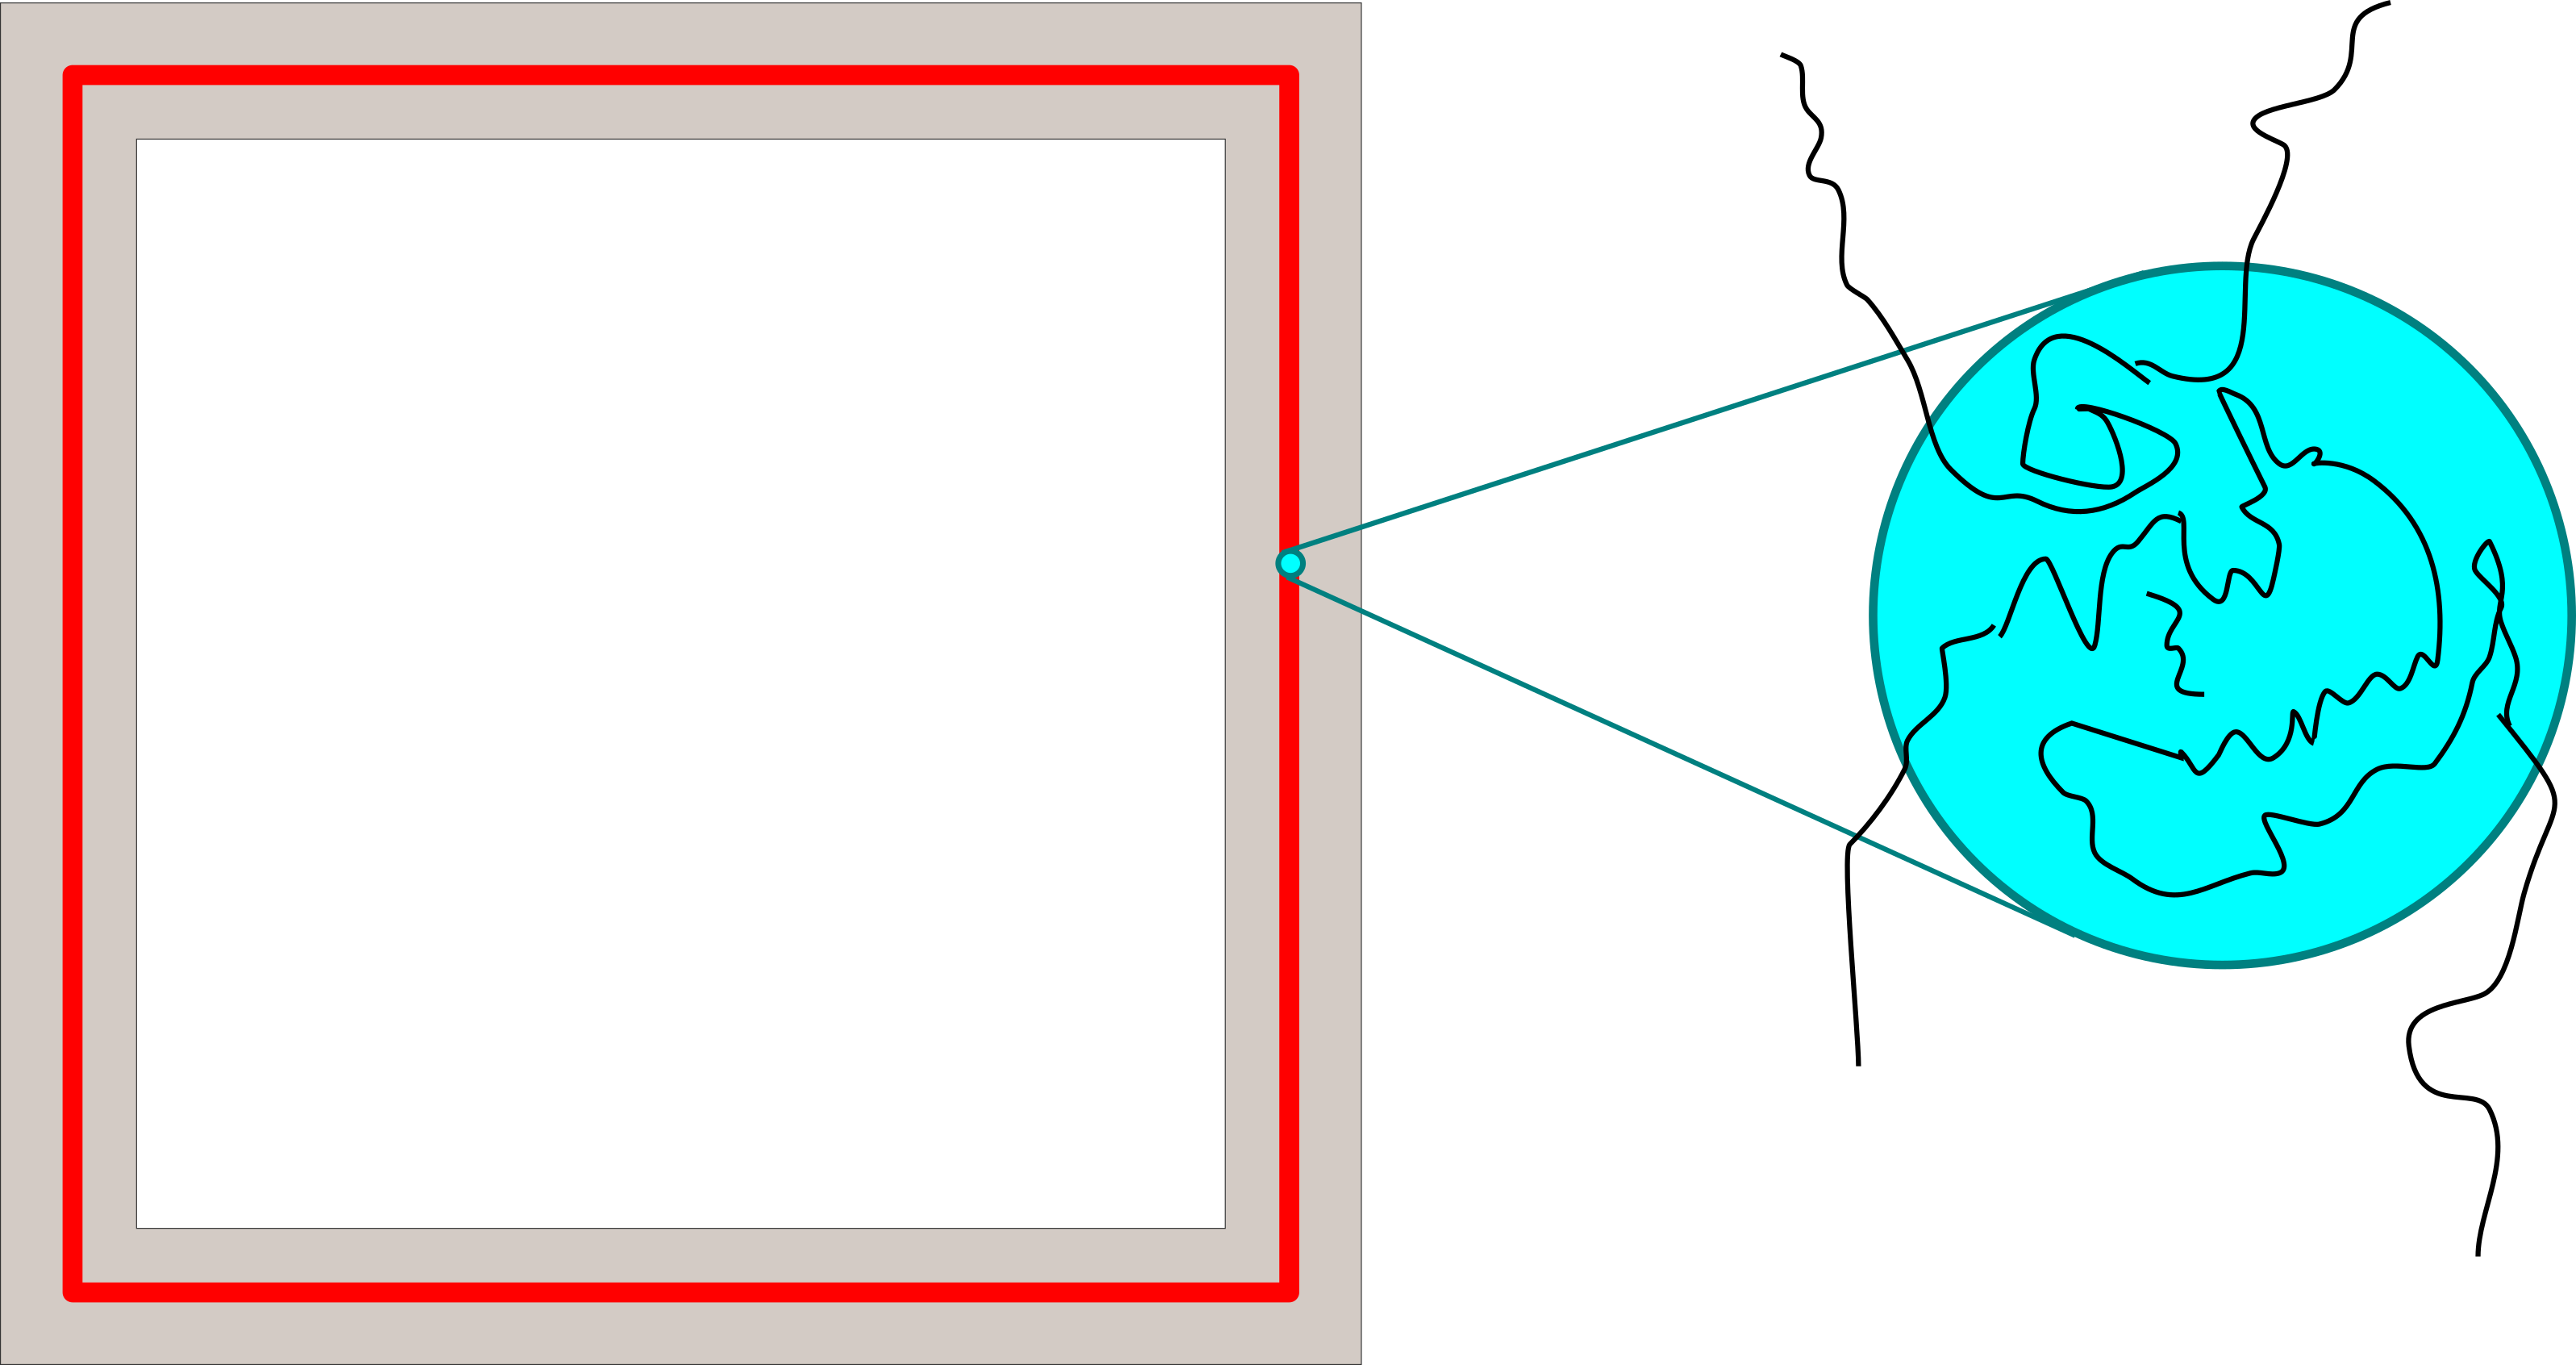
\includegraphics[width=420, alt="A square ring of boundary around an inner square, and a Brownian path that returns to the ring several times"]{barrier-round.png}
\end{columns}
\heading{Other ingredients}
\begin{itemize}
\item pairwise disjoint cubes in \textbf{general position}, \textbf{mixed-scale covers} (next slide), and \textbf{round holes}
\item \textbf{approximate polar integration}: a nearly sharp bound on the potential ${\int|Y-X|^{-(n-2)}\,d\mu(Y)}$ when ${\mu(Q)\leq(\side Q)^s}$ for all cubes $Q$
\end{itemize}
\begin{center}
\textcolor{c4}{The gains are cumulative: five decimals in $\RR^3$ needs all of them together} \goto{app-thm61}{Theorem 6.1}
\end{center}

\slide{A hole helps only if it is big enough}
When $s<n$, splitting a cube into smaller cubes \textbf{increases} $\sum_i(\side Q_i)^s$, even though the total volume stays the same. A hole must be big enough to pay for the split, and covers by cubes of mixed sizes make a hole pay much sooner
\begin{js}[size=1700x520, frames=1, alt="Interactive: a unit square with a hole of side 1/7 in one corner, covered three ways: by one square, by the 48 grid squares of side 1/7 outside the hole, and by one square of side 6/7 plus 12 squares of side 1/7; a slider sets s between 1.95 and 2, and each cover's sum of side lengths to the power s is shown"]
const font = (k, b) => (b ? '600 ' : '') + k + "px 'JetBrains Mono', monospace";
const S = 270, Y0 = 10, XS = [110, 715, 1320], SX0 = 300, SX1 = 1500, SY = 440, LO = 1.95, HI = 2;
canvas.style.touchAction = 'none';
if (state.s === undefined) state.s = 1.98;
const uni = (s) => 48 * Math.pow(7, -s), mix = (s) => Math.pow(6 / 7, s) + 12 * Math.pow(7, -s);
function root(f) { let a = 1.5, b = 2; for (let i = 0; i < 80; i++) { const m = (a + b) / 2; if (f(m) > 1) a = m; else b = m; } return b; }
const tU = root(uni), tM = root(mix);
const trunc = (v, d) => (Math.floor(v * Math.pow(10, d)) / Math.pow(10, d)).toFixed(d) + '…';
const SXof = (s) => SX0 + (s - LO) / (HI - LO) * (SX1 - SX0);
function hole(x0) {
  const c = S / 7, hx = x0 + 6 * c, hy = Y0;
  ctx.fillStyle = '#ffffff'; ctx.fillRect(hx, hy, c, c);
  ctx.strokeStyle = colors.alert; ctx.lineWidth = 3; ctx.setLineDash([7, 6]); ctx.strokeRect(hx, hy, c, c); ctx.setLineDash([]);
}
function frame(x0) { ctx.strokeStyle = colors.ink; ctx.lineWidth = 3; ctx.strokeRect(x0, Y0, S, S); }
function draw() {
  ctx.clearRect(0, 0, w, h);
  const c = S / 7, s = state.s;
  // the set to cover: everything in the square except the hole
  for (const x0 of XS) { ctx.fillStyle = '#E4E7EA'; ctx.fillRect(x0, Y0, S, S); }
  // cover 1: one square
  ctx.fillStyle = 'rgba(30,42,56,0.10)'; ctx.fillRect(XS[0], Y0, S, S);
  // cover 2: the 48 grid squares outside the hole
  ctx.strokeStyle = colors.c1; ctx.lineWidth = 2;
  for (let i = 0; i < 7; i++) for (let j = 0; j < 7; j++) if (!(i === 6 && j === 0)) { ctx.fillStyle = 'rgba(52,96,196,0.16)'; ctx.fillRect(XS[1] + i * c + 2, Y0 + j * c + 2, c - 4, c - 4); ctx.strokeRect(XS[1] + i * c + 2, Y0 + j * c + 2, c - 4, c - 4); }
  // cover 3: one square of side 6/7 and 12 squares of side 1/7
  ctx.strokeStyle = colors.c2; ctx.fillStyle = 'rgba(196,96,20,0.16)';
  ctx.fillRect(XS[2] + 2, Y0 + c + 2, 6 * c - 4, 6 * c - 4); ctx.strokeRect(XS[2] + 2, Y0 + c + 2, 6 * c - 4, 6 * c - 4);
  for (let k = 0; k < 13; k++) { const [i, j] = k < 6 ? [k, 0] : [6, k - 6]; if (i === 6 && j === 0) continue; ctx.fillRect(XS[2] + i * c + 2, Y0 + j * c + 2, c - 4, c - 4); ctx.strokeRect(XS[2] + i * c + 2, Y0 + j * c + 2, c - 4, c - 4); }
  for (const x0 of XS) { hole(x0); frame(x0); }
  ctx.fillStyle = colors.alert; ctx.font = font(26, true); ctx.textAlign = 'left'; ctx.fillText('hole', XS[0] + S + 12, Y0 + 30);
  // the sums
  const rows = [[XS[0], 'one square', '1^s = 1', 1, colors.ink], [XS[1], '48 squares of side 1/7', '48·(1/7)^s', uni(s), colors.c1], [XS[2], '1 + 12 squares', '(6/7)^s + 12·(1/7)^s', mix(s), colors.c2]];
  for (const [x0, lab, f, v, col] of rows) {
    ctx.textAlign = 'center'; ctx.fillStyle = col; ctx.font = font(28, true); ctx.fillText(lab, x0 + S / 2, Y0 + S + 38);
    ctx.font = font(28); ctx.fillStyle = colors.ink; ctx.fillText(f, x0 + S / 2, Y0 + S + 72);
    if (v !== 1) { ctx.font = font(32, true); ctx.fillStyle = v < 1 ? colors.c4 : colors.alert; ctx.fillText('= ' + trunc(v, 4) + (v < 1 ? '  helps' : '  does not help'), x0 + S / 2, Y0 + S + 110); }
  }
  // slider for s
  ctx.strokeStyle = colors.grid; ctx.lineWidth = 10; ctx.lineCap = 'round'; ctx.beginPath(); ctx.moveTo(SX0, SY); ctx.lineTo(SX1, SY); ctx.stroke();
  for (const [t, col, lab] of [[tM, colors.c2, 'mixed helps: s > ' + trunc(tM, 4)], [tU, colors.c1, 'uniform helps: s > ' + trunc(tU, 4)]]) {
    ctx.strokeStyle = col; ctx.lineWidth = 4; ctx.beginPath(); ctx.moveTo(SXof(t), SY - 24); ctx.lineTo(SXof(t), SY + 24); ctx.stroke();
  }
  ctx.fillStyle = colors.alert; ctx.beginPath(); ctx.arc(SXof(state.s), SY, 17, 0, 2 * Math.PI); ctx.fill();
  ctx.fillStyle = colors.ink; ctx.font = font(30, true); ctx.textAlign = 'right'; ctx.fillText('s = ' + state.s.toFixed(3), SX0 - 40, SY + 10);
  ctx.font = font(24); ctx.textAlign = 'right'; ctx.fillStyle = colors.c2; ctx.fillText('mixed helps: s > ' + trunc(tM, 4), SXof(tM) + 10, SY + 58);
  ctx.textAlign = 'left'; ctx.fillStyle = colors.c1; ctx.fillText('uniform helps: s > ' + trunc(tU, 4), SXof(tU) - 10, SY + 58);
  ctx.fillStyle = colors.muted; ctx.textAlign = 'right'; ctx.fillText('2', SX1 + 40, SY + 8);
}
function pos(e) { const b = canvas.getBoundingClientRect(); return [(e.clientX - b.left) * w / b.width, (e.clientY - b.top) * h / b.height]; }
let drag = false;
function set(x) { state.s = Math.round((LO + Math.min(1, Math.max(0, (x - SX0) / (SX1 - SX0))) * (HI - LO)) * 1000) / 1000; }
canvas.onpointerdown = (e) => { const [x, y] = pos(e); if (Math.abs(y - SY) < 45 && x > SX0 - 30 && x < SX1 + 30) { drag = true; set(x); canvas.setPointerCapture(e.pointerId); e.stopPropagation(); } };
canvas.onpointermove = (e) => { if (drag) set(pos(e)[0]); };
canvas.onpointerup = canvas.onpointercancel = () => { drag = false; };
canvas.onclick = (e) => e.stopPropagation();
onFrame(draw);
\end{js}
\begin{columns}[1 1]
\textcolor{c1}{\textbf{Uniform cover:}} a hole helps only if ${n-s\lesssim(\text{volume of the hole})/\log m}$
\columnbreak
\textcolor{c2}{\textbf{Mixed cover:}} a hole helps as soon as ${n-s\leq(\text{volume of the hole})/(n+1)}$
\end{columns}

\slide{An elementary open problem}
What is the $s$-dimensional (cubical) Hausdorff content $\textcolor{c1}{\Haus^s_\infty(B(0,1))}$ of the unit ball?
\begin{columns}[4 4 5]
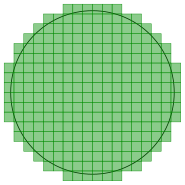
\includegraphics[height=300, alt="The unit disk covered by 256 squares of side 0.12"]{fig-15-175-1.svg}
\textcolor{c1}{256 squares of side $0.12$}: $\;\Haus^{1.75}_\infty(B)\leq6.2633\ldots$
\columnbreak
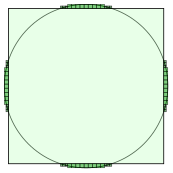
\includegraphics[height=300, alt="The unit disk covered by one square of side 1.9 and small squares near the four arcs left outside it"]{fig-15-175-2.svg}
\textcolor{c2}{1 square of side $1.9$, plus 60 squares of sides $0.05$ and $0.03$}: $\;\Haus^{1.75}_\infty(B)\leq\alert{3.3170\ldots}$
\columnbreak
One square of side $2$: $\;\Haus^{1.75}_\infty(B)\leq2^{1.75}=3.3635\ldots$
\medskip
Optimizing uniform grids:
$$\Haus^s_\infty(B)\leq\omega_n\frac{n^n}{s^s}\left(\frac{\sqrt n}{n-s}\right)^{n-s}$$
\end{columns}
\begin{openproblem}{}
Compute $\Haus^s_\infty(B(0,1))$ exactly for any $n-1<s<n$. To our knowledge, the exact value is unknown even in the plane
\end{openproblem}

% ======================================================================
\section*{How we got there}
\slide{How we got to five decimals}
\begin{js}[size=1680x430, frames=1, alt="Timeline of the number of decimals in the proved bound on d_3: 15 (Badger–Genschaw), then 12 in March 2025, 10 in August, 9 in October, 8 in November, 6 in December 2025, approximate polar integration in spring 2026, and 5 in late August 2026, after AI tools came into use in May 2026"]
const font = (k, b) => (b ? '600 ' : '') + k + "px 'JetBrains Mono', monospace";
const x0 = -4, x1 = 19.4, L = 40, R = 40;
const X = (m) => L + (m - x0) / (x1 - x0) * (w - L - R);
const yA = 230;
ctx.fillStyle = '#E3F2E1'; ctx.fillRect(X(14), 20, X(19.2) - X(14), 340);
ctx.fillStyle = colors.c4; ctx.font = font(28, true); ctx.textAlign = 'center';
ctx.fillText('using AI tools', X(16.6), 58);
ctx.fillStyle = 'rgba(42,85,184,0.25)'; ctx.fillRect(X(12), yA - 9, X(14) - X(12), 18);
ctx.fillStyle = colors.c1; ctx.font = font(24); ctx.fillText('approximate polar', X(12.2), yA - 70); ctx.fillText('integration', X(12.2), yA - 42);
ctx.strokeStyle = colors.axis; ctx.lineWidth = 4;
ctx.beginPath(); ctx.moveTo(X(-1.6), yA); ctx.lineTo(X(19.3), yA); ctx.stroke();
ctx.setLineDash([6, 8]); ctx.beginPath(); ctx.moveTo(X(-2.6), yA); ctx.lineTo(X(-1.6), yA); ctx.stroke(); ctx.setLineDash([]);
function pt(m, d, label, color, r) {
  ctx.fillStyle = color; ctx.beginPath(); ctx.arc(X(m), yA, r || 12, 0, 2 * Math.PI); ctx.fill();
  ctx.font = font(52, true); ctx.textAlign = 'center'; ctx.fillText(d, X(m), yA - 36);
  ctx.fillStyle = colors.ink; ctx.font = font(26); ctx.fillText(label, X(m), yA + 50);
}
pt(-3, '15', 'B–G', colors.muted);
[[0, '12', 'Mar'], [5, '10', 'Aug'], [7, '9', 'Oct'], [8, '8', 'Nov'], [9, '6', 'Dec']].forEach(p => pt(p[0], p[1], p[2], colors.c3));
ctx.strokeStyle = colors.ink; ctx.lineWidth = 3; ctx.beginPath(); ctx.moveTo(X(14), yA - 14); ctx.lineTo(X(14), yA + 14); ctx.stroke();
ctx.fillStyle = colors.ink; ctx.font = font(26); ctx.fillText('May', X(14), yA + 50);
pt(17.5, '5', 'late Aug', colors.alert, 14);
ctx.strokeStyle = colors.muted; ctx.lineWidth = 2;
ctx.beginPath(); ctx.moveTo(X(-0.4), yA + 80); ctx.lineTo(X(9.4), yA + 80); ctx.moveTo(X(9.8), yA + 80); ctx.lineTo(X(19), yA + 80); ctx.stroke();
ctx.fillStyle = colors.muted; ctx.font = font(28); ctx.fillText('2025', X(4.5), yA + 118); ctx.fillText('2026', X(14.4), yA + 118);
\end{js}
\begin{itemize}
\item Each number counts the decimals in the proved bound $d_3<2.99\cdots9$
\item The principal ideas come from more than two years of research and predate our use of AI tools
\item The steps from 15 down to 6 decimals came before we used AI tools
\item The step from 6 to 5 decimals, and the exponent $2n+O(\sqrt n)$ for all $n$, came after
\end{itemize}

\slide{How we used AI}
\textbf{Tools:} Claude Opus 5, Claude Fable 5.1, and GPT 5.6 Sol
\begin{columns}[1 1]
\heading{What they did}
\begin{itemize}
\item symbolic and numerical computation
\item scripts for searches over the discrete parameters of the method, e.g. the ring scale $M$ and the collar scale $L$
\item high-precision and interval-arithmetic checks of the numerical certificates
\item quick tests of variants of the method, most of which we rejected (asymmetric rings, multiple holes)
\item figures and manuscript preparation
\end{itemize}
\columnbreak
\heading{What did not change}
\begin{itemize}
\item \textbf{Everything is proved unconditionally} and verified by the authors
\item Each numerical bound comes from explicit parameters substituted into proved inequalities, and a calculator can check it
\end{itemize}
\begin{note}{}
We could have reached these results eventually, but AI tools compressed months of computation and writing into weeks
\end{note}
\end{columns}

% ======================================================================
\section*{Challenges}

\slide[label=tenchallenges, maxscale=1.3]{Ten challenges}
In the paper, we propose ten intermediate challenges to spur further research. Here $b_n=n-d_n$ is \textbf{Bourgain's constant} \goto{app-challenges1}{statements}
\begin{columns}[1 1]
\begin{enumerate}
\item \textbf{Numerical Experiment} in $\RR^3$
\item \textbf{Explicit Upper Bound}: prove $b_3\leq w<1$ for an explicit $w$
\item \textbf{One Decimal}: prove $b_3\geq0.1$ or $b_3\leq0.9$
\item \textbf{Exact Dimension} in $\RR^3$
\item \textbf{Growing Excess}: dimension excess that grows with $n$
\end{enumerate}
\columnbreak
\begin{enumerate}
\item[6.] \textbf{Exponential Bound}: prove $b_n\geq10^{-Cn}$
\item[7.] \textbf{Packing Dimension} drop. \textcolor{c4}{\textbf{Solved:}} none, by \accent{Guillén-Mola}
\item[8.] \textbf{Maximal Dimension Drop}
\item[9.] \textbf{Denjoy Transition} for Cantor sets in a line. \textcolor{c4}{\textbf{Solved}} by \accent{Cai–Jeznach–Tolsa}
\item[10.] \textbf{Elliptic Bourgain} theorem
\end{enumerate}
\end{columns}

\slide{One Decimal Challenge}
\textbf{Bishop's conjecture:} the Hausdorff dimension of harmonic measure in $\RR^3$ is $2.5$
\medskip
\textbf{Current bounds:} $\;2.005\stackrel{?}{\leq}d_3<\alert{2.99999}$
\begin{challenge}{3, One Decimal}
For trivial reasons, $d_3\leq2.9$ or $d_3\geq2.1$, but we don't know the truth of either bound. Prove one of these (or both)!
\end{challenge}
\begin{itemize}
\item In our view, a resolution of Challenge 3 would be an accomplishment on par with determining the value of $d_3$
\item Even an explicit lower bound is open: find a domain in $\RR^3$ with dimension of harmonic measure $>2+\varepsilon$ for some explicit $\varepsilon>0$ (Challenge 2)
\end{itemize}

\slide{Numerical Experiment Challenge}
\begin{columns}[5 6]
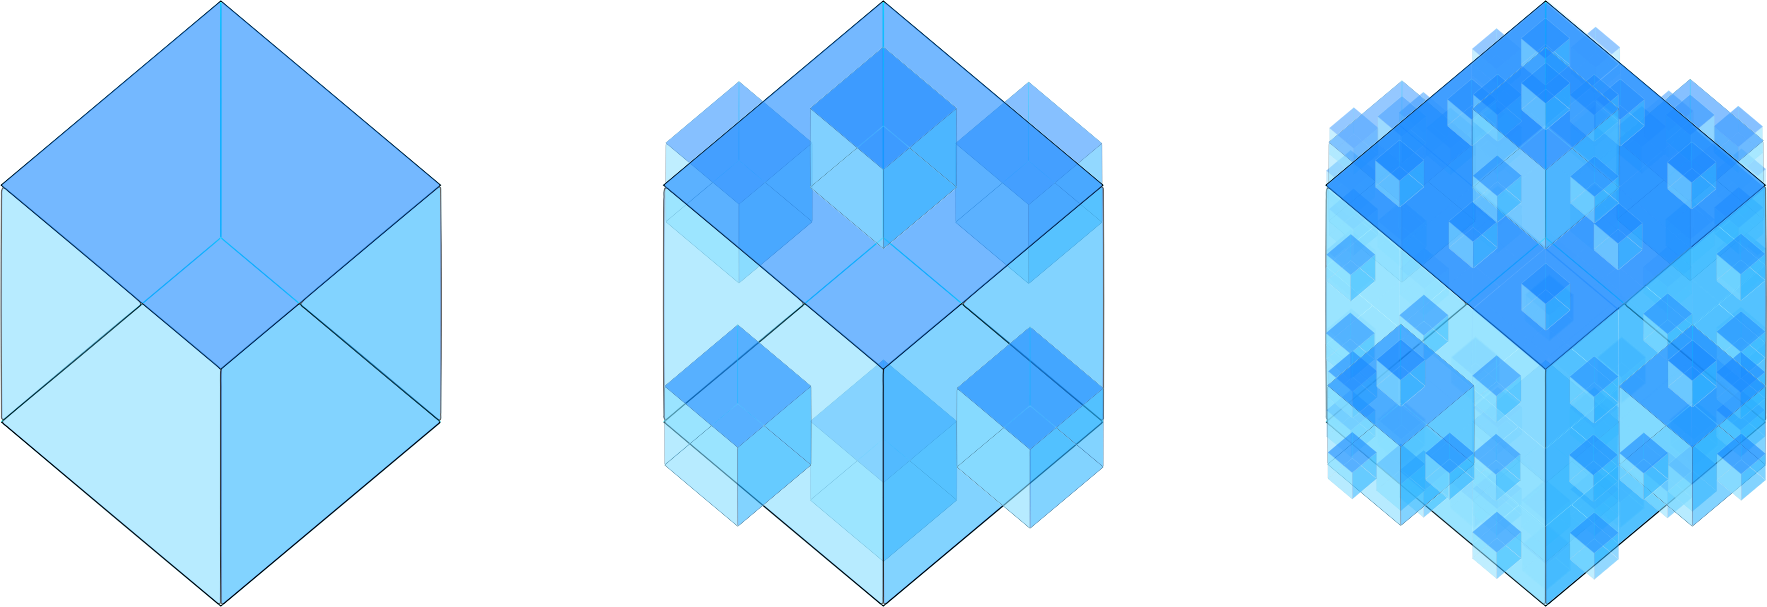
\includegraphics[width=700, alt="Levels 0, 1, 2 of the cubical von Koch snowball"]{physics2.png}
\columnbreak
\begin{itemize}
\item \accent{\textbf{Grebenkov et al. (2005)}} simulated Brownian motion on the fifth stage of the cubical von Koch snowflake $G^3$ and estimated that the dimension of harmonic measure is $\geq2.005$ (not yet mathematically verified)
\item In $\RR^n$, each face of $G^n$ is replaced by $3^{n-1}+2n-2$ faces of relative size $1/3$, so $\textcolor{c3}{\udim\,\omega_{G^n}\leq\log_3(3^{n-1}+2n-2)\to n-1}$. In our view, this is indirect evidence that $\udim\,\omega_{G^3}$ is much smaller than $d_3$
\end{itemize}
\end{columns}
\begin{challenge}{1, Numerical Experiment}
Repeat the experiment to confirm or refute the $2.005$ bound. Estimate the dimension of harmonic measure on other domains in $\RR^3$, e.g. domains whose boundaries are cubical Cantor sets
\end{challenge}

\slide{Exponential Bound Challenge}
\textbf{Bishop's conjecture:} the Hausdorff dimension of harmonic measure in $\RR^n$ is $n-\frac{1}{n-1}$
\medskip
\textbf{Current upper bound:} $\;d_n<n-\left(\frac{1}{n-1}\right)^{2n+6.12\sqrt n}$ for all $n\geq3$
\begin{proposition}{}
No choice of parameters in our model of Bourgain's alternative gives a better lower bound on $n-d_n$ than $\left(\frac{1}{n-1}\right)^{2n}$, up to lower order terms in the exponent
\end{proposition}
\begin{challenge}{6, Exponential Bound}
Prove that $d_n\leq n-10^{-Cn}$ for all $n\geq n_0$ for some constants $C$ and $n_0$, or prove \emph{any} sub-exponential lower bound on $n-d_n$ when $n$ is large
\end{challenge}
\begin{center}
Challenge 6 likely needs a new idea beyond Bourgain's alternative
\end{center}

\slide{Relatives of harmonic measure}
\begin{columns}[6 4]
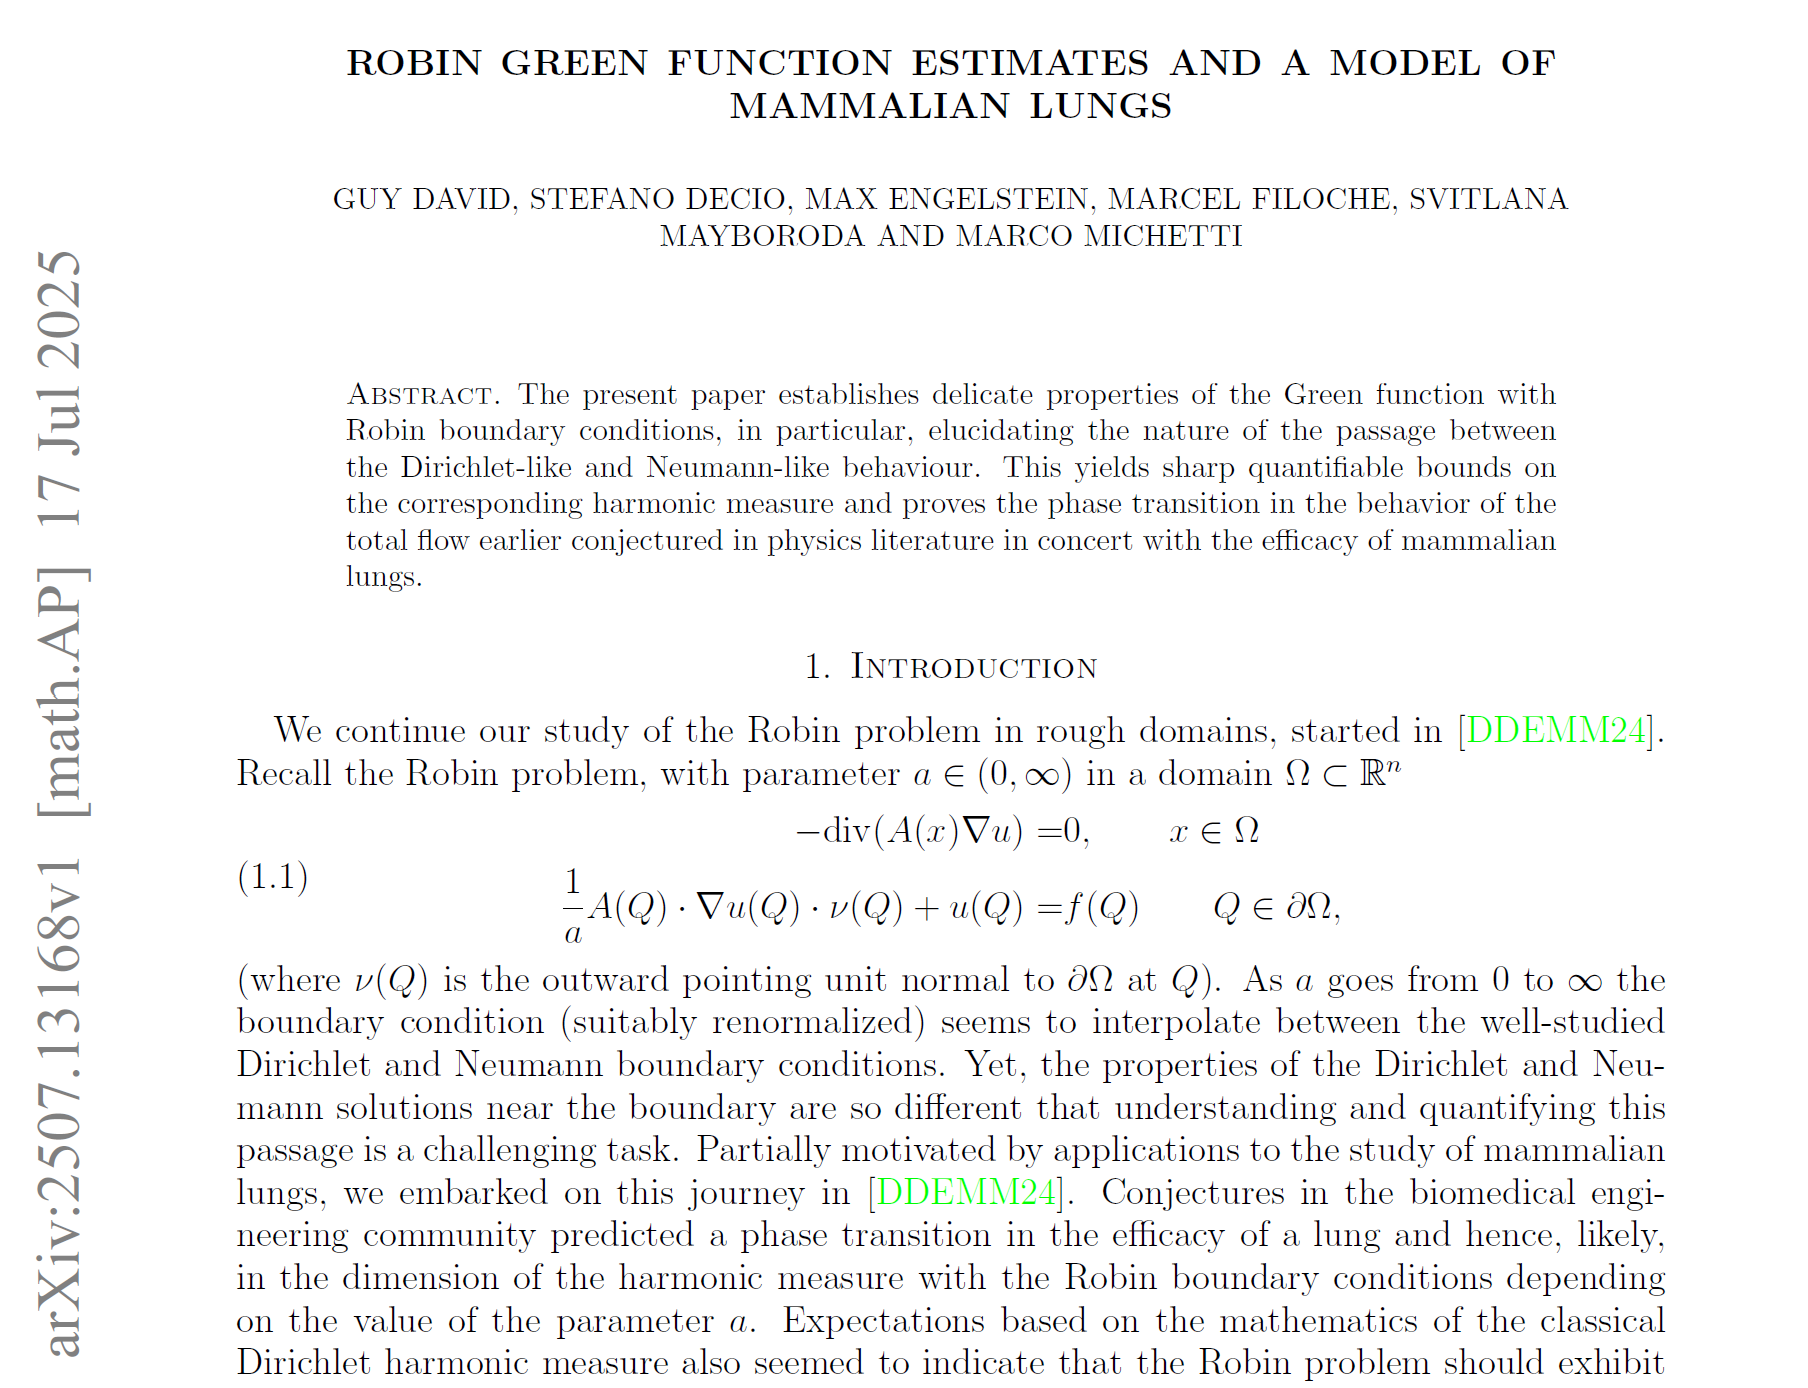
\includegraphics[width=1000, alt="First page of the paper Robin Green function estimates and a model of mammalian lungs by David, Decio, Engelstein, Filoche, Mayboroda, and Michetti"]{mammal.png}
\columnbreak
\begin{center}
\textcolor{c1}{Today I talked about classical harmonic measure, but there are many interesting relatives which are being actively investigated:}
\vspace{1em}
\textcolor{c4}{elliptic measures, $p$-harmonic measures, caloric measure, parabolic measures, harmonic measures in higher co-dimensions, Robin harmonic measures, …}
\end{center}
\end{columns}

\slide[valign=center, align=center]{}
\huge{Thank you for your attention}
\vspace{1.2em}
\large{\textit{One-ring Bourgain alternative and a 5-decimal bound\\ on the dimension of harmonic measure}}

with Michael Albert and Alyssa Genschaw

\href{https://arxiv.org/abs/2610.28037}{arXiv:2610.28037}

% ======================================================================
\appendix
\section*{Appendices}

\slide[label=app-dimlemma, scale=0.8]{Appendix: dimension lemma}
\begin{theorem}{Theorem 4.1}
Let $\mu$ be a Borel regular outer measure on $\RR^n$ that is finite on bounded sets, and let $E\subset\RR^n$ be a Borel set with $\mu(\RR^n\setminus E)=0$. Suppose that there exist $\alpha\in(0,1)$, $\rho\in(0,n)$, $\beta\in(0,1)$, $\tau\in(1,\infty)$, and $\gamma\in(0,1)$ such that every cube $P$ in $\RR^n$ with $\side P\leq1$ satisfies (I) or (II):
\begin{itemize}
\item[\textcolor{c1}{(I)}] there is a cover of $E\cap P$ by pairwise disjoint cubes $Q_1,Q_2,\dots$ contained in $P$ with $\side Q_i\leq\beta\side P$ such that $\textcolor{c1}{\sum_i(\side Q_i)^{n-\rho}\leq(\side P)^{n-\rho}}$
\item[\textcolor{c3}{(II)}] there is a cover of $E\cap P$ by pairwise disjoint cubes $R_1,R_2,\dots$ contained in $P$ with $\side R_i\leq\beta\side P$ such that
$$\textcolor{c1}{\sum_i(\side R_i)^{n-\rho}\leq\tau(\side P)^{n-\rho}}\quad\text{and}\quad\textcolor{c3}{\sum_i\mu(R_i)^\alpha}\textcolor{c2}{(\vol R_i)^{1-\alpha}}\leq\gamma\,\textcolor{c3}{\mu(P)^\alpha}\textcolor{c2}{(\vol P)^{1-\alpha}}$$
\end{itemize}
Then the upper Hausdorff dimension of $\mu$ is at most
$$\alert{n-\frac{\lambda_\alpha}{1+\lambda_\alpha}\,\rho},\quad\text{where }\lambda_\alpha=\frac{-\log_\tau\gamma}{1-\alpha}\in(0,\infty)$$
\end{theorem}

\slide[label=app-thm61, scale=0.8]{Appendix: the one-ring alternative (Theorem 6.1)}
Let $\omega_n$ denote the volume of the unit ball in $\RR^n$. Let $\rho_0=0.2/(n^6\log h)$ and $\eta=\frac{2a}{n+n^{-5}}(1-2^{-(n-2)})$
\begin{theorem}{}
Let $n\geq3$ and $0<a<1$. Let $M\geq3$, $L\geq2$, and $h\geq n^3$ be integers with $2L\geq3M$ such that
$$W=\left(1+\frac{n\,\omega_n}{\omega_{n-1}}\left(\frac{4L}{3M}-1\right)\eta\right)^{-1}<\left(1-\frac{2}{M}\right)^n=V$$
and let $\rho\in(0,\rho_0]$ satisfy
$$\begin{aligned}&\left(1-\tfrac{1}{L}\right)^{n-\rho}+\left(L^n-(L-1)^n-2^{n-1}\right)\left(\tfrac{1}{L}\right)^{n-\rho}+2^{n-1}(2^n-1)\left(\tfrac{1}{2L}\right)^{n-\rho}\\&\quad+\left(2^{n-1}h^n-\tfrac{\omega_n}{2^n}\left(h-2\sqrt n\right)^n\right)\left(\tfrac{1}{2Lh}\right)^{n-\rho}+a\,\omega_n\left(\tfrac{1}{4L}\right)^{n-\rho}\leq1\end{aligned}$$
Then $d_n\leq n-\lambda\rho/(1+\lambda)$, where
$$\lambda=W\log_\tau\frac{W}{V}+(1-W)\log_\tau\frac{1-W}{1-V}$$
$$\tau=\left(1-\frac{2}{M}\right)^{n-\rho}+\big(M^n-(M-2)^n\big)\left(\frac{1}{M}\right)^{n-\rho}$$
\end{theorem}
The five terms count the big cube, the medium cubes, the little cubes, the tiny cubes near the hole, and the hole

\slide[label=app-altI]{Appendix: the partition used in Alternative I}
\begin{columns}[1 1]
\begin{center}
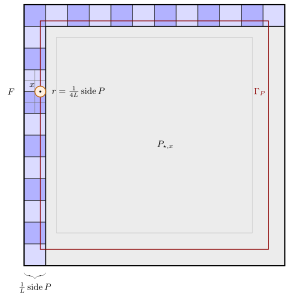
\includegraphics[height=640, alt="The square P with a big cube in one corner and an L-shaped collar of medium squares along two sides"]{fig-x-partition-1.svg}
\end{center}
\columnbreak
\begin{center}
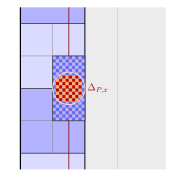
\includegraphics[height=640, alt="Zoom: medium squares near the ball are split into little squares, and little squares near the ball into tiny squares"]{fig-x-partition-2.svg}
\end{center}
\end{columns}
The L-shaped collar is divided into medium cubes. Only those near the ball $B_{P,x}$ are subdivided into little cubes, and only the little cubes covering $B_{P,x}$ are refined into tiny cubes

\slide[label=app-params, scale=0.8]{Appendix: parameters for the lower bounds on $b_n$}
\begin{columns}[5 6]
\heading{Certificates (Theorem 7.2, proved)}
$$\def\arraystretch{1.3}\begin{array}{c|cccc|l}n&M&L&a&h&b_n\geq\\\hline3&9&17&0.585&10^5&1.0118\times10^{-5}\\4&10&17&0.65&10^5&1.206\times10^{-7}\\5&11&19&0.715&10^6&8.006\times10^{-10}\end{array}$$
Plug these into Theorem 6.1 and check the $\rho$-condition with a calculator, at $\rho=1.05628\times10^{-5}$, $1.22747\times10^{-7}$, $8.0084\times10^{-10}$
\columnbreak
\heading{Tuned values (computed, not certified)}
$$\def\arraystretch{1.15}\begin{array}{r|rrrr|ll}n&M&L&a&h&b_n\geq&c_n\\\hline6&13&22&0.750&10^6&3.530\times10^{-12}&2.731\\7&14&25&0.795&10^6&1.166\times10^{-14}&2.558\\8&16&29&0.800&10^6&2.910\times10^{-17}&2.446\\9&18&32&0.855&10^6&5.856\times10^{-20}&2.366\\10&18&37&0.840&10^6&9.128\times10^{-23}&2.310\\50&109&264&0.970&50^6&3.521\times10^{-166}&1.958\\100&254&654&0.990&100^6&4.429\times10^{-384}&1.921\end{array}$$
Computed at 60–80 significant digits. Each value equals $(n-1)^{-c_nn}$, and $c_n$ decreases toward $2$
\end{columns}
\begin{center}
For comparison, Bishop's conjecture is $b_n=(n-1)^{-1}$
\end{center}

\slide[label=app-challenges1, scale=0.8]{Appendix: remaining challenges (1/2)}
\begin{challenge}{4, Exact Dimension}
Construct a domain $\Omega\subset\RR^3$ such that $\udim\,\omega_\Omega>2$ and compute $\udim\,\omega_\Omega$ exactly
\end{challenge}
Wolff constant: $w_\Omega=\udim\,\omega_\Omega-(n-1)$ and $w_n=\sup_{\Omega\subset\RR^n}w_\Omega=1-b_n$
\begin{challenge}{5, Growing Excess}
Construct a family of domains $\Omega^n\subset\RR^n$, for $n\geq3$, arising from a single geometric construction, such that $0<w_{\Omega^3}<w_{\Omega^4}<w_{\Omega^5}<\cdots$. Trivial increases from products $\Omega\times\RR$ do not count
\end{challenge}
Packing analogue of Bourgain's constant: $p_n=n-\sup_{\Omega\subset\RR^n}\overline{\dim}_P\,\omega_\Omega$. Since packing dimension dominates Hausdorff dimension, $0\leq p_n\leq b_n$
\begin{challenge}{7, Packing Dimension}
Prove or disprove that $p_n>0$ for every $n\geq2$. If $p_n>0$, is $p_n=b_n$? In particular, is $p_2=1$?
\end{challenge}
\textcolor{c4}{\textbf{Solved:}} \accent{\textbf{Guillén-Mola 2026}} constructs, for every $n\geq2$, a domain in $\RR^n$ whose harmonic measure has packing dimension $n$. Hence $p_n=0$ for all $n\geq2$ \small{(arXiv:2611.16945)}

\slide[label=app-challenges2, scale=0.8]{Appendix: remaining challenges (2/2)}
Maximal dimension drop constant: $m_n=\sup_{\Omega\subset\RR^n}\left(\dim_H\partial\Omega-\udim\,\omega_\Omega\right)\geq b_n$
\begin{challenge}{8, Maximal Dimension Drop}
For each $n\geq2$, is $m_n=b_n$ or is $m_n>b_n$? If $m_2>1$, compute $m_2$ or obtain nontrivial bounds for it
\end{challenge}
\begin{challenge}{9, Denjoy Transition}
Determine the least $s_0\in(0,1)$ such that, for every $s\in(s_0,1)$ and every $s$-Ahlfors regular compact set $E\subset\RR$, the harmonic measure of $\RR^2\setminus E$ satisfies $\udim\,\omega_{\RR^2\setminus E}<s$. Is there an analogous transition for $s$-Ahlfors regular compact sets $E\subset\RR^2$ not confined to a line?
\end{challenge}
\textcolor{c4}{\textbf{Solved:}} \accent{\textbf{Cai–Jeznach–Tolsa 2026}} show $s_0=1/2$, and find no transition below 1 off the line \small{(arXiv:2610.15805, arXiv:2610.15759)}
\medskip
Elliptic Bourgain constant: $b_n(\Lambda)=n-\sup_{\Omega,A}\udim\,\omega^A_\Omega$ over domains $\Omega$ and $\Lambda$-elliptic symmetric coefficients $A$, so $b_n(1)=b_n$
\begin{challenge}{10, Elliptic Bourgain}
Prove that $b_n(\Lambda)>0$ for every $n\geq3$ and every $1\leq\Lambda<\infty$, and determine the rate at which $b_n(\Lambda)\to0$ as $\Lambda\to\infty$ for each $n\geq2$
\end{challenge}
